\documentclass[14pt]{extbook}
\usepackage[utf8]{inputenc}
\usepackage[T1]{fontenc}
\usepackage[italian]{babel}
\usepackage{lmodern}
\usepackage{lipsum}
\usepackage{multicol}       % Per gestire le colonne
\usepackage{url}
\usepackage{indentfirst}
\usepackage{tipa}
\usepackage{amsmath}
\usepackage{amssymb}
\usepackage{amsthm}
\usepackage{makeidx}
\usepackage{graphicx}
\usepackage{forest}
\usepackage[a-1b]{pdfx}
\usepackage{adjustbox}
\usepackage{longtable}
\usepackage{array}
\usepackage[backend=biber, style=numeric]{biblatex} % Usa Biber come backend
\addbibresource{tesi.bib} % Nome corretto del file .bib
\usepackage{listings}

\usepackage{xcolor} % Per usare colori
\usepackage{hyperref}

\hypersetup{
    colorlinks = true,  % Abilita i link colorati (anziché i box intorno)
    linkcolor = black,   % Colore dei link interni (es. sommario)
    citecolor = black,   % Colore delle citazioni (es. \cite)
    urlcolor = blue,    % Colore degli URL
    filecolor = blue,   % Colore dei link ai file
}

\lstset{
    language=C,
    basicstyle=\ttfamily\footnotesize,
    numbers=left,
    numberstyle=\tiny\color{gray},
    stepnumber=1,
    numbersep=5pt,
    backgroundcolor=\color{lightgray!10},
    showspaces=false,
    showstringspaces=false,
    showtabs=false,
    frame=lines,
    tabsize=4,
    captionpos=b,
    breaklines=true,
    inputencoding=utf8,
    breakatwhitespace=false,
    escapeinside={\%*}{*)},
    literate={ñ}{{\~n}}1
             {ʎ}{{\textturny}}1
             {ʃ}{{\textesh}}1
}



\date{} 


\begin{document}

% Dedica personalizzata
\clearpage
\thispagestyle{empty}
\vspace*{5cm}
\begin{flushright}
    \textit{A chi ha sempre creduto in me.}
\end{flushright}
\clearpage

\begin{center}
    
\includegraphics[width=8cm]{Images/unito-logo.png} \\
    \vspace{0.1cm}
    {\LARGE \textbf{Università degli Studi di Torino}} \\
    \vspace{0.2cm}
    {\Large {Corso di Laurea in Informatica}} \\ 
    \vspace{1cm}
    
    
    {\LARGE \textbf{Gamified Learning per la Dislessia: Lo Sviluppo dell'App "OpenDSA: Reading"}} \\ 
    \vspace{1cm}
    {\Large {Tesi di Laurea}} \\
    \vspace{1cm}
    
\end{center}
    
\begin{multicols}{2}
    \noindent \large{\textbf {Relatore:}} \\
    \large{\textbf{Roberto Esposito}} \\
    \vspace{0.1cm}

    \noindent{\large{\textbf {Candidato:}}} \\
    \large{\textbf{Lorenzo De Marco}} \\
    \large {Matricola 920033}
\end{multicols}
\vspace{0.3cm}
    
\begin{center}
    \large{Anno Accademico 2024/2025}
\end{center}
\newpage

\frontmatter
\tableofcontents
\mainmatter
\pagestyle{plain}


\chapter{Introduzione}
\section{La dislessia}
\subsection{Definizione e criteri diagnostici}
La dislessia, termine che deriva dal greco "dys" (indicante una condizione di inadeguatezza) e "lexis" (riferito al linguaggio), rappresenta una condizione neurologica specifica che influenza l'apprendimento della lettura. Indica una difficoltà specifica nell’acquisizione delle abilità di lettura (correttezza e rapidità) che non è attribuibile a un deficit cognitivo generale, a deficit sensoriali o a condizioni di svantaggio socio-culturale.\\

Secondo il DSM-5 \cite{apa2013dsm}, la dislessia rientra sotto la categoria dei "Disturbi Specifici dell'Apprendimento" con compromissione della lettura. Gli studi di \cite{stella2011dislessia} e come evidenziato da \cite{cornoldi2016reading} hanno contribuito significativamente alla comprensione di questo disturbo nel contesto italiano. Vengono individuati criteri clinici specifici, quali:\\\\

\noindent- Persistenti difficoltà nella lettura di parole singole;\\
- accuratezza e/o velocità nella lettura sostanzialmente al di sotto di quanto atteso per l’età cronologica;\\
- esordio delle difficoltà in età scolare;\\
- significativo impatto sul rendimento scolastico o sulle attività quotidiane che richiedono la lettura.\\

\cite{apa2013dsm}, \cite{ida2024understanding}

\subsection{Prevalenza ed epidemiologia}
Un aspetto importante evidenziato da \cite{eide2011advantage} è che molte persone con dislessia sviluppano capacità cognitive uniche, come una spiccata creatività visuo-spaziale e un'ottima capacità di problem solving, che possono rappresentare vantaggi significativi in determinati contesti professionali e creativi. Le stime di prevalenza della dislessia variano a seconda delle definizioni adottate e dei criteri diagnostici. In generale, si stima che la dislessia interessi dal 3\% al 10\% della popolazione scolastica (stima ipotetica). In Italia, secondo i dati più recenti del MIUR \cite{miur2024dsa}, si è registrato un incremento significativo delle diagnosi, grazie all'implementazione della Legge 170/2010 \cite{legge170_2010} che ha fornito un quadro normativo chiaro per la gestione dei DSA nelle scuole.\\\\

\noindent Possibili motivazioni dell’incremento delle diagnosi:\\

\noindent - Maggior diffusione di conoscenze sulla dislessia;\\
- miglioramento delle procedure di valutazione;\\
- applicazione di normative e linee guida nazionali, come la Legge 170/2010, che tutela gli studenti con DSA.\\
\pagebreak

\subsection{Cause e fattori neurobiologici}

Le basi neurobiologiche della dislessia sono supportate da numerose ricerche in ambito neuroscientifico. Come evidenziato da \cite{cornoldi2016reading} e \cite{shaywitz2003overcoming}, gli studi di neuroimaging hanno mostrato (fMRI, PET, risonanza magnetica strutturale) hanno evidenziato differenze funzionali in alcune aree cerebrali coinvolte nella lettura e nell’elaborazione fonologica, in particolare:\\\\

\noindent\textit{Area temporo-parietale -} essenziale per la corrispondenza suono-simbolo (correlazione tra fonemi e grafemi);\\
\textit{Area occipito-temporale -} deputata al riconoscimento rapido delle parole scritte;\\
\textit{Area frontale inferiore (area di Broca) -} coinvolta nella produzione del linguaggio e nell’elaborazione fonologica.\\

Fattori genetici giocano un ruolo importante: la dislessia ha una tendenza familiare, e diversi geni sono stati associati all’insorgenza del disturbo (ad es. DCDC2, KIAA0319). Ciononostante, è fondamentale sottolineare che i meccanismi genetici non spiegano tutte le variabili e l’ambiente (metodologie didattiche, stimoli culturali) può modulare in parte l’espressione del disturbo.

\subsection{Caratteristiche cliniche e sintomi principali}

Le difficoltà più comuni riguardano:\\

\noindent\textit{Lettura lenta o scorretta:} il bambino o la bambina spesso fa errori di sostituzione, omissione o inversione di lettere.\\
\textit{Difficoltà di decodifica fonologica:} problemi nell’associare i suoni (fonemi) alle lettere scritte (grafemi).\\
\textit{Difficoltà nella comprensione del testo -} la fatica nell’ottenere un’adeguata velocità di lettura influisce sulla comprensione dei contenuti;\\
\textit{Errori ortografici -} sebbene non sempre compaiano nel quadro dislessico puro, possono presentarsi frequenti errori di ortografia legati alla scarsa automatizzazione;\\
\textit{Disfluenza nella lettura ad alta voce -} il bambino può leggere in modo frammentato e monotono;\\

Oltre alle difficoltà di lettura, possono manifestarsi ulteriori problematiche associate, come bassa autostima, scarsa motivazione scolastica e possibili disagi emotivi legati all’esperienza di insuccesso ripetuto.

\subsection{Diagnosi e valutazione}
Un aspetto importante evidenziato da \cite{eide2011advantage} è che molte persone con dislessia sviluppano capacità cognitive uniche, come una spiccata creatività visuo-spaziale e un'ottima capacità di problem solving, che possono rappresentare vantaggi significativi in determinati contesti professionali e creativi. La diagnosi di dislessia viene solitamente effettuata da un team multidisciplinare composto da neuropsichiatri infantili, psicologi e logopedisti. In Italia, i protocolli valutativi prevedono:\\\\

\noindent- Colloquio clinico con i genitori e con il bambino/ragazzo per raccogliere informazioni su sviluppo, storia medica e scolastica.\\
- Test neuropsicologici e prove standardizzate di lettura, per valutare la velocità e l’accuratezza;\\
- Valutazione del quoziente intellettivo (QI) e dello sviluppo cognitivo generale, per escludere disturbi intellettivi;\\
- Screening visivo e uditivo per escludere eventuali deficit sensoriali;\\
- Osservazione del contesto scolastico (quando possibile) per individuare gli ostacoli reali incontrati nell’apprendimento;\\

Un aspetto importante è la diagnosi differenziale rispetto ad altri disturbi dell’apprendimento (disortografia, disgrafia, discalculia) o a possibili comorbilità (es. disturbo da deficit di attenzione/iperattività – ADHD).\\

\subsection{Interventi e strategie di supporto}
Come evidenziato da \cite{masiero2017dsa}, l'intervento sulla dislessia richiede un approccio multidisciplinare che integri aspetti clinici ed educativi, con particolare attenzione al contesto italiano e alle sue specificità. Come suggerito da \cite{stella2011dislessia} e \cite{cornoldi2016linguaggio}, gli interventi più efficaci includono:\\\\

\textbf{Interventi abilitativi e riabilitativi}\\
\noindent \textit{Logopedia:} interventi mirati al potenziamento delle abilità fonologiche e metafonologiche.\\
\textit{Training di lettura:} esercizi graduali che mirano ad automatizzare il processo di lettura. \\
\textit{Software e strumenti compensativi:} sintetizzatori vocali, libri digitali (ebook), mappe concettuali digitali, applicazioni per la gestione dei testi.\\

\textbf{Misure compensative e dispensative a scuola}\\
In Italia, la Legge 170/2010 \cite{legge170} e successivi decreti attuativi hanno introdotto una serie di disposizioni che mirano a garantire il diritto allo studio degli alunni con DSA. Tra queste:\\

\textit{Strumenti compensativi -} utilizzo di audio-libri, calcolatrice, sintesi vocale, mappe concettuali;\\

\textit{Misure dispensative -} riduzione quantitativa dei compiti scritti, valutazione più attenta ai contenuti rispetto alla forma ortografica, tempi più lunghi nelle prove scritte;\\

\textit{Piano Didattico Personalizzato (PDP) -} un documento che definisce gli strumenti e le strategie da adottare in classe e a casa per favorire l’apprendimento;\\

\textbf{Metodologie didattiche inclusive}\\

\noindent\textit{Apprendimento cooperativo -} il lavoro in piccoli gruppi, in cui gli alunni si sostengono a vicenda, favorisce l’inclusione di chi ha difficoltà;\\
\textit{Approcci multisensoriali -} l’uso simultaneo di canali visivi, uditivi e cinestesici (es. Metodo Orton-Gillingham) può migliorare l’associazione tra lettere e suoni;\\
\textit{Mappe e schemi visivi -} organizzano le informazioni in modo chiaro e aiutano la memorizzazione di concetti.\\

\subsection{Aspetti emotivi e psicologici}
La dislessia può avere un impatto significativo sull’autostima e sull’equilibrio emotivo della persona. Spesso, i bambini con dislessia sperimentano ripetuti insuccessi e frustrazioni a scuola, il che può tradursi in:\\\\
	Ansia scolastica o da prestazione;\\
    Demotivazione e rifiuto della lettura;\\
    Sentimenti di inadeguatezza e bassa autostima.\\\\
È fondamentale che genitori e insegnanti sostengano emotivamente il bambino, valorizzandone i progressi e gli interessi, al fine di prevenire l’insorgenza di disturbi emotivi e comportamentali secondari.\\

\subsection{Vita adulta e prospettive future}
La dislessia non scompare con il termine della scuola dell’obbligo; può manifestare i suoi effetti anche nell’età adulta, specialmente in ambito universitario e lavorativo. Tuttavia, molte persone dislessiche sviluppano strategie di compensazione efficaci e, con il giusto supporto, possono raggiungere risultati eccellenti in vari campi professionali.\\\\

\textbf{Università}\\
Le università italiane prevedono spesso servizi di supporto per studenti con DSA (es. uffici di tutorato, servizi di counseling), che offrono strumenti compensativi e misure dispensative per gli esami.\\\\

\textbf{Lavoro}\\
Molti adulti dislessici sviluppano abilità peculiari (ad es. un’elevata creatività, capacità di problem solving, percezione visuo-spaziale) che possono rivelarsi un punto di forza in settori come design, arte, architettura, tecnologia. È importante che l’ambiente di lavoro sia flessibile e includa strategie di organizzazione e comunicazione adeguate.\\\\

\subsection{In breve}
La dislessia è un disturbo complesso, che coinvolge le abilità di lettura e può influire significativamente sulla vita scolastica e professionale della persona. Grazie all’ampia ricerca neurobiologica e psicopedagogica, oggi si comprende molto meglio il disturbo e si dispone di strategie efficaci di diagnosi, intervento e supporto.\\
La sensibilizzazione sociale e la formazione degli insegnanti, unite a un quadro normativo di tutela (come la Legge 170/2010 in Italia), sono fondamentali per creare un contesto educativo inclusivo e rispettoso delle differenze individuali. Una presa in carico globale, che includa aspetti emotivi e relazionali, è essenziale per aiutare chi soffre di dislessia a sviluppare appieno le proprie potenzialità.\\\\
In conclusione, affrontare la dislessia in modo adeguato significa garantire a bambini, ragazzi e adulti l’opportunità di esprimere al massimo le proprie capacità, aiutandoli a gestire le difficoltà e a valorizzare le loro peculiarità. L’approccio integrato e la collaborazione fra scuola, famiglia e specialisti rappresentano la chiave per il successo formativo e personale dei soggetti con dislessia. Ed è questo il motivo fondante che ha portato alla realizzazione di questo Progetto di Tesi che, con un approccio moderno, tenta di individuare un percorso utile a mitigare la condizione di dislessia, al fine di favorire convivenza, accettazione e mitigazione della condizione di dislessia. Tale percorso prevede l’accompagnamento del bambino per un periodo stimato in 200 giorni, durante il quale gli verranno proposti degli esercizi per conoscersi, capirsi e migliorarsi.\\
\pagebreak

\section{L'Avvento delle nuove tecnologie}
\subsection{Il concetto di accessibilità e l’impatto delle tecnologie}
Il concetto di "accessibilità" comprende l'insieme di caratteristiche che consentono a tutte le persone, incluse quelle con disabilità visive, uditive, motorie o cognitive, di utilizzare e beneficiare pienamente di un prodotto, sia esso digitale o fisico. Secondo la classificazione ICF \cite{who2001icf}, l'accessibilità rappresenta un elemento fondamentale per garantire la piena partecipazione delle persone alla vita sociale e professionale. Nel contesto digitale, come definito dal W3C \cite{w3c2024wai}, questo concetto assume particolare rilevanza, specialmente considerando l'evoluzione delle tecnologie assistive e dei framework di sviluppo come quelli utilizzati in OpenDSA: Reading. LL’accessibilità rappresenta, secondo la definizione del W3C \cite{w3c_wai}, un elemento fondamentale nello sviluppo di tecnologie inclusive. Le linee guida WCAG \cite{wcag20} \cite{wcag21} hanno fornito un framework essenziale per lo sviluppo di contenuti digitali accessibili. Possiamo definirla l’insieme di caratteristiche che permettono a tutti gli utenti, compresi coloro con disabilità visive, uditive, motorie o cognitive, di fruire di un prodotto (digitale o fisico) in maniera completa. Prima dell’era digitale, le persone con disabilità incontravano barriere enormi nell’accesso all’informazione, ai servizi e alle opportunità di comunicazione. L’avvento delle nuove tecnologie – in particolare l’evoluzione di internet, dei dispositivi mobili, dei software di riconoscimento vocale e dei lettori di schermo – ha aperto scenari inediti di inclusione.\\\\
Esempi di tecnologie assistive:\\

\textit{Screen reader -} es. JAWS, NVDA, VoiceOver su macOS/iOS, TalkBack su Android per utenti non vedenti o ipovedenti;\\

\textit{Sintesi vocale e ingranditori di caratteri -} per facilitare la lettura dei contenuti;\\

\textit{Tecnologie di puntamento alternative -} trackball, comandi oculari, switch per chi ha difficoltà motorie;\\

\textbf{Software di riconoscimento vocale -} es. Dragon NaturallySpeaking che consentono a utenti con problematiche motorie di interagire col computer tramite la voce;\\

\textit{Dispositivi hardware -} come tastiere Braille, display Braille, sensori e interfacce tattili.\\\\

Grazie alla digitalizzazione e alla crescente standardizzazione, gli sviluppatori possono integrare sin dall’inizio requisiti di accessibilità, facilitando l’uso di prodotti e servizi a una platea sempre più ampia di persone.\\

\subsection{Le WCAG 2.0: linee guida per il web}
Le Web Content Accessibility Guidelines (WCAG) \cite{w3c2008wcag20} \cite{w3c2018wcag21} rappresentano lo standard internazionale per l'accessibilità dei contenuti web. Questi principi hanno guidato anche lo sviluppo dell'interfaccia utente di OpenDSA: Reading, garantendo che l'applicazione sia utilizzabile da utenti con diverse abilità. Uno degli standard più importanti in ambito di accessibilità sul web è rappresentato dalle Web Content Accessibility Guidelines (WCAG). Sviluppate dal World Wide Web Consortium (W3C), in particolare dall’iniziativa WAI (Web Accessibility Initiative), esse offrono un quadro di riferimento completo per rendere i contenuti web utilizzabili da tutti.

\subsection{Origine e struttura delle WCAG}
\textit{WCAG 1.0:} pubblicate nel 1999, furono il primo tentativo di definire un insieme di raccomandazioni per sviluppare siti e applicazioni web accessibili;\\
    
\textit{WCAG 2.0:} pubblicate nel dicembre 2008, hanno introdotto quattro principi fondamentali sintetizzati nell’acronimo POUR (Perceivable, Operable, Understandable, Robust), declinandoli in 12 linee guida e numerosi criteri di successo suddivisi in tre livelli di conformità (A, AA, AAA);\\
    
\textit{WCAG 2.1 (2018) e WCAG 2.2 (in fase di finalizzazione):} versioni aggiornate per tenere conto delle nuove tecnologie (mobile, touch, gesture, etc.) e delle esigenze emergenti.\\

\subsection{I quattro principi fondamentali (POUR)}
\textit{Percepibile (Perceivibile):} le informazioni e i componenti dell’interfaccia devono essere presentati in modo che siano percepibili da tutti i sensi disponibili (vista, udito, tatto), eventualmente tramite alternative (testo alternativo per le immagini, sottotitoli per i video, trascrizioni per i podcast, ecc.);\\

\textit{Utilizzabile (Operable):} la navigazione e l’interazione con gli elementi dell’interfaccia devono essere tali da non costringere a usare un unico strumento di input. Devono prevedere la possibilità di usare tastiera, mouse, touch, comandi vocali, dispositivi speciali, ecc. Inoltre, i contenuti non devono causare reazioni fisiologiche (es. lampeggiamenti troppo veloci possono scatenare crisi epilettiche);\\

\textit{Comprensibile (Understandable):} il contenuto deve essere chiaro, coerente e prevedibile. L’utente deve essere in grado di comprendere come interagire e come ricevere feedback sulle azioni compiute;\\

\textit{Robusto (Robust):} i contenuti e i codici devono essere compatibili con tecnologie assistive e browser diversi, presenti e futuri. Ciò implica l’uso di standard aperti e la separazione tra contenuto e presentazione (HTML semantico, ARIA, CSS adeguato, etc).
\pagebreak

\subsection{Adozione e benefici}
L’adozione delle WCAG 2.0 (e successive) è auspicata da governi e organizzazioni internazionali per:\\

- garantire un principio di uguaglianza e inclusione;\\

- ridurre le barriere tecnologiche e l’esclusione digitale;\\

- migliorare la User Experience (UX) per un’utenza più ampia (anche non disabile, ad esempio utenti anziani o con connessioni lente).\\

\subsection{Sviluppo di software e hardware “user friendly”}
Le tecnologie digitali non si limitano ai siti web. È fondamentale progettare software e hardware inclusivi, secondo un principio di “progettazione universale” (Universal Design), che punti a rendere i dispositivi fruibili dal maggior numero possibile di persone, indipendentemente dalle loro abilità.\\

\subsection{Sviluppo software inclusivo}
    Progettazione centrata sull’utente (UCD)\\
        Coinvolgimento diretto di persone con diverse abilità fin dalle prime fasi di analisi dei requisiti.\\
        Sessioni di “usability testing” con campioni di utenti reali, compresi coloro che utilizzano tecnologie assistive.\\
        Iterazione continua: design → prototipo → test → miglioramenti → ulteriore test.\\

\subsection{Linee guida e toolkit}
Aziende come Microsoft, Apple e Google offrono linee guida specifiche per lo sviluppo di app accessibili (per Windows, macOS/iOS e Android).\\

Framework e librerie front-end (es. Flutter - tecnologia usata all'interno del Progetto di tesi, Angular, React, Vue) includono componenti già ottimizzati per l’accessibilità (ad esempio, con attributi ARIA integrati).\\

\subsection{Rispetto degli standard}
Utilizzo di markup semantico (per il web), di etichette testuali, di controlli navigabili da tastiera, di testo alternativo per immagini, contrasti cromatici adeguati, ecc.\\
        
Inserimento di meccanismi di navigazione chiari (ad es. skip link) per aiutare gli utenti con screen reader o con mobilità ridotta.\\

\subsection{Sviluppo hardware inclusivo}
Design ergonomico: forme, pulsanti e materiali devono ridurre lo sforzo fisico e facilitare la presa, specialmente per chi ha problemi di destrezza manuale o di coordinamento.\\

Interfacce multisensoriali: l’uso di feedback aptici (vibrazioni), indicatori sonori o luminosi permette a persone con deficit uditivi o visivi di interagire con i dispositivi.\\

Compatibilità con dispositivi assistivi: per esempio, predisposizione di porte e protocolli che consentano a dispositivi medici o sistemi di controllo alternativi di integrarsi facilmente.\\

\subsection{Esempi pratici di tecnologie e progetti inclusivi}
Microsoft Inclusive Design: un insieme di principi e toolkit elaborati da Microsoft per progettare software (come Office, Windows) e servizi (come Xbox) che siano utilizzabili da tutti.\\
    
Apple Accessibility: Apple integra da anni funzioni di accessibilità a livello di sistema operativo (VoiceOver, Zoom, Switch Control, Live Captions, ecc.), dimostrando come l’hardware (touchscreen di iPhone e iPad) e il software (iOS, macOS) possano lavorare congiuntamente per facilitare l’uso da parte di persone cieche, ipovedenti o con limitazioni motorie.\\

Google Accessibility: Android e Chrome OS includono TalkBack (screen reader), comandi vocali, funzioni di ingrandimento e un ecosistema di app e servizi compatibili con standard WCAG e ARIA.\\

Le Distribuzioni Linux: integrano da sempre opzioni legate all'accessibilità, grazie soprattutto alla facoltà di poter manipolare tutto l'ambiente visivo a piacimento. Essi di fatti consentono di creare diversi ambienti che integrano automaticamente diverse agevolazioni in termini di Accessibilità, tra cui: VoiceOver, facoltà di manipolare la grandezza del testo e delle icone a piacere, ecc. Di fatti, diversi Progetti software prendono spunto da queste straordinarie potenzialità degli Ambienti Grafici Linux per creare progetti software ad hoc gratuiti per il mondo scuola (So.di.Linux e UfficioZeroLinux OS Educational ne sono un esempio italiano lampante, il primo sviluppato dal CNR, il secondo da SIITE Srls).\\

Progetti open source: NVDA (Non Visual Desktop Access), uno screen reader gratuito per Windows, sviluppato con il contributo di una community internazionale.\\

Ognuno di questi ambienti software offre API e linee guida affinché gli sviluppatori di terze parti possano realizzare app e siti accessibili fin dalla fase di progettazione.

\subsection{Benefici secondari dell’accessibilità}
Un aspetto spesso sottovalutato è che progettare tecnologie accessibili non avvantaggia solo le persone con disabilità, ma migliora l’esperienza d’uso per tutti. Ad esempio, un’interfaccia chiara e semplificata aiuta chiunque a orientarsi più rapidamente; l’approccio “mobile-first”, quindi testi ben dimensionati, contrasti elevati, layout adattivi, migliora l’esperienza dei dispositivi mobili; un contenuto web con testo alternativo, SEO (Search Engine Optimization), titoli semantici e struttura ordinata risulta più facilmente indicizzabile dai motori di ricerca; infine, i contenuti robusti e compatibili con varie modalità di accesso, adattandosi, durano nel tempo e non “invecchiano” rapidamente al cambiare delle tecnologie.

\subsection{Legislazione e normative di riferimento}
In molti Paesi, esistono leggi e normative che impongono o incoraggiano l’adozione di standard di accessibilità. Il quadro normativo europeo \cite{eu2016_2102}, americano \cite{section508_1998} e italiano italiano \cite{legge_stanca_2004} definisce:\\

\textbf{Unione Europea:}\\
- Direttiva (UE) 2016/2102 sull’accessibilità dei siti web e delle applicazioni mobili degli enti pubblici.\\
- European Accessibility Act (2019), che introduce requisiti di accessibilità per una vasta gamma di prodotti e servizi digitali.\\\\

\textbf{Stati Uniti:}\\
- Section 508 del Rehabilitation Act (aggiornato nel 2017 in armonia con le WCAG 2.0 AA).\\
- Americans with Disabilities Act (ADA), che impone l’accessibilità anche nei servizi digitali.\\

\textbf{Italia:}\\
- Legge Stanca (Legge n. 4/2004), integrata da vari decreti attuativi, che prevede l’obbligo di accessibilità dei siti della Pubblica Amministrazione (e, in parte, dei soggetti privati con particolari requisiti di servizio al pubblico).\\

Questa cornice legislativa spinge le organizzazioni a implementare i principi delle WCAG e a progettare prodotti e servizi accessibili.\\

\subsection{Prospettive future}
L’avvento delle nuove tecnologie ha rivoluzionato il modo in cui le persone con diverse abilità possono accedere alle informazioni, interagire con gli altri e partecipare attivamente alla società. Le WCAG 2.0 – e le versioni successive come la 2.1 e la prossima 2.2 – rappresentano uno standard consolidato per rendere i contenuti web più inclusivi, mentre il concetto di universal design indica la direzione da seguire nello sviluppo di software e hardware realmente “user friendly”.\\
La sfida futura è andare oltre la semplice conformità normativa e puntare a un’accessibilità integrata in ogni fase di progettazione. Coinvolgere utenti con disabilità nei processi di sviluppo, adottare metodologie di progettazione partecipata e curare i dettagli dell’esperienza d’uso garantisce prodotti migliori per tutti e genera un impatto positivo sia dal punto di vista sociale che economico.\\
Le tecnologie continueranno a evolvere (intelligenza artificiale, realtà aumentata, robotica, Internet of Things) e sarà essenziale mantenere il focus sull’accessibilità, evitando di creare nuove barriere. Costruendo dispositivi e servizi universali, si garantisce la piena partecipazione di tutti i cittadini, promuovendo inclusione, pari opportunità e innovazione responsabile.\\
In sintesi, la tecnologia rappresenta oggi un potente alleato per le persone con problemi di accessibilità, a patto che sia sviluppata seguendo principi, standard e buone pratiche che tengano conto di tutte le possibili esigenze. L’innovazione, se accompagnata dall’impegno per l’inclusività, può davvero abbattere barriere secolari e garantire a tutti pari diritti e opportunità di partecipazione. Questo credo, è stato il motivo fondante che ci ha fatto decidere di affrontare il problema della dislessia con le nuove tecnologie emergenti.
\pagebreak

\section{L'approccio alla dislessia con le nuove tecnologie}
\subsection{L'informatica ed i moderni approcci tecnologici}
L'Informatica, negli anni, ha sviluppato l'abilità camaleontica di potersi approcciare a diversi campi scientifici in modo efficace, proponendo soluzioni software ed ingegneristiche capaci di innovare e consentire di avere un punto di vista nuovo del problema che si stava affrontando inizialmente (si pensi alle soluzioni finanziarie, mediche, farmaceutiche, ecc).\\

L'Idea del progetto di tesi nasce da questa innata capacità, consentendo di unire nuove tecnologie come l'Intelligenza Artificiale, con l'uso di linguaggi di programmazione moderni e adatti alla creazione di applicazioni nuove.\\

Poiché il progetto ha come focus principale la dislessia, deve concentrarsi sul trovare una soluzione stand-alone, semplice, intuitiva, di facile utilizza e moderna che consentisse all'utente finale di poter usare l'applicazione, per sviluppare una maggiore confidenza con la propria condizione. Si è deciso di optare per l'uso di tecnologie come:\\

\textbf{Software di riconoscimento vocale (Speech-to-text)} – i programmi che trasformano la voce in testo e che aiutano chi ha difficoltà a trascrivere o a scrivere correttamente e in modo fluido – e di personalizzare la fruizione dei contenuti in modo che possano rispondere alle esigenze di ciascuno studente con dislessia. Ad esempio:\\

\textit{Modifiche del font e della spaziatura -} alcuni font (come OpenDyslexic, Dyslexie Font o font ad alta leggibilità) sono studiati per rendere le lettere più distinguibili fra loro e ridurre gli errori di inversione o salto di riga;\\

\textit{Adeguamento del contrasto e dei colori -} tablet, e-reader e smartphone consentono di regolare facilmente lo sfondo e la dimensione del testo, migliorando la percezione visiva.\\

\textit{Riduzione delle distrazioni -} alcune applicazioni o estensioni del browser favoriscono la lettura a schermo intero, bloccando elementi che possano distrarre (banner, pop-up, ecc.).\\

In questo modo, lo studente con dislessia può configurare l’ambiente di studio secondo le proprie preferenze e necessità, minimizzando gli ostacoli legati alla lettura tradizionale.\\

Affidarsi a strumenti digitali non significa “barare” o aggirare il problema, ma potenziare le abilità dell’allievo e renderlo più indipendente. Tra i benefici possibili segnaliamo:\\

\textit{riduzione dell’errore ortografico -} grazie ai correttori automatici, il ragazzo o l’adulto con dislessia può dedicarsi alla stesura di testi concentrandosi sul contenuto, senza essere ostacolato dagli errori ortografici.\\

\textit{semplificazione della fase di studio -} l’uso di audiolibri, ebook e app per la sintesi vocale permette di leggere (o ascoltare) più materiali, con meno fatica.\\

\textit{aumento dell’autostima -} sentirsi in grado di gestire compiti scolastici o lavorativi in autonomia incrementa la fiducia in sé stessi e diminuisce lo stress.\\

\subsection{Prospettive future}
Utilizzare le nuove tecnologie per affrontare la dislessia non significa sostituire l’intervento didattico tradizionale o l’eventuale supporto logopedico/psicologico, ma integrare entrambi con soluzioni innovative. Ciò consente di:\\\\
- Ridurre le barriere all’apprendimento, stimolando l’interesse e la partecipazione;\\\\
sviluppare competenze metacognitive e strategie di studio personalizzate.\\\\
Promuovere un senso di autonomia e autostima, che incide positivamente sul benessere complessivo della persona;\\\\
In definitiva, l’investimento in tecnologie assistive e in un uso consapevole dei dispositivi digitali è uno dei modi più efficaci per supportare chi ha dislessia e massimizzare le potenzialità di ciascuno.\\

\pagebreak
\section{Il ruolo della IA generativa nel campo DSA}
\subsection{Cosa si intende per Intelligenza Artificiale generativa}
Come delineato da \cite{russell2021artificial}, l'Intelligenza Artificiale generativa rappresenta una delle frontiere più promettenti nel campo dell'IA. Le ricerche condotte da organizzazioni come OpenAI \cite{openai2024research} e DeepMind \cite{deepmind2024research} hanno contribuito significativamente all'evoluzione di questa tecnologia, aprendo nuove possibilità anche nel campo del supporto educativo per persone con DSA. L’Intelligenza Artificiale generativa (o Generative AI) è un ramo dell’IA focalizzato sulla creazione di contenuti nuovi, come testi, immagini, suoni o video, partendo da modelli di apprendimento capaci di imitare e “ri-elaborare” i dati a cui sono stati esposti. Diversamente dai sistemi di AI che si limitano a classificare o riconoscere pattern (pattern recognition), la Generative AI genera appunto nuovi contenuti, spesso sorprendenti anche per gli stessi sviluppatori. Il concetto di Intelligenza Artificiale, teorizzato già da Turing \cite{turing1950computing}, ha visto una svolta significativa con l'introduzione dei modelli Transformer \cite{vaswani2017attention}, che hanno rivoluzionato l'elaborazione del linguaggio naturale. \\
\subsection{Le radici storiche dell’IA dagli albori ai pri- mi modelli generativi: un breve rassegna cronologica}
\subsubsection{Gli inizi dell’IA (anni ‘50-‘70)}
Alan Turing (1950), nel suo articolo “Computing Machinery and Intelligence” \cite{turing1950computing}, propose il celebre “Test di Turing”, aprendo la strada alle riflessioni sull’intelligenza delle macchine. Successivamente John McCarthy e Marvin Minsky \cite{mccarthy1955proposal}, considerati tra i fondatori dell’IA come disciplina accademica, coniarono il termine “Intelligenza Artificiale” (1956) durante il Dartmouth Conference. \\
In questa fase, tuttavia, i primi algoritmi di IA erano di tipo sim- bolico e si concentravano su problemi di logica, algebra e puzzle. Non si parlava ancora di “creatività artificiale” o generazione di contenuti.\\

\subsection{L’avvento dei sistemi conversazionali (anni ‘60-‘70)}

ELIZA (Joseph Weizenbaum, 1966): Il sistema ELIZA \cite{weizenbaum1966eliza} rappresentò uno dei primi sistemi conversazionali, concepito per simulare uno psicoterapeuta rogersiano. Non era un modello generativo in senso stretto, ma aprì la porta a programmi in grado di elaborare risposte testuali (pur basandosi su pattern fissi). \\

Questi pionieri dimostrarono che le macchine potevano “produrre” contenuti linguistici, seppur in maniera molto limitata.\\

\subsection{Il salto di qualità: reti neurali e apprendimento profondo}
\subsubsection{La rinascita delle reti neurali (anni ‘80-‘90)}

Reti neurali artificiali: Già dagli anni ‘40 e ‘50 erano state ipotizzate (McCulloch e Pitts), ma solo negli anni ‘80-‘90, grazie a Backpropagation (metodo di addestramento efficiente), ricominciarono a diffondersi.\\

Tuttavia, la potenza computazionale e la disponibilità di dati rimanevano limitate, e il focus principale era sul riconoscimento di pattern piuttosto che sulla generazione di contenuti.\\

\subsection{L’era del Deep Learning (anni 2000-2010)}

Con l’aumento esponenziale della potenza di calcolo (GPU, cluster di server, cloud computing) e dei “big data” disponibili, gli algoritmi di Deep Learning iniziarono a ottenere prestazioni inedite:\\

\textit{Convolutional Neural Networks (CNN) –} eccellenti per la visione artificiale;\\

textit{recurrent Neural Networks (RNN) –} utili per l’elaborazione del linguaggio naturale;\\

È in questa fase che si prepara il terreno per i modelli generativi più avanzati.\\
\subsection{La svolta generativa: dalle GAN ai Transformer}
\subsubsection{Generative Adversarial Networks (GAN)}
Nel 2014 Ian Goodfellow e i suoi colleghi pubblicano l’articolo “Generative Adversarial Nets”, presentando un’architettura rivoluzionaria.\\

L’introduzione delle GAN \cite{goodfellow2014gan} e successivamente dei Transformer \cite{vaswani2017attention}consistono in due reti neurali (un “generatore” e un “discrimina- tore”) che si addestrano l’una contro l’altra, migliorando progressiva- mente la qualità dei contenuti generati (inizialmente, immagini).\\

Questa innovazione ha aperto la porta alla generazione di immagini realistiche, al deepfake e a un’intera gamma di applicazioni creative.\\

\subsection{La rivoluzione dei Transformer}
“Attention Is All You Need” (\cite{vaswani2017})è il paper che ha introdotto l'architettura "Transformer", segnando un punto di svolta nell'elaborazione del linguaggio naturale. I modelli Transformer, a differenza delle RNN, possono processare in parallelo intere frasi o paragrafi, grazie al meccanismo di "attenzione". Questo approccio innovativo ha dato vita ai grandi modelli di linguaggio (Large Language Models, LLM) come BERT (Google), GPT (OpenAI) e successivi. L'architettura Transformer ha reso possibile la Generative AI basata sul linguaggio ad altissimi livelli, permettendo la creazione di testi coerenti e di tipo "umano" che oggi utilizziamo quotidianamente in varie applicazioni e servizi.\\

\subsection{L’impatto culturale della Generative AI}
\subsubsection{Epoca di “creatività aumentata”}
La Generative AI non è più solo uno strumento tecnico, ma un fenomeno culturale che riguarda diversi settodi. Ad esempio:\\

\textit{arte digitale e design -} Strumenti come DALL-E, Midjourney, Stable Diffusion generano immagini artistiche e trasformano il ruolo di designer e artisti, che diventano “curatori” o “co-creatori” con l’IA.\\

\textit{testi e contenuti online -} Modelli come GPT (Generative Pretrained Transformer) sono in grado di scrivere articoli, riassunti, persino codice di programmazione, con un livello di fluidità mai visto prima.\\

\textit{Musica e audio -} Sistemi in grado di comporre brani musicali o di imitare la voce umana con elevatissima fedeltà.\\

\subsection{Rivoluzione sociale ed economica}
L'avvento di strumenti di Intelligenza Artificiale generativa accessibili tramite Internet ha determinato una profonda democratizzazione delle tecnologie avanzate. Piattaforme come ChatGPT hanno abbattuto le tradizionali barriere d'accesso, rendendo capacità computazionali sofisticate disponibili non solo a specialisti del settore, ma a chiunque disponga di una connessione Internet. Questa rivoluzione ha trasformato radicalmente il panorama tecnologico, consentendo a persone con diversi livelli di competenza tecnica di sfruttare il potenziale dell'IA per risolvere problemi, creare contenuti e ampliare le proprie capacità.\\

Il dibattito etico sull'IA generativa è diventato centrale nella discussione pubblica. I deepfake e la creazione di contenuti ingannevoli sollevano serie preoccupazioni su responsabilità, privacy e autenticità nell'era digitale. Queste tecnologie hanno spinto legislatori e società civile a confrontarsi urgentemente sulla necessità di nuovi paradigmi etici che possano bilanciare l'innovazione con la tutela dei diritti fondamentali.\\

Stanno emergendo rapidamente nuove professioni nell'ecosistema dell'IA. Il "prompt engineering" - l'abilità di formulare istruzioni ottimali per i sistemi di intelligenza artificiale - si afferma come competenza chiave, mentre si sviluppano ruoli specializzati per guidare, verificare e perfezionare l'output dei sistemi generativi.\\

\subsection{Perché l'IA è stata (ed è) rivoluzionaria}
L'intelligenza artificiale ha trasformato radicalmente il panorama tecnologico moderno. Ha democratizzato l'accesso alle capacità creative, permettendo a chiunque di generare rapidamente idee e contenuti, e ha ridefinito i confini dell'automazione, affrontando sfide complesse che prima erano esclusivamente umane. Sul piano sociale, la Generative AI ha sollevato importanti questioni etiche su originalità, copyright e veridicità dell'informazione. Inoltre, l'evoluzione dai metodi tradizionali di Machine Learning verso architetture avanzate come Transformer e GAN ha accelerato enormemente la ricerca in questo campo, producendo un impatto paragonabile alle maggiori rivoluzioni tecnologiche del secolo scorso.\\

\subsection{In breve}
Come evidenziato da \cite{russell2021artificial} e \cite{mitchell2019guide}, l'evoluzione dell’Intelligenza Artificiale generativa racchiude diverse fasi: dalle prime intuizioni simboliche degli anni ’50 alle moderne architetture neurali basate sui Transformer. Nel momento in cui i modelli di IA hanno iniziato a generare contenuti (testi, immagini, musica), ci si è trovati di fronte a una svolta che ha inciso profondamente non solo sulla ricerca tecnologica, ma anche sull’immaginario collettivo e sulla cultura di massa.\\

Oggi, la Generative AI rappresenta una nuova forma di creatività “aumentata” e solleva questioni etiche, sociali ed economiche senza precedenti, spingendo l’umanità a interrogarsi sul confine tra l’umano e l’artificiale, tra l’originale e l’elaborato. È, a tutti gli effetti, una rivoluzione tecnologica e culturale destinata a imprimere una traccia indelebile nella storia.\\

Ragion per cui, visto l'incredibile potenziale rivelato, non poteva che essere una valida opzione d'uso nell'automazione di processi complessi come ad esempio il riconoscimento linguistico della lettura di un bambino dislessico. Processo complesso e spesso soggetto ad errore quando demandato ad uno sppech-to-text tradizionale, ma che si è rivelato nel tempo molto efficace con l'ausilio e l'uso dell'intelligenza artificiale generativa, rinforzando l'idea che alla base di questi cambiamenti, i nuovi approcci e le nuove tecnologie, sono sempre più efficaci con il passare dei loro sviluppi nel tempo.\\
\pagebreak
\clearpage

\chapter{Tecnologie utilizzate}
\section{Il Framework Flutter}
Flutter è un \textit{software development kit} (SDK) open source creato da Google\cite{google2017flutter} che permette lo sviluppo di interfacce utente (UI) nativamente compilate per diverse piattaforme, tra cui Android, iOS, web e desktop, il tutto partendo da un unico codice sorgente. Flutter ha dimostrato la sua efficacia non solo nello sviluppo di applicazioni mobile, ma anche nell'ambito dell'accessibilità, seguendo le linee guida definite dalla direttiva europea \cite{eu2016_2102} sull'accessibilità dei contenuti digitali. Sin dal suo debutto, Flutter è stato considerato particolarmente \emph{rivoluzionario} grazie a:
\begin{itemize}
    \item L'utilizzo del linguaggio \textbf{Dart}, sviluppato anch'esso da Google;
    \item un motore grafico ad alte prestazioni, chiamato \emph{Skia}, che consente un rendering veloce e uniforme delle interfacce;
    \item un approccio \emph{reactive}, in cui la UI si aggiorna dinamicamente in risposta ai cambiamenti di stato;
    \item la filosofia ``\emph{write once, run anywhere}'', che riduce i tempi di sviluppo su più piattaforme.
\end{itemize}

\section{Cenni storici}
\subsection{Il progetto Sky: i prodromi di Flutter}
Come documentato in \cite{flutter2018overview}, Flutter si distingue per la sua architettura innovativa che permette di mantenere prestazioni native su tutte le piattaforme. La funzionalità di hot reload \cite{flutter2023reload} ha rivoluzionato il processo di sviluppo, permettendo modifiche in tempo reale all'interfaccia. L'ecosistema di pacchetti \cite{pubdev2023packages} fornisce inoltre una vasta gamma di componenti riutilizzabili, molti dei quali sono stati integrati in OpenDSA: Reading per ottimizzare il processo di sviluppo.
Flutter ha le sue radici in un progetto sperimentale di Google chiamato \textbf{Sky}, presentato per la prima volta nel 2015 durante il Dart Developer Summit. L’intenzione iniziale era di realizzare un motore grafico e un set di librerie in grado di rendere interfacce utente ad altissime prestazioni sul sistema operativo Android, partendo dal linguaggio Dart.

\subsection{L’annuncio ufficiale di Flutter}
È nel 2017, durante il Google I/O, che Flutter viene presentato al pubblico come SDK multipiattaforma (inizialmente in alpha). Sin da subito, Google punta sull’idea di creare un framework UI “reactive” che potesse unificare lo sviluppo su diverse piattaforme (Android, iOS) mantenendo alte prestazioni e un controllo completo sul rendering.\\

\subsection{Versione stabile e adozione in crescita}
La prima versione stabile di Flutter (\texttt{v1.0}) avviene a dicembre 2018. L’evento viene celebrato come una pietra miliare per lo sviluppo mobile: offriva già allora la possibilità di scrivere app “nativamente compilate” in un unico codice sorgente, con un rendering engine personalizzato e reattivo.\\

\section{Perché Flutter è stato rivoluzionario?}
\subsection{Unico framework per più piattaforme}
Il mantra \emph{cross-platform} non era nuovo, ma soluzioni precedenti come PhoneGap o Cordova non garantivano le stesse prestazioni di un'app nativa. L'implementazione del motore di rendering Skia in Flutter ha consentito un significativo miglioramento nell'esperienza utente, garantendo prestazioni native su diverse piattaforme, che disegna la UI in modo indipendente dalla piattaforma sottostante\cite{google2015sky}.\\

A differenza di altri framework cross-platform, Flutter non si affida ai componenti nativi della piattaforma (come le UIViews su iOS o i widget Android), al contrario, gestisce direttamente il rendering di tutti i componenti UI tramite il motore Skia, utilizzato anche da Google Chrome.\\

\textit{Benefici:}\\

- Coerenza dell’aspetto grafico su tutte le piattaforme.\\
- Elevate prestazioni grazie al rendering su GPU.\\
- Controllo totale sul design e sui widget, senza passare da “ponti” nativi.\\

\subsection{Hot Reload e sviluppo rapido}
Un elemento spesso elogiato dagli sviluppatori è la funzione di \emph{Hot Reload}: ogni modifica al codice sorgente viene istantaneamente riflessa sull'interfaccia (senza ricompilare o ricaricare l'app per intero). Questo approccio incrementa la produttività e riduce i tempi di \emph{debug} e sperimentazione.\\

La funzionalità, oltre ad essere molto utile, rappresenta una \emph{Rivoluzione} nel campo dello sviluppo Cross-Platform, in quanto con molto meno sforzo si potevano visionare importanti cambiamenti di design delle Interfacce Utente (UI -  User Interface).\\

\subsection{Widget personalizzabili e design coerente}
La filosofia basata sui \emph{widget} consente una vasta personalizzazione dell'aspetto delle app, dalla tipografia ai layout, con un controllo molto granulare. Ciò ha permesso a Flutter di competere efficacemente con soluzioni native, offrendo comunque la \emph{material design experience} per chi sviluppa in ambiente Android.\\

\section{La rivoluzione di Flutter}
A fronte di un mercato dinamico e competitivo, Flutter ha mostrato di poter offrire un'esperienza di sviluppo più rapida, coerente e flessibile rispetto ad altri strumenti \emph{cross-platform}. La combinazione di un linguaggio moderno come Dart, un potente motore di rendering, la ricchezza di \emph{widget} e la \emph{community} in espansione ha reso Flutter uno dei principali protagonisti nel panorama dello sviluppo di app multipiattaforma.\\

\subsection{Unificazione dello sviluppo cross-platform}
Il principale punto di forza di Flutter è la vera convergenza tra le piattaforme mobili (Android e iOS), con un unico linguaggio (Dart) e un set di widget capaci di adattarsi o simulare l’aspetto “nativo”. A partire da Flutter 2.0, il supporto si è esteso anche a \textbf{Web}, \textbf{Windows}, \textbf{macOS} e \textbf{Linux}, facendo di Flutter un framework veramente “multiplatform”.\\

\subsection{Prestazioni elevate}
Grazie al compilatore AOT e al motore grafico Skia, Flutter riesce a garantire animazioni fluide a 60 FPS o 120 FPS (a seconda del dispositivo). Molti sviluppatori riferiscono che l’esperienza utente risulta paragonabile a quella di applicazioni scritte in modo nativo, se non superiore in certi aspetti grafici.\\

\subsection{Community e ecosistema in rapida espansione}
Sin dal rilascio ufficiale, Flutter ha attirato una vasta community, alimentata dal sostegno di Google. Esiste un fiorente ecosistema di pacchetti e plugin disponibili su pub.dev, e i continui aggiornamenti del framework includono innovazioni come Flutter Web e Flutter Desktop.\\

\subsection{Hot Reload e produttività}
Molti framework cross-platform erano già noti per facilitare lo sviluppo di app ibride (React Native, Xamarin, Ionic, ecc.), ma Flutter ha innalzato il livello di efficienza del flusso di lavoro. L’Hot Reload e l’approccio widget-based riducono i tempi di debug e di prototipazione in modo significativo, che ha cambiato anche la visione e la prospettiva dello sviluppo multi-piattaforma.
\pagebreak

\section{Evoluzione e impatto culturale/industriale}
\subsection{Adozione da parte di aziende e sviluppatori}
Flutter è stato adottato da aziende di ogni dimensione per la realizzazione di app commerciali, prototipi o MVP (Minimum Viable Product). Un esempio emblematico è l’app di e-commerce di Alibaba, che ha sfruttato Flutter per la rapida creazione di interfacce ad alte prestazioni.\\

\subsection{Convergenza tra mobile, desktop e web}
Con Flutter 2.0 (2021) e le versioni successive, Google ha rafforzato la visione di un singolo toolkit capace di generare interfacce grafiche su qualunque dispositivo, dal browser web al PC desktop, passando per i dispositivi mobili. Questo ha influenzato la “filosofia cross-platform” nel settore IT, spingendo altri framework e tecnologie a migliorare il proprio approccio unificato.\\

\subsection{Ruolo didattico e formativo}
Flutter è utilizzato anche in contesti accademici e di formazione, per introdurre i concetti di sviluppo mobile e UI reattiva. La relativa semplicità del linguaggio Dart e la disponibilità di documentazione esaustiva ne fanno un’ottima scelta per chi vuole avvicinarsi al mondo delle app.\\

\section{In definitiva}
La storia di Flutter è un esempio di come Google abbia saputo coniugare linguaggio di programmazione moderno (Dart), motore grafico ad alte prestazioni (Skia) e filosofia UI reattiva in un’unica soluzione. Il suo successo si deve soprattutto alla facilità d’uso e alle prestazioni notevoli, ma anche alla community che ne ha sostenuto lo sviluppo fin dalle prime versioni. Oggi Flutter rappresenta una delle tecnologie più rivoluzionarie in ambito cross-platform, offrendo un’unica codebase in grado di coprire l’intero spettro di dispositivi (mobile, web, desktop).

Queste speciali caratteristiche hanno fatto sì che venisse scelto come base per procedere con lo sviluppo del Progetto Software, che quindi ha come garanzia di poter essere eseguito su qualunque dispositivo e permette di poter essere mantenuto facilmente nel tempo, senza dover necessariamente considerare il dispositivo di utilizzo dell'utente o dello sviluppatore di software.\\
\pagebreak

\section{Dart: un linguaggio multipiattaforma}
\subsection{La necessità di un nuovo linguaggio per il web}
Le specifiche del linguaggio Dart \cite{dart2021spec} mostrano come sia stato progettato fin dall'inizio per supportare lo sviluppo di applicazioni moderne e scalabili. L'evoluzione da progetto Sky \cite{google2015sky} all'attuale incarnazione del linguaggio riflette un percorso di continuo raffinamento e ottimizzazione. All'inizio degli anni Duemila, le applicazioni web stavano divenendo sempre più complesse: si passava da pagine statiche a vere e proprie Single-Page Applications (SPA), arricchite da JavaScript e librerie emergenti. Google, in cerca di una soluzione per semplificare e velocizzare lo sviluppo, decise di investire in un linguaggio che potesse:\\\\
- Essere familiare per gli sviluppatori provenienti da linguaggi come C\#, Java o JavaScript;\\
- supportare la compilazione in JavaScript (per essere eseguito ovunque fosse disponibile un browser);\\
- essere ad alte prestazioni, in modo da poter compilare in codice nativo (AOT, Ahead-of-Time) per scenari mobile o server.\\

\subsection{Il lancio di Dart}
Il linguaggio Dart è stato annunciato per la prima volta da Google durante la GOTO conference 2011 a Aarhus, in Danimarca. Gli ideatori principali furono Lars Bak e Kasper Lund, noti per il loro lavoro sulle macchine virtuali (V8, usata in Chrome).\\\\
- Obiettivo dichiarato: sostituire (o quantomeno offrire un’alternativa) a JavaScript, ottimizzando la produttività degli sviluppatori e le prestazioni delle web app di grandi dimensioni.\\
\pagebreak

\section{Principi fondamentali e prime versioni}
\subsection{Flessibilità e portabilità}
Dart, fin dall’inizio, ha cercato di conciliare due esigenze:\\\\
\textit{Semplicità sintattica -} ispirata a linguaggi tipizzati staticamente (C, Java, C\#) e dinamici (JavaScript);\\
\textit{portabilità sul web -} la capacità di compilare in JavaScript era cruciale per garantire compatibilità con qualsiasi browser (Dart2js).\\

\subsection{Dart 1.0 (2013)}
La versione 1.0 di Dart è stata rilasciata nel 2013, consolidando la sintassi base, il modello a classi, la tipizzazione opzionale (in origine), e introducendo il concetto di isolati (Isolates) per la gestione della concorrenza senza lock sharing.\\\\
\textbf{Isolates:} ogni isolato è un processo leggero che comunica con gli altri tramite passaggio di messaggi, evitando problemi di threading tipici di altri linguaggi.
\pagebreak

\section{Evoluzione e caratteristiche rivoluzionarie}
\subsection{Dall’interpretazione alla compilazione AOT}
Uno dei punti di svolta di Dart è stato il passaggio alla compilazione Ahead-of-Time per usi mobile e server-side. Questo ha consentito di:\\\\
- Ridurre i tempi di esecuzione rispetto all’interpretazione pura;
- rendere più agevole lo sviluppo di app nativamente compilate, con prestazioni comparabili alle applicazioni scritte in linguaggi come Java o Swift.

\subsection{Dart 2.0 (2018) e la tipizzazione forte}
Con Dart 2.0, rilasciato nel 2018, il linguaggio ha adottato una tipizzazione forte e sicura (sound type system). Ciò ha incrementato:\\\\
\textbf{Affidabilità del codice} (meno errori di runtime);\\
\textbf{ottimizzazioni da parte del compilatore;}\\
\textbf{qualità degli strumenti di sviluppo} (autocompletamento, refactoring).\\

\subsection{Dart DevTools e Hot Reload}
Dart ha introdotto strumenti integrati (Dart DevTools) per il debug, l’analisi delle prestazioni e l’ispezione dello stato a runtime. Inoltre, nella combinazione con il framework Flutter, Dart permette l’utilizzo dell’Hot Reload, il caricamento “a caldo” delle modifiche, con un miglioramento sostanziale nei cicli di sviluppo UI.\\

Sebbene l’Hot Reload sia spesso associato a Flutter, è la macchina virtuale Dart che lo rende possibile grazie alla compilazione JIT (Just-in-Time) durante lo sviluppo.\\

\section{Dart e Flutter: un legame strategico}
\subsection{La Simbiosi}
Il linguaggio Dart è divenuto popolare a livello globale soprattutto grazie a Flutter, il framework di Google per lo sviluppo di app multipiattaforma. L’unione di un motore grafico (Skia), un’architettura reattiva e la compilazione nativa (Dart AOT) ha mostrato come Dart non fosse soltanto un “linguaggio sperimentale”, ma una colonna portante di un ecosistema in espansione.
\subsection{I vantaggi di Dart nel contesto mobile}
\textbf{Performance:} grazie ad Ahead-of-Time, le app Flutter scritte in Dart possono raggiungere i 60/120 fps in modo costante.\\
\textbf{Developer Experience:} la combinazione di Dart DevTools, l’editor Visual Studio Code (o Android Studio) e l’Hot Reload fa sì che l’iterazione sia molto rapida.\\
\pagebreak

\section{Perché Dart è stato rivoluzionario}
- Versatilità multipiattaforma: Dart può essere compilato per il Web (JavaScript), per app mobili (AOT nativo) e persino per il backend (via Dart VM).\\\\
- Modello di concorrenza sicuro: l’uso degli isolati riduce la complessità tipica dei thread condivisi, facilitando la scrittura di codice concorrente.
Performance competitiva: benché nato per il web, Dart ha dimostrato di poter competere con linguaggi consolidati anche in ambito di sviluppo mobile e server-side.\\\\
- Ecosistema in rapida crescita: la popolarità di Flutter ha spinto la community a creare pacchetti, plugin e soluzioni attorno al linguaggio, accelerandone la diffusione.\\\\
- Cambiamento di paradigma per il web: inizialmente, Dart voleva sfidare JavaScript come linguaggio nativo per i browser. Anche se i principali browser (a parte Chrome) non hanno integrato una VM Dart nativa, la strategia “compile to JS” ha permesso di mostrare un modello più rigoroso e tipizzato per le web app.
\pagebreak

\section{Adozione industriale e prospettive}
Aziende come Adobe, Alibaba e Canonical hanno iniziato a integrare Dart e Flutter in prodotti reali, dimostrando che il linguaggio può trovare spazio anche in ambienti enterprise.\\

L’evoluzione continua, con l’introduzione di funzionalità come il Null Safety (Dart 2.12) e l’adozione di nuovi paradigmi di programmazione reattiva (streams, async/await).\\

\section{In conclusione}
Dart è un linguaggio che ha saputo adattarsi alle esigenze di un mercato in rapida evoluzione: nato come potenziale alternativa a JavaScript, si è poi trasformato in un caposaldo per lo sviluppo di applicazioni multipiattaforma (con Flutter) e non solo. La sua architettura basata su isolati, la compilazione AOT, il type system solido e la forte integrazione con strumenti di sviluppo lo rendono una soluzione innovativa e produttiva per sviluppatori di ogni livello.\\

In definitiva, Dart ha contribuito ad abbattere barriere tecnologiche e a spingere l’idea che un linguaggio, ben progettato, possa essere efficiente e facile da apprendere, pur mantenendo un occhio di riguardo alle best practice nel campo della programmazione concorrente e reattiva.\\

Questo e la sua nativa simbiosi con Flutter, lo hanno reso il Linguaggio di Programmazione di riferimento dell'intero progetto di tesi.\\
\pagebreak

\section{Il Modello VOSK}
\subsection{Origini e contesto storico: L'evoluzione dei sistemi di riconoscimento vocale}
VOSK si basa sulle fondamenta tecnologiche del toolkit Kaldi \cite{povey2011kaldi}, un framework open source per il riconoscimento vocale. Come documentato in \cite{voskdocs} e nel repository ufficiale \cite{voskgithub}, VOSK è stato progettato per offrire un'implementazione efficiente e facile da integrare del riconoscimento vocale, caratteristiche che lo hanno reso la scelta ideale per OpenDSA: Reading. I sistemi di riconoscimento vocale hanno una lunga storia, a partire dai progetti di ricerca degli anni ’70 e ’80 (ad esempio, il sistema Dragon e i primi prototipi di IBM), basati su modelli Hidden Markov Models (HMM). Nel corso dei decenni, l’intelligenza artificiale e, in particolare, il Machine Learning e il \textbf{Deep Learning}, hanno permesso di migliorare notevolmente l’accuratezza dei modelli di Speech-to-Text.\\

\subsection{Kaldi e la nascita di VOSK}
Uno dei framework open source più noti in ambito di riconoscimento vocale è Kaldi, nato nel 2009 all’interno di progetti di ricerca accademica (principalmente presso la Johns Hopkins University), con l’obiettivo di fornire strumenti flessibili per la ricerca e lo sviluppo di sistemi di ASR (Automatic Speech Recognition).\\\\
VOSK si basa in parte sulle tecnologie e sulle conoscenze sviluppate con Kaldi, ma nasce come progetto finalizzato a rendere più semplice l’integrazione del riconoscimento vocale offline e in tempo reale in applicazioni concrete.\\\\
È mantenuto da Alpha Cephei, un’organizzazione che sviluppa soluzioni basate sul riconoscimento vocale open source.

\section{Caratteristiche tecniche di VOSK}
\subsection{Funzionamento offline}
Una delle peculiarità più apprezzate di VOSK è la possibilità di svolgere il riconoscimento vocale senza necessitare di una connessione internet. Questo contrasta con molte soluzioni di speech-to-text proprietarie (Google Cloud, Amazon Transcribe, Apple Dictation, ecc.) che, in gran parte, si basano su infrastrutture cloud.\\

\textbf{Vantaggi:}\\\\
\textit{Privacy e sicurezza -} i dati vocali restano in locale, non vengono inviati a server esterni;\\
\textit{flessibilità -} l’applicazione può funzionare in contesti privi di rete (aeroporti, località remote, veicoli) o in situazioni in cui la latenza deve essere bassa.\\

\subsection{Supporto multilingua e modelli pre-addestrati}
VOSK mette a disposizione modelli pre-addestrati per numerose lingue (tra cui inglese, italiano, spagnolo, russo, tedesco, francese e molte altre). Questi modelli possono essere utilizzati immediatamente oppure raffinati con dati specifici per un dominio verticale (ad esempio, vocabolari tecnici).\\

\subsection{Architettura modulare}
Dal punto di vista architetturale, VOSK fornisce:\\\\
\textbf{API di alto livello} (in C++ e in altri linguaggi con binding, come Python, Java, JavaScript e persino Swift) per l’integrazione rapida.\\
\textbf{Componenti di decodifica basati su reti neurali} addestrate su grandi dataset audio e ottimizzate per l’esecuzione in tempo reale su CPU (senza obbligo di GPU).\\

\subsection{Licenza Open Source}
VOSK è rilasciato sotto licenza Apache 2.0. Ciò consente la libera consultazione, modifica e distribuzione del codice sorgente, anche per scopi commerciali, a patto di rispettare i termini della licenza.\\

\section{L’approccio open source: vantaggi rispetto alle soluzioni closed}
\textit{Trasparenza e ispezionabilità:} Chiunque può studiare il codice, verificare la qualità degli algoritmi e proporre modifiche.\\

\textit{Personalizzazione:} Le aziende o i singoli sviluppatori possono aggiungere funzionalità, ottimizzare i modelli per settori specifici (sanità, industria automotive, etc.).\\

\textit{Autonomia dal fornitore:} Non si è vincolati a un provider cloud o a una licenza proprietaria che può cambiare termini e costi.\\

\textit{Comunità e innovazione collaborativa:} L’ecosistema open source favorisce la condivisione di soluzioni, miglioramenti e patch da parte di un’ampia base di sviluppatori.\\

\section{L’integrazione di VOSK in Flutter}
\subsection{Plugin e pacchetti di terze parti}
Per integrare VOSK in un’applicazione Flutter, si ricorre generalmente a plugin che espongono le API di VOSK al codice Dart. Esistono diverse librerie open source che forniscono un’implementazione del riconoscimento vocale basato su VOSK, come ad esempio:\\

\textbf{flutter\_vosk} o eventuali fork simili, dove viene creato un bridge (piattaforma nativa) fra i binding di VOSK e l’app Flutter.\\

Nel nostro caso specifico abbiamo dovuto fare riferimento ad una versione locale di flutter\_vosk, ma nel parleremo più approfonditamente nella sezione dedicata più avanti.\\
\subsection{Processo di integrazione nel Progetto}
\begin{itemize}
\item{Installazione del plugin:} aggiunta della dipendenza flutter\_vosk (o simile) nel file pubspec.yaml.
\item{Configurazione dei modelli:} download di uno dei pacchetti di lingue (ad esempio, per l’italiano, il modello vosk-model-it), da includere nei file di risorse dell’app.
\item{Inizializzazione:} nel codice Dart, si crea un’istanza del riconoscitore (Recognizer) indicando il path del modello.
\item{Gestione degli stream audio:} l’app deve acquisire l’audio dal microfono e passarlo a VOSK in tempo reale, ottenendo i risultati del riconoscimento (trascrizioni parziali e finali).
\item{Analisi e uso dei dati:} i testi decodificati possono quindi essere utilizzati per funzionalità come comandi vocali, compilazione di moduli o ricerca vocale interna all’app.
\end{itemize}

Nel nostro caso specifico, abbiamo dovuto effettuare la sovrascrittura della dipendenza del plugin flutter, con una sua versione locale (che ho dovuto modificare)per poter rendere la app compatibile a tutti gli ecosistemi Linux, che sono spesso eterogenei e non hanno una uniformità delle proprie dipendenze. La patch inserita bypassa questa problematica, permettendo l'inizializzazione del plugin in tutte le casistiche (per ulteriori approfondimenti leggere la sezione dedicata, più avanti nel testo).\\

\subsection{Vantaggi di VOSK su Flutter}
\textbf{Completamente offline:} non necessità di backend remoto per trascrivere l’audio.\\
\textbf{Prestazioni:} se ben configurato, VOSK può raggiungere latenze molto basse in tempo reale anche su dispositivi mobili di fascia media.\\
\textbf{Personalizzazione:} la possibilità di “tarare” il modello sulle esigenze dell’app (parole specifiche, dizionari personalizzati) consente di incrementare l’accuratezza rispetto ad alternative generiche.\\

\section{Perché VOSK è rivoluzionario}
Ci sono degli Elementi Tecnici che rendono VOSK Rivoluzionario rispetto ai suoi competitor (anche commerciali) e lo hanno di fatto reso un valido candidato per il progetto di tesi:\\
\textbf{Riconoscimento vocale offline di elevata qualità:} Mentre molte soluzioni di speech-to-text necessitano di cloud computing, VOSK permette di eseguire l’intero processo su device locali, aprendo la strada a un nuovo livello di privacy e autonomia.\\
\textbf{Integrazione cross-platform:} Grazie alle API e ai binding in diversi linguaggi, VOSK può essere adottato su un’ampia gamma di piattaforme (mobile, desktop, embedded).
\textbf{Comunità open source in crescita:} Il progetto vede continui contributi, fix e miglioramenti da parte di sviluppatori di tutto il mondo.\\
\textbf{Flessibilità:} L’integrazione con framework moderni come Flutter rende più semplice la creazione di app vocali o assistenti virtuali con un’interfaccia reattiva e personalizzabile.\\

\section{Riflessioni sul futuro e prospettive}
Il Progetto VOSK dimostra di avere una chiara direzione dettata dalle potenzialità e scelte espresse nel tempo, che possiamo racchiudere in:\\
\textit{Espansione del supporto linguistico:} Sebbene VOSK già offra un buon set di lingue, il potenziamento di modelli addestrati con reti neurali più avanzate (ad es. Transformer-based, Conformer, ecc.) potrebbe ulteriormente aumentare la precisione;
\textit{possibile estensione a scenari IoT:} Le soluzioni offline di VOSK lo rendono adatto a dispositivi embedded che operano in ambienti dove la connettività non è garantita;
\textit{ulteriore ottimizzazione per mobile:} Con l’evoluzione di Flutter e di hardware mobile, VOSK potrà ridurre i consumi di risorse (CPU, RAM), ampliando le sue applicazioni.
\section{In conclusione}
VOSK rappresenta uno dei sistemi di riconoscimento vocale open source più completi e versatili. Storicamente, è erede di un lungo percorso iniziato con Kaldi, e incarna la filosofia della condivisione e dell’innovazione collaborativa. La sua integrazione con Flutter, resa possibile grazie a plugin che semplificano l’interazione tra Dart e le API di VOSK, offre una soluzione potente per creare applicazioni mobile e desktop capaci di comprendere la voce offline.\\

Il fatto che sia open source (licenza Apache 2.0) lo rende estremamente flessibile e trasparente, consentendo a sviluppatori e organizzazioni di utilizzare, modificare e distribuire la tecnologia con meno vincoli rispetto alle alternative proprietarie. Sul piano tecnologico, l’approccio offline e la community attiva lo rendono un elemento rivoluzionario nella trasformazione dei servizi vocali, spingendo sempre più in là la frontiera del cosiddetto “edge computing” e dell’IA distribuita.\\

Presentando queste potenzialità enormi, la possibilità di poter essere utilizzata offline, la sua essenza Open Sourcei e la sua integrazione con la tecnologia Flutter, hanno fatto sì che venisse scelta senza alcuna esitazione per il Progetto di Tesi, che di fatto, ha come motore proprio la tecnologia VOSK.
\pagebreak
\clearpage
\chapter{Processo di Sviluppo del Software}
\section{La Scelta del Cross-Platform}
La scelta implementativa di utilizzare il Cross-Platform (cioè la possibilità di lanciare la App su qualsiasi dispositivo) è nata dalla necessità di poter abbracciare un pubblico quanto più ampio possibile ed allo stesso tempo, alla necessità di non volersi preoccupare troppo del sistema utente, ma solo sullo sviluppo delle Funzionalità della App stessa.\\

Queste motivazioni, hanno portato alla ricerca curata di tecnologie che potessero dialogare tra loro e tra possibili progetti Futuri dell'Università di Torino stessa, nella volontà di poter un giorno creare una Suite di Applicazioni in grado di aiutare studenti (e non) interessati da specifiche problematiche DSA.\\

Come spiegato nel capitolo precedente, la scelta delle tecnologie utiizzate non è stata casuale, ed ha portato ad una visione a lungo termine della vita della app (e del suo possibile aggiornamento futuro). Di fatti, è possibile reperire il progetto sulla Piattaforma di Rilascio del Software GitHub al link: \url{https://github.com/LorenzoElSalserito/DyslexiaApp}. Rilasciato con licenza G.P.L. 3.0 come Progetto FOSS.\\
\pagebreak

\section{Design del Software}
\subsection{Alberatura del Progetto}
\begin{adjustbox}{max width=\textwidth, max height=\textheight}
\begin{forest}
  for tree={
    font=\ttfamily,
    grow'=0,
    child anchor=west,
    parent anchor=south,
    anchor=west,
    calign=first,
    edge path={
      \noexpand\path [draw, \forestoption{edge}]
      (!u.south west) +(7pt,0) |- (.child anchor) \forestoption{edge label};
    },
    before typesetting nodes={
      if n=1
        {insert before={[,phantom]}}
        {}
    },
    fit=band,
    before computing xy={l=15pt},
  }  
[DislexiaApp
  [android]
  [build ]
  [ios ]
  [lib
    [assets
    		[exercises]
    		[fonts]
    		[icon]
    	]
    [config ]
    [models ]
    [old ]
    [screens ]
    [services ]
    [Tesi\_LaTeX ]
    [utils ]
    [widgets ]
    [main.dart ]
  ]
  [linux ]
  [local\_vosk\_flutter ]
  [macos ]
  [saves ]
  [test ]
  [web ]
  [windows ]
  [.flutter-plugins ]
  [.flutter-plugins-dependencies ]
  [.gitignore ]
  [.metadata ]
  [analysis\_options.yaml ]
  [build.sh ]
  [LICENSE ]
  [linuxdeploy-x86\_64.AppImage ]
  [pubspec.lock ]
  [pubspec.yaml ]
  [README.md ]
  [thesis\_project.iml ]
]
\end{forest}
\end{adjustbox}

\subsection{Struttura del Progetto}
La Struttura del Progetto è stata impostata a "livelli", implementando un vero e proprio Progetto dove le schermate (screens e widgets) richiamano dei servizi (services) che però, invece di interpellare un DataBase, richiamano (o creano nel caso della creazione di un profilo) dei file di testo, che vengono poi immagazzinati nei modelli di dati qundo utilizzati (models). Gli oggetti che non sono più utilizzati, sono stati inseriti nella cartella old (perché funzionanti, ma attualmente non richiesti - per possibili integrazioni future), mentre le configurazioni di progetto sono nella cartella config. In utils troviamo librerie di utilità che non hanno una classificazione specifica, ma che vengono richiamate in più punti del progetto.\\

\subsection{Origini del concetto di architettura a livelli}
Il termine architettura a livelli fa riferimento a un modo di organizzare il software in strati (o livelli), ognuno con responsabilità distinte e ben definite, che comunicano tra loro seguendo relazioni gerarchiche. L’idea di fondo è semplificare la complessità, suddividendo il sistema in componenti coesi e separati, riducendo così le dipendenze incrociate e migliorando la manutenibilità.

Pur essendo nato come concetto in ambienti enterprise (Java, .NET, ecc.), questo paradigma è adottato con successo anche nel mondo mobile (iOS, Android, Flutter), soprattutto per gestire la complessità di progetti crescenti.

\subsection{Principi fondanti}
\textit{Separazione delle responsabilità (Separation of Concerns):} ogni livello si occupa di un aspetto logico diverso (presentazione, business logic, accesso ai dati, ecc.).\\\\
\textit{Comunicazione unidirezionale:} tipicamente, uno strato superiore può dipendere da uno strato inferiore, ma non viceversa (evitando dipendenze circolari).\\\\
\textit{Manutenibilità e testabilità:} avendo livelli autonomi, si possono testare e modificare parti del sistema senza intaccare l’intero progetto.\\\\

\section{Struttura tipica di un progetto Flutter}
\subsection{Il contesto Flutter}
In Flutter, la cartella "lib/" ospita gran parte del codice sorgente scritto in Dart. In un progetto layered, gli sviluppatori organizzano le directory per riflettere tale suddivisione in livelli, spesso aggiungendo cartelle come:\\

\textit{screens -} Schermate (o pagine) dell’app, spesso associabili alla parte di presentation layer.\\\\
\textit{widgets -} Componenti riutilizzabili di UI (bottoni, card, sezioni grafiche), in parte riconducibili al presentation layer (con scopi più generici).\\\\
\textit{services o business logic / controllers -} Logica applicativa e/o di dominio (spesso considerabili come application layer).\\\\
\textit{models -} Classi che rappresentano oggetti di dominio, entità o strutture dati, avvicinabili al domain layer di un’architettura più evoluta.\\\\
\textit{utils -} Funzioni di supporto (formattazioni, parser, costanti).\\\\
\textit{config -} Impostazioni globali, definizioni di ambiente, costanti di configurazione.\\\\
\textit{repositories (opzionale) -} Se l’app interagisce con fonti dati (API REST, database, file system), ci si appoggia a uno strato “repository” per incapsulare la persistenza e le query.\\\\

Si segnala che non esiste un obbligo formale per i nomi di cartella, ma in generale si notano scelte convergenti. Ad esempio, è comune sostituire “services” con “data” o “controllers”, oppure includere la logica di rete in un’apposita cartella “network”.\\\\\\

\section{Descrizione dei livelli}
La letteratura classica (Fowler, Bass e colleghi) identifica alcuni livelli fondamentali, che in ambito Flutter possono essere mappati come segue:\\

\textbf{Presentation Layer (Livello di presentazione)}\\\\
\textit{Responsabilità:} Gestione dell’interfaccia utente, layout, interazione con l’utente finale (touch, click), validazione basilare dei dati in input (se serve a migliorare l’UX).\\
\textbf{In Flutter:} è tipicamente rappresentato da screens, widgets, e talvolta pages.\\
\textit{Comunicazione:} Riceve eventi dall’utente e li invia al livello di business logic; rappresenta graficamente i dati ricevuti dai livelli inferiori.\\\\

\textbf{Application/Business Logic Layer (Livello di logica o “servizi”)}\\\\
\textit{Responsabilità:} Implementa la logica dell’applicazione, gestisce i flussi di dati tra presentation e data (nel caso di pattern come BLoC o Provider, incapsula stati e comportamenti).
\textbf{In Flutter:} spesso si concretizza in cartelle come services, controllers, providers, blocs. Qui si definiscono classi di gestione per singoli casi d’uso (es: AuthenticationService, UserController, ecc.).\\
\textit{Comunicazione:} Riceve chiamate da Presentation, elabora la richiesta (ad esempio, invocando repository di dati), e restituisce risultati pronti per la UI.\\\\

\textbf{Data/Infrastructure Layer (Livello di accesso ai dati)}\\\\
\textit{Responsabilità:} Accedere a fonti dati esterne (API REST, database locale, file system), formattare e persistere i dati. Questo livello è quello più vicino a “dettagli infrastrutturali”.\\
\textbf{In Flutter:} spesso gestito da “repository” (cartelle repositories o services se implementano anche la parte di persistenza).\\
\textit{Comunicazione:} Espone metodi per eseguire CRUD (Create, Read, Update, Delete) su varie fonti dati. Deve restituire a services/controllers entità o modelli coerenti, gestendo eccezioni e errori di rete.\\\\

\textbf{Domain Layer (opzionale e più tipico in “Clean Architecture”)}\\\\\
\textit{Responsabilità:} Racchiudere la logica di dominio pura, rappresentando le regole fondamentali dell’applicazione.\\
\textbf{In Flutter:} si potrebbe situare in models (dove ogni entità e la relativa logica rimangono indipendenti da dettagli di presentazione o infrastruttura).\\
\textit{Comunicazione:} Il domain layer è “chiamato” dal business layer per eseguire le regole di business; a sua volta, dipende da astrazioni (interfacce) per accedere ai dati, in uno stile di inversione delle dipendenze.\\

\section{Vantaggi specifici dell’approccio}
\subsection{Manutenibilità e testabilità}
Avere livelli chiari permette di testare (unit test o widget test) ogni porzione di codice in modo isolato. Ad esempio, i test sui servizi non coinvolgono l’interfaccia, e viceversa. Se un domani si decide di cambiare una libreria di networking, le modifiche rimangono localizzate allo strato services (o repositories).
\subsection{Scalabilità}
Le app Flutter possono crescere da prototipi a prodotti enterprise. Una struttura a livelli consente di aggiungere nuove funzionalità senza “sporcare” il codice esistente. Invece di ammassare tutto in un singolo file o in poche cartelle, si rispettano le responsabilità di ciascuna sezione.
\subsection{Principio di “Single Responsibility”}
Ogni classe, funzione, file, tende a rispettare il Single Responsibility Principle (SRP), un cardine della programmazione orientata agli oggetti. In un’architettura a livelli, questo risulta più naturale, perché i servizi (logica) non si confondono con la UI, e i modelli (dati) non si mescolano con la grafica.
\section{Criticità e limiti}
\textit{Possibile overhead:} Nei progetti piccolissimi (demo o prototipi iniziali), suddividere in troppi livelli può risultare un carico eccessivo per lo sviluppatore (un numero elevato di file e cartelle).\\\\
\textit{Complessità di navigazione:} Se non ben documentato, un progetto troppo segmentato può confondere chi deve trovare rapidamente un pezzo di logica.\\\\
\textit{Rischio di duplicazione:} Se non vengono ben definiti i confini tra i livelli, si può incorrere in duplicazioni di codice o “confusione” (p.es.: quando una stessa funzione di validazione si trovi sia in utils che in screens).
\section{Pattern collegati in Flutter}
\subsection{BLoC (Business Logic Component)}
Molto popolare in Flutter, definisce uno strato (o più bloc) responsabile di gestire eventi e stati, separando la UI dalla logica. Si integra bene nel concetto di architettura a livelli, dove il BLoC funge da “ponte” tra presentation e data.\cite{angelov2018bloc}

\subsection{Provider / Riverpod}
Alternative o evoluzioni del concetto di InheritedWidget, semplificano l’accesso a servizi e stati condivisi nell’app. Anch’esse si sposano con un approccio a livelli, riducendo la dipendenza tra UI e logica.\cite{martin2012clean}

\subsection{Clean Architecture}
Alcuni sviluppatori Flutter applicano la “Clean Architecture” di Robert C. Martin (Uncle Bob). Essa formalizza in modo rigoroso la separazione tra presentation, domain e data (o infrastructure). È una variante più rigida di un’architettura a livelli, con l’obiettivo di ottenere un elevato grado di disaccoppiamento (inversione delle dipendenze).\cite{rousselet2019provider}

\subsection{Uso dell'Architettura a Livelli}
Nel caso specifico, si è deciso di procedere con una architettura a Livelli, in modo tale da avere una struttura modulare ibrida, che fosse coerente con tutti i componenti del progetto e mantenendo solida la sua struttura e semplice la sua manutenibilità nel tempo. Questo inoltre concederà la possibilità in futuro di integrare nuove funzionalità e di espandere le possibilità della App, permettendo ad altri sviluppatori di accrescerne i contenuti, le idee e di espanderne le potenzialità.

\section{L'Uso della Gamification}
\subsection{Origini e definizione}
La gamification è un concetto nato nei primi anni 2000, quando si è iniziato a studiare come gli elementi dei videogiochi potessero essere applicati a contesti aziendali e sociali. Il termine è stato formalizzato da Nick Pelling nel 2002, ma è diventato popolare solo intorno al 2010.
\subsection{Meccaniche e dinamiche di gioco}
\textbf{Meccaniche di gioco}

Le meccaniche sono gli strumenti concreti che rendono il sistema di gamification efficace. Alcuni esempi includono:\\\\
\textbf{Punti (Cristalli nel nostro caso):} Ricompense numeriche che rappresentano il progresso dell'utente.\\\\
\textbf{Trofei:} Riconoscimenti visivi per traguardi raggiunti.\\\\
\textbf{Livelli:} Sistemi di progressione che sbloccano contenuti man mano che l’utente avanza.\\\\
\textbf{Classifiche (Non Presenti):} Elenchi competitivi che motivano gli utenti confrontandoli tra loro.\\\\
\textbf{Sfide e Missioni:} Obiettivi specifici che stimolano il coinvolgimento.\\\\
\textbf{Progress Bar:} Indicatori visivi dello stato di avanzamento.\\\\
\textbf{Ricompense Virtuali:} Bonus o vantaggi che migliorano l’esperienza dell’utente.\\\\

\textbf{Dinamiche di gioco}

Le dinamiche rappresentano gli aspetti psicologici che rendono la gamification efficace:\\\\
\textit{Competizione:} Spinge gli utenti a migliorarsi confrontandosi con altri.\\\\
\textit{Collaborazione:} Stimola il lavoro di squadra e l’aiuto reciproco.\\\\
\textit{Narrativa (Non Presente):} Crea un’esperienza immersiva attraverso una storia avvincente.\\\\
\textit{Autonomia:} Dà agli utenti la libertà di scegliere come progredire.\\
\textit{Scopo:} Motiva gli utenti facendoli sentire parte di qualcosa di significativo.\\
   
\pagebreak
\clearpage
\chapter{Sviluppo}
\section{Le Meccaniche di gioco nella User Journey}
Per le Meccaniche che avrebbero regolato l'intero gioco, si è deciso di seguire un flusso di azioni, traguardi e conseguenze ben preciso, in modo tale da mantenerlo stimolante e fluido nel tempo.\\

Il Flusso di Gioco inizia con l'atterrare nella schermata principale e creare il nostro "Profilo Giocatore". Qualora si voglia avere più profili, questo è possibile e la gestione di essi (eventuale eliminazione ed uso) sono determinati dall'Interfaccia Grafica semplice ed intuitiva.\\

Una volta creato il \textit{Profilo del giocatore}, verremo immediatamente indirizzati nella \textit{Pagina di Gioco}, dove avremo un riepilogo delle nostre statistiche, e potremo visionare: lo \textit{Store dei Trofei}, le \textit{Sfide} o tornare al \textit{Menù Iniziale} dei profili attraverso gli appositi pulsanti. Qualora stessimo giocando da più tempo, se faremo il \textit{Login} per più di un giorno consecutivo, ci verranno regalati 10 \textit{Cristalli di Bentornato}, per stimolare uno dei principi della \textit{Gamification}.\\

\subsection*{I Cristalli}
I \textit{Cristalli} sono la "moneta di gioco", è possibile utilizzarli per comperare \textbf{Trofei}, che abbelliscono con nomi Fantasiosi, la \textit{Schermata di Gioco} affiancando il nome del Profilo, questo per rendere omaggio ed onore al \textit{Giocatore}, che tanto si è impegnato per poter raggiungere l'ambito risultato.\\

\subsection{I Trofei}
I \textit{Trofei} infatti, comperabili nell'apposito Store, saranno sì disponibili, ma molto difficili da comperare. Inizialmente, un Nuovo Giocatore che Crea un Profilo, parte con il \textit{Titolo "Novizio"}, in quanto ancora non ha "dimostrato il suo valore" migliorando le proprie capacità. Soltanto giocando si ha la possibilità di incrementare il numero di cristalli acquisiti e poter quindi accumularne un numero abbastanza alto da poter permettere al \textit{Profilo} di comprare i \textit{Trofei}.\\

\subsection{La Durata di Gioco}
Questi meccanismi aiutano ad innescare nell'utente la voglia di migliorarsi (ottenendo quindi maggiori cristalli e trofei) e consentendo nello stesso tempo di migliorare il suo grado di apprendimento. La durata complessiva del gioco è calcolata in giorni, ammettendo che l'utente giochi senza mai sbagliare, ci vorrebbero 5 giorni per superare ogni livello, per un totale di 4 livelli (espandibili fino a 7). Quindi 20 giorni totali per superare tutti i livelli la prima volta. Una volta raggiunto questo obiettivo però, si innesca il "New Game+", una meccanica che aumenta con un moltiplicatore il numero di Cristalli guadagnati, facendo ricominciare il gioco dal Livello 1. Il moltiplicatore, aumenta fino a 10 volte (10 New Game Plus attivati) prima di bloccarsi, pertanto, facendo tutto perfetto, bisognerebbe trascorrere almeno 200 giorni (senza espansioni) per poter dire di aver raggiunto la Fine del gioco. Un periodo comunque molto lungo.\\

\subsection{Gli Esercizi}
Gli \textit{Esercizi} vengono presi da un pool di file di testo casualmente, il file di testo viene selezionato in base al livello. Più esso è alto, maggiore sarà la difficoltà degli \textit{Esercizi} proposti. Il gioco si ricorda dei primi 20 esercizi per cercare di non essere ripetitivo, ma poi si resetta per non affaticare la memoria (soprattutto dei dispositivi mobili).\\

Gli \textit{Esercizi} vengono proposti in batterie da 5, in modo da tenere alta la \textit{suspanse} e mantenere attivo ed attento il Giocatore. Un \textit{Feedback Visivo} comparirà al termine di ogni esercizio completato e facendoci il riassunto di come siamo andati sul singolo esercizio e nel totale della batteria al suo termine.\\

\subsection{Il Profilo}
Tuttavia l'elemento più importante dell'intera struttura resta il \textit{Profilo Giocatore}. Esso oltre a tenere traccia dei progressi di gioco ottenuti, è anche il fulcro del gioco stesso. Infatti, ogni profilo viaggia autonomamente, e conserva i dati delle partite passate, definendo un vero e proprio percorso nell'utilizzo dell'applicazione e imponendosi come pilastro dei dati del singolo giocatore ed individuo.\\

Per i Dettagli dei Trofei, delle Sfide, ecc. vedere la sezione Dedicata nell'appendice A.

\pagebreak
\section{L'Interfaccia grafica}
\subsection{La Schermata di Avvio}
La \textit{Schermata di Avvio} della App ci farà atterrare nella Schermata di Selezione del Profilo, che quando avviata per la prima volta, contiene solo la Card per Creare un Nuovo Profilo. Già dal primo impatto, possiamo notare forti contrasti di colore (ho selezionato queste tonalità seguendo le WCAG ed le tonalità descritte nel libro: "L'Arte del Colore" di Johannes Itten) ed il Font OpenDyslexic (fondamentale in tutto il progetto). \\\\
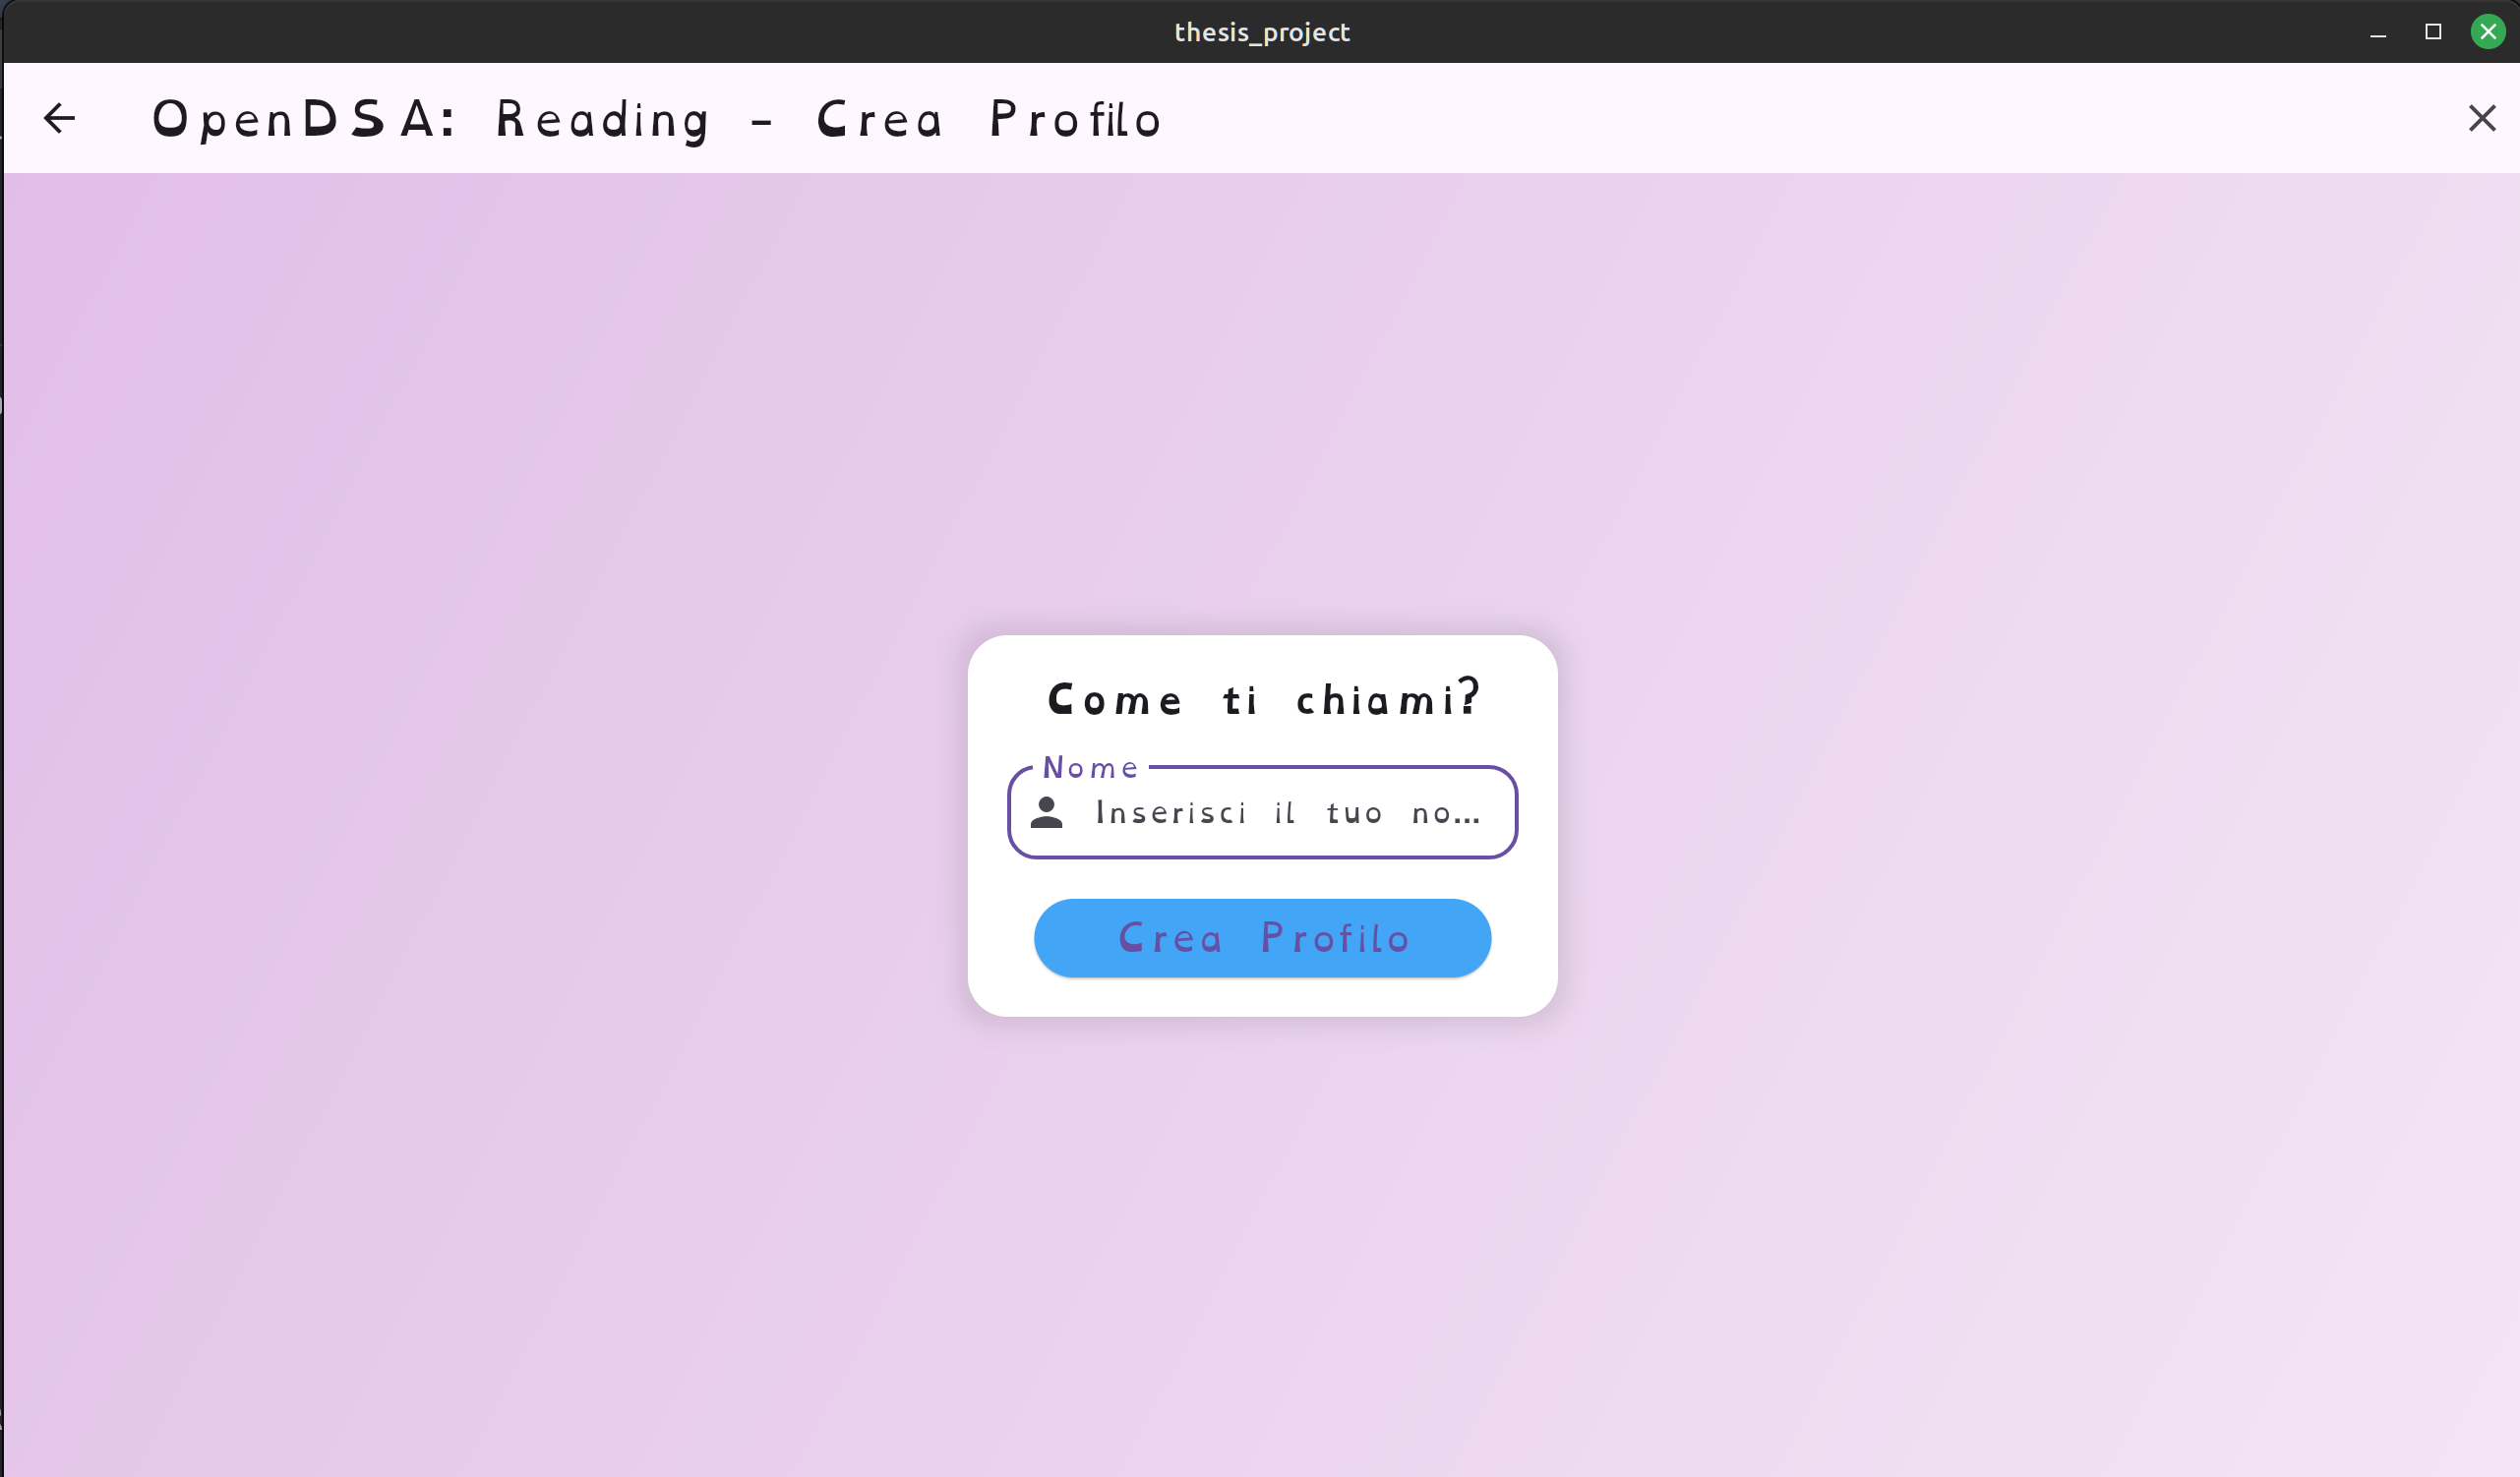
\includegraphics[width=16cm]{Images/0.png}\\
\subsection{La Selezione del Profilo}
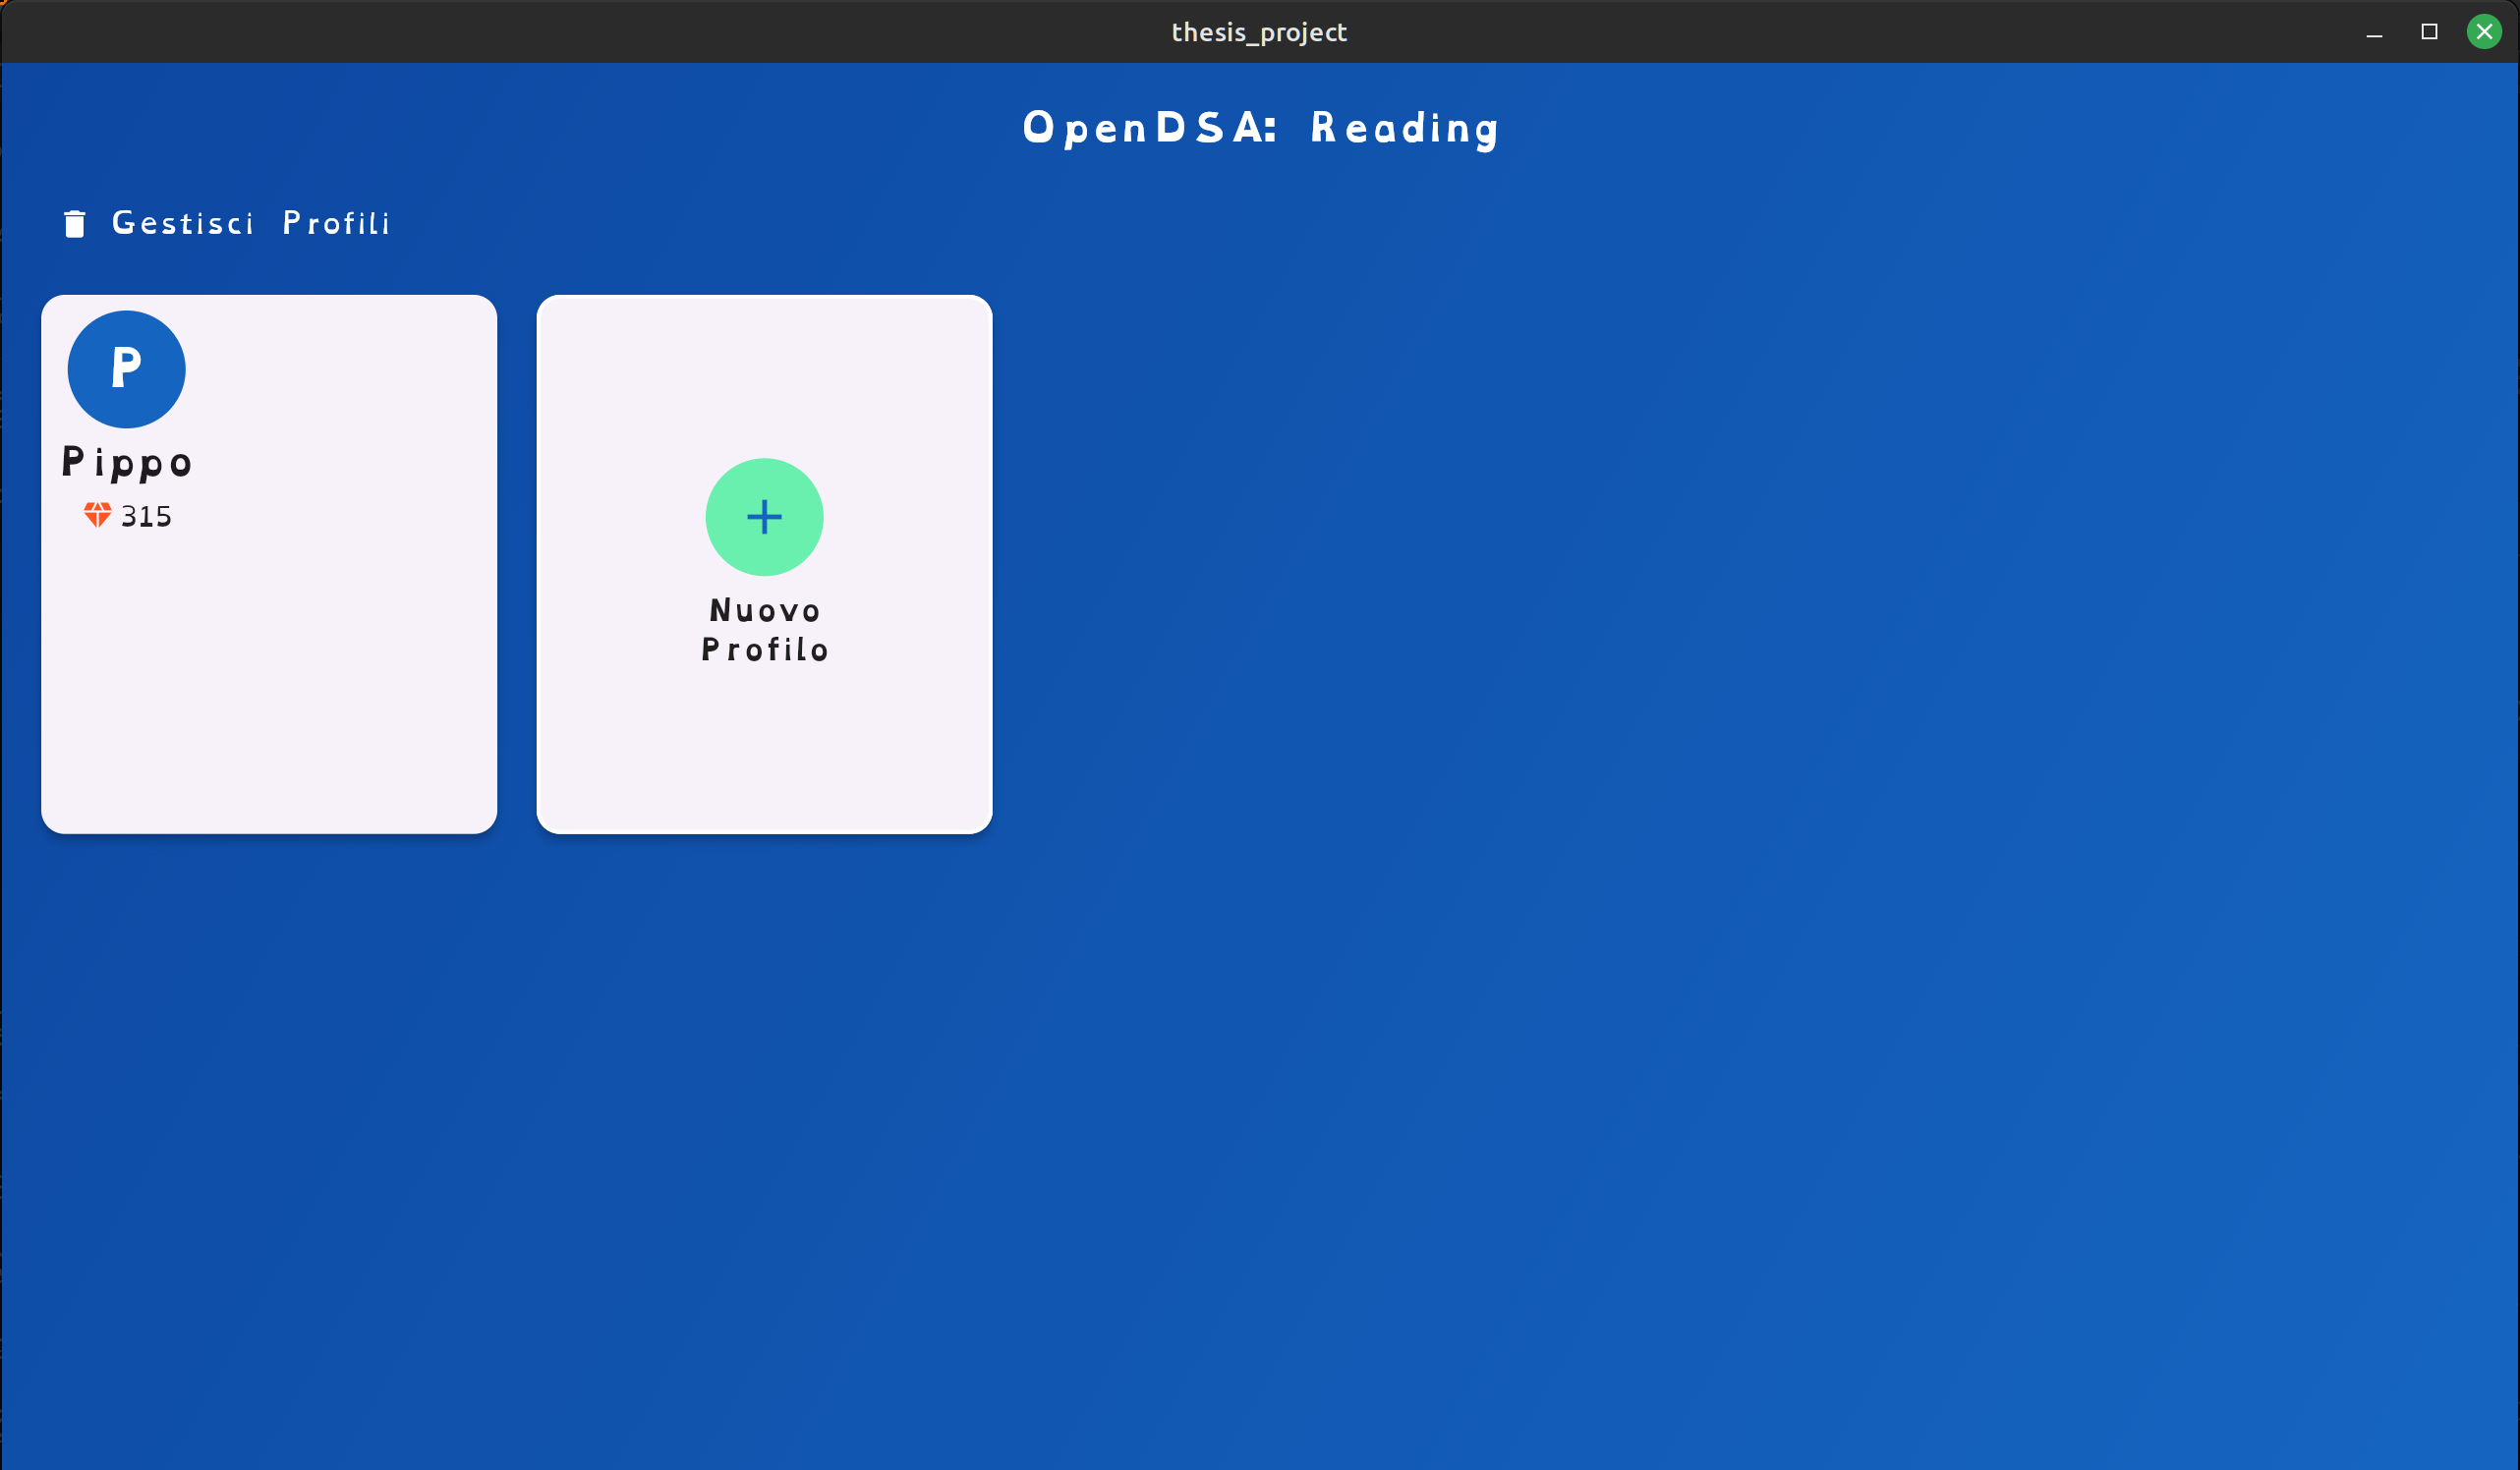
\includegraphics[width=16cm]{Images/1.png}\\
Poiché ho avuto modo di usare l'\textit{Applicazione}, in questo momento è presente il Profilo di prova "Pippo" (nome consueto per i test informatici). Tuttavia, in alto a sinistra, è possibile notare un pulsante "Gestisci Profili", questo pulsante consentirà di abilitare delle piccole checkbox nelle card dei Profili per poterli eventualmente eliminare.\\\\
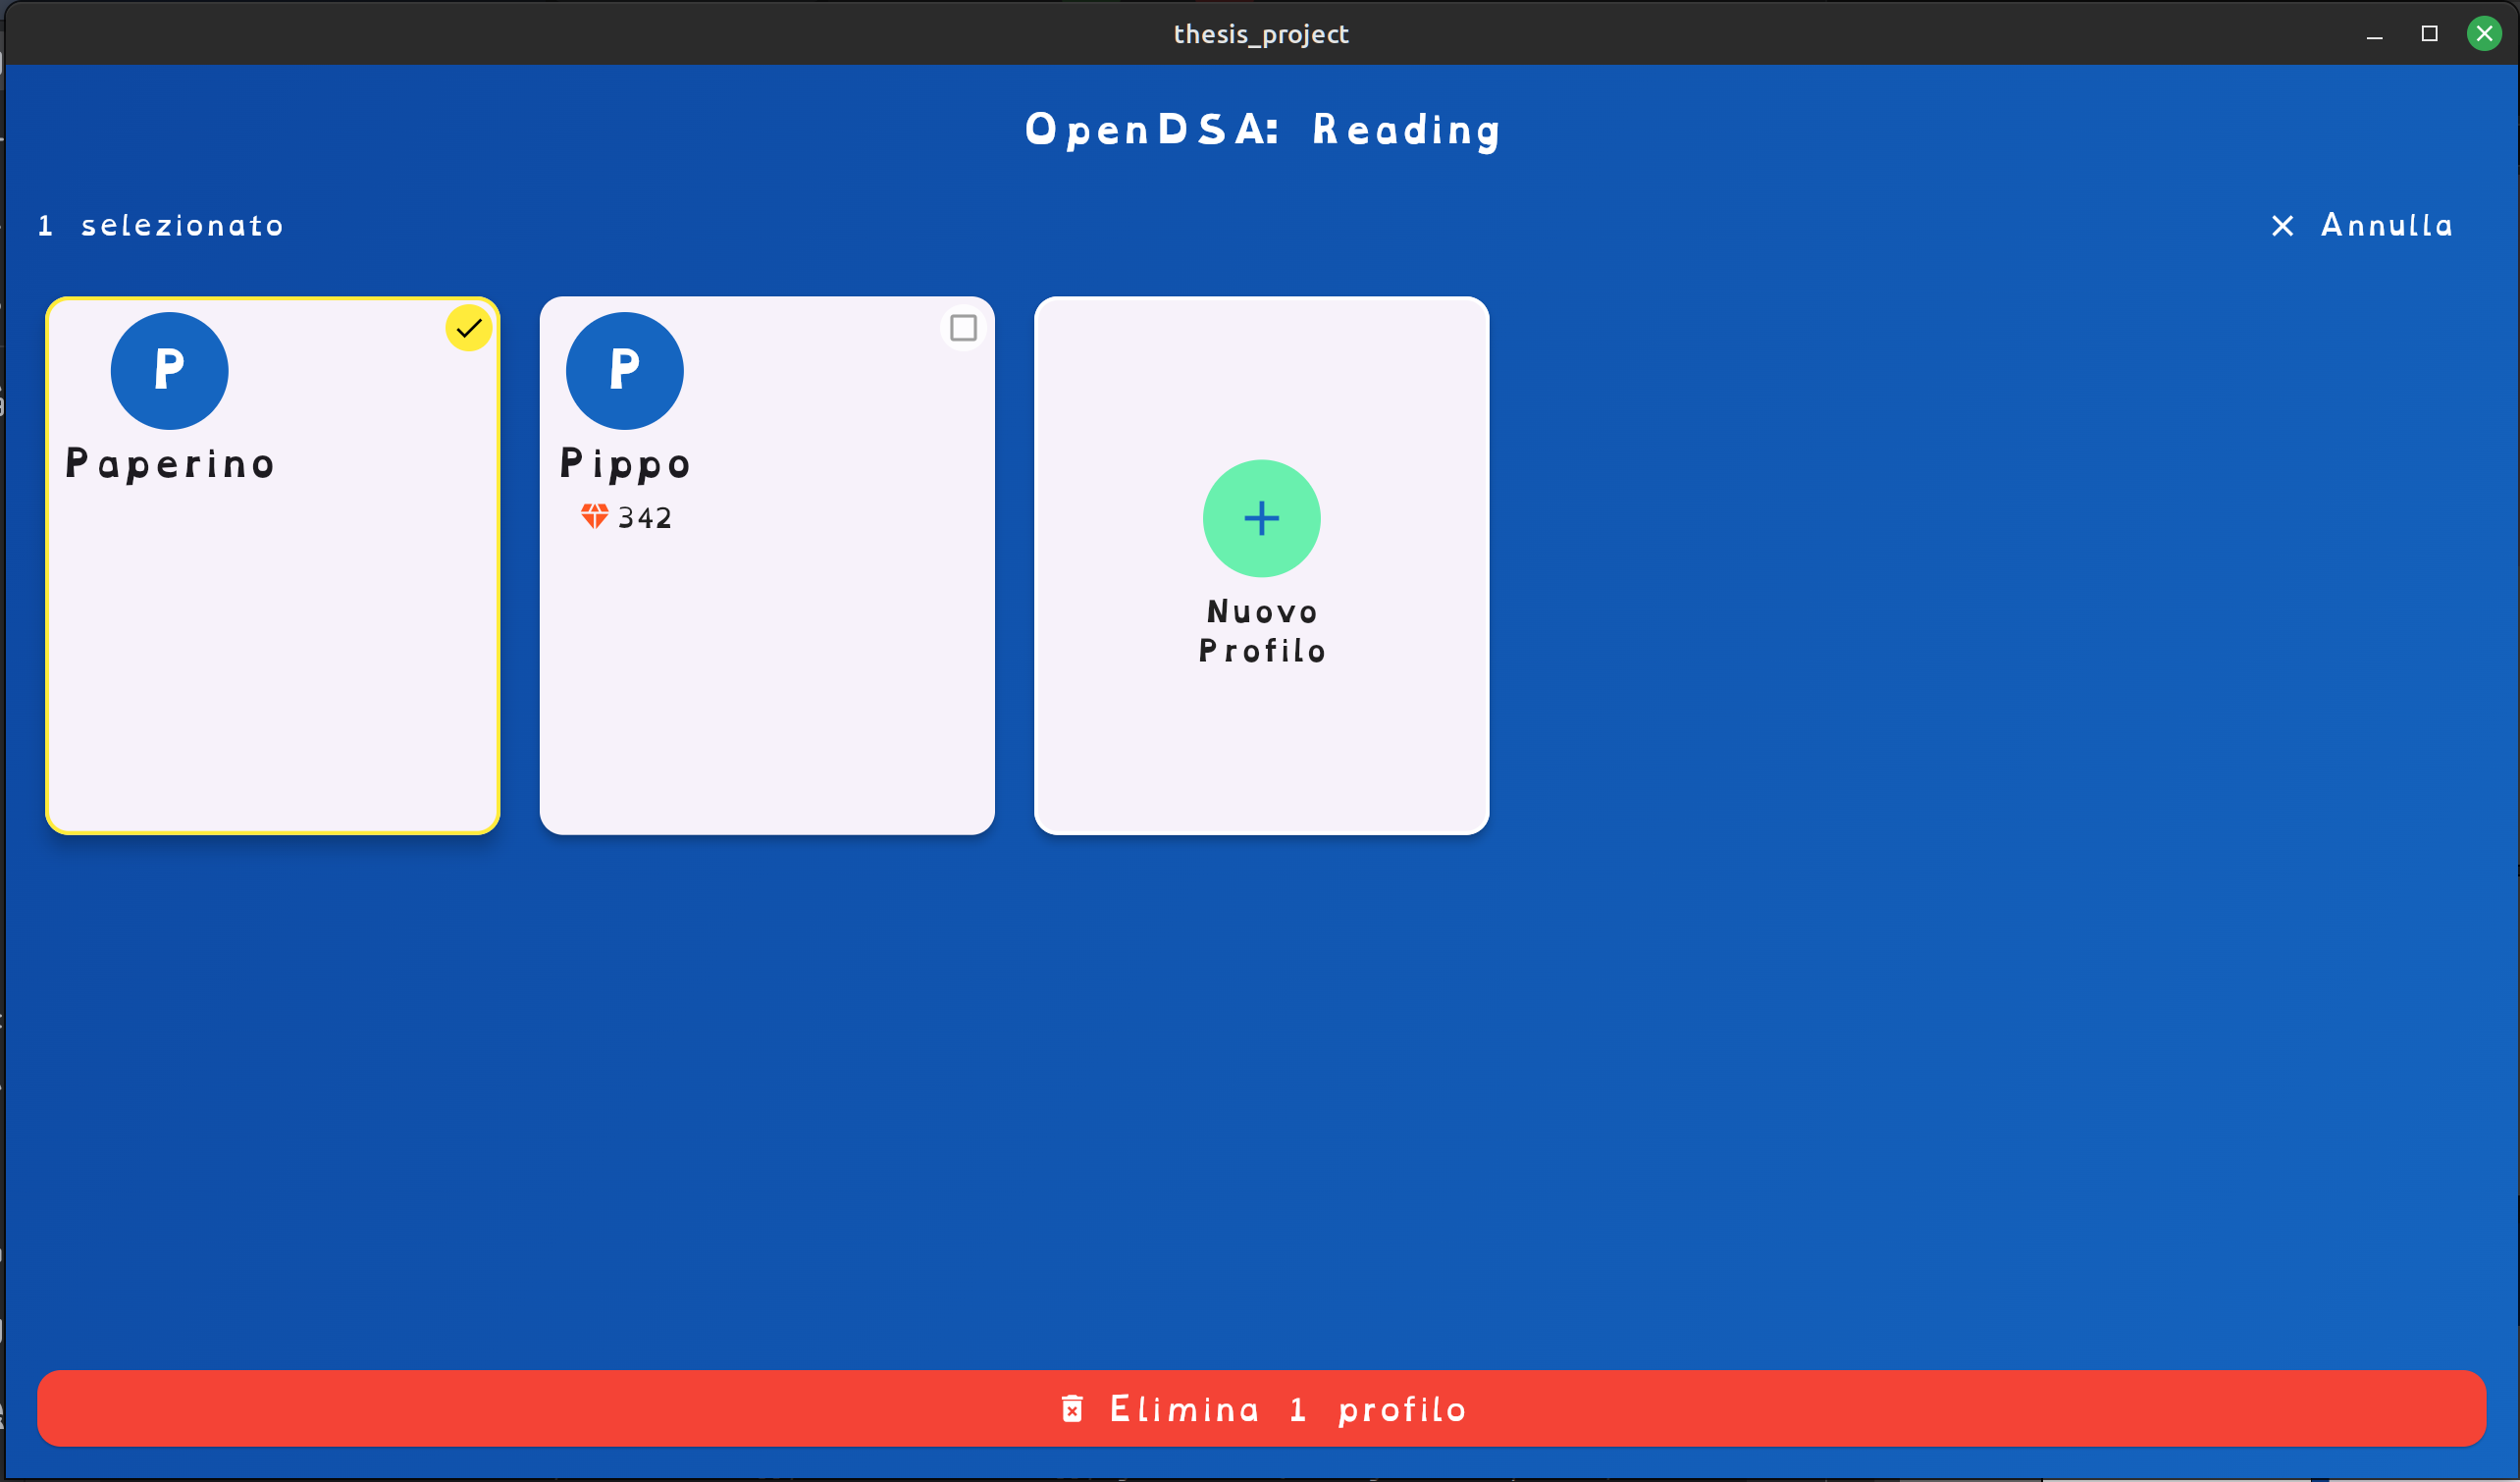
\includegraphics[width=16cm]{Images/0a.png}\\
Alla scelta del Profilo da eliminare, un popup ci intimerà ad accertarci della nostra azione, in quanto irreversibile. Questo meccanismo è stato pernsato per prevenire eventuali errori o per gestire eventuali ripensamenti che l'utente potrebbe avere nella User Journey della App. \\\\
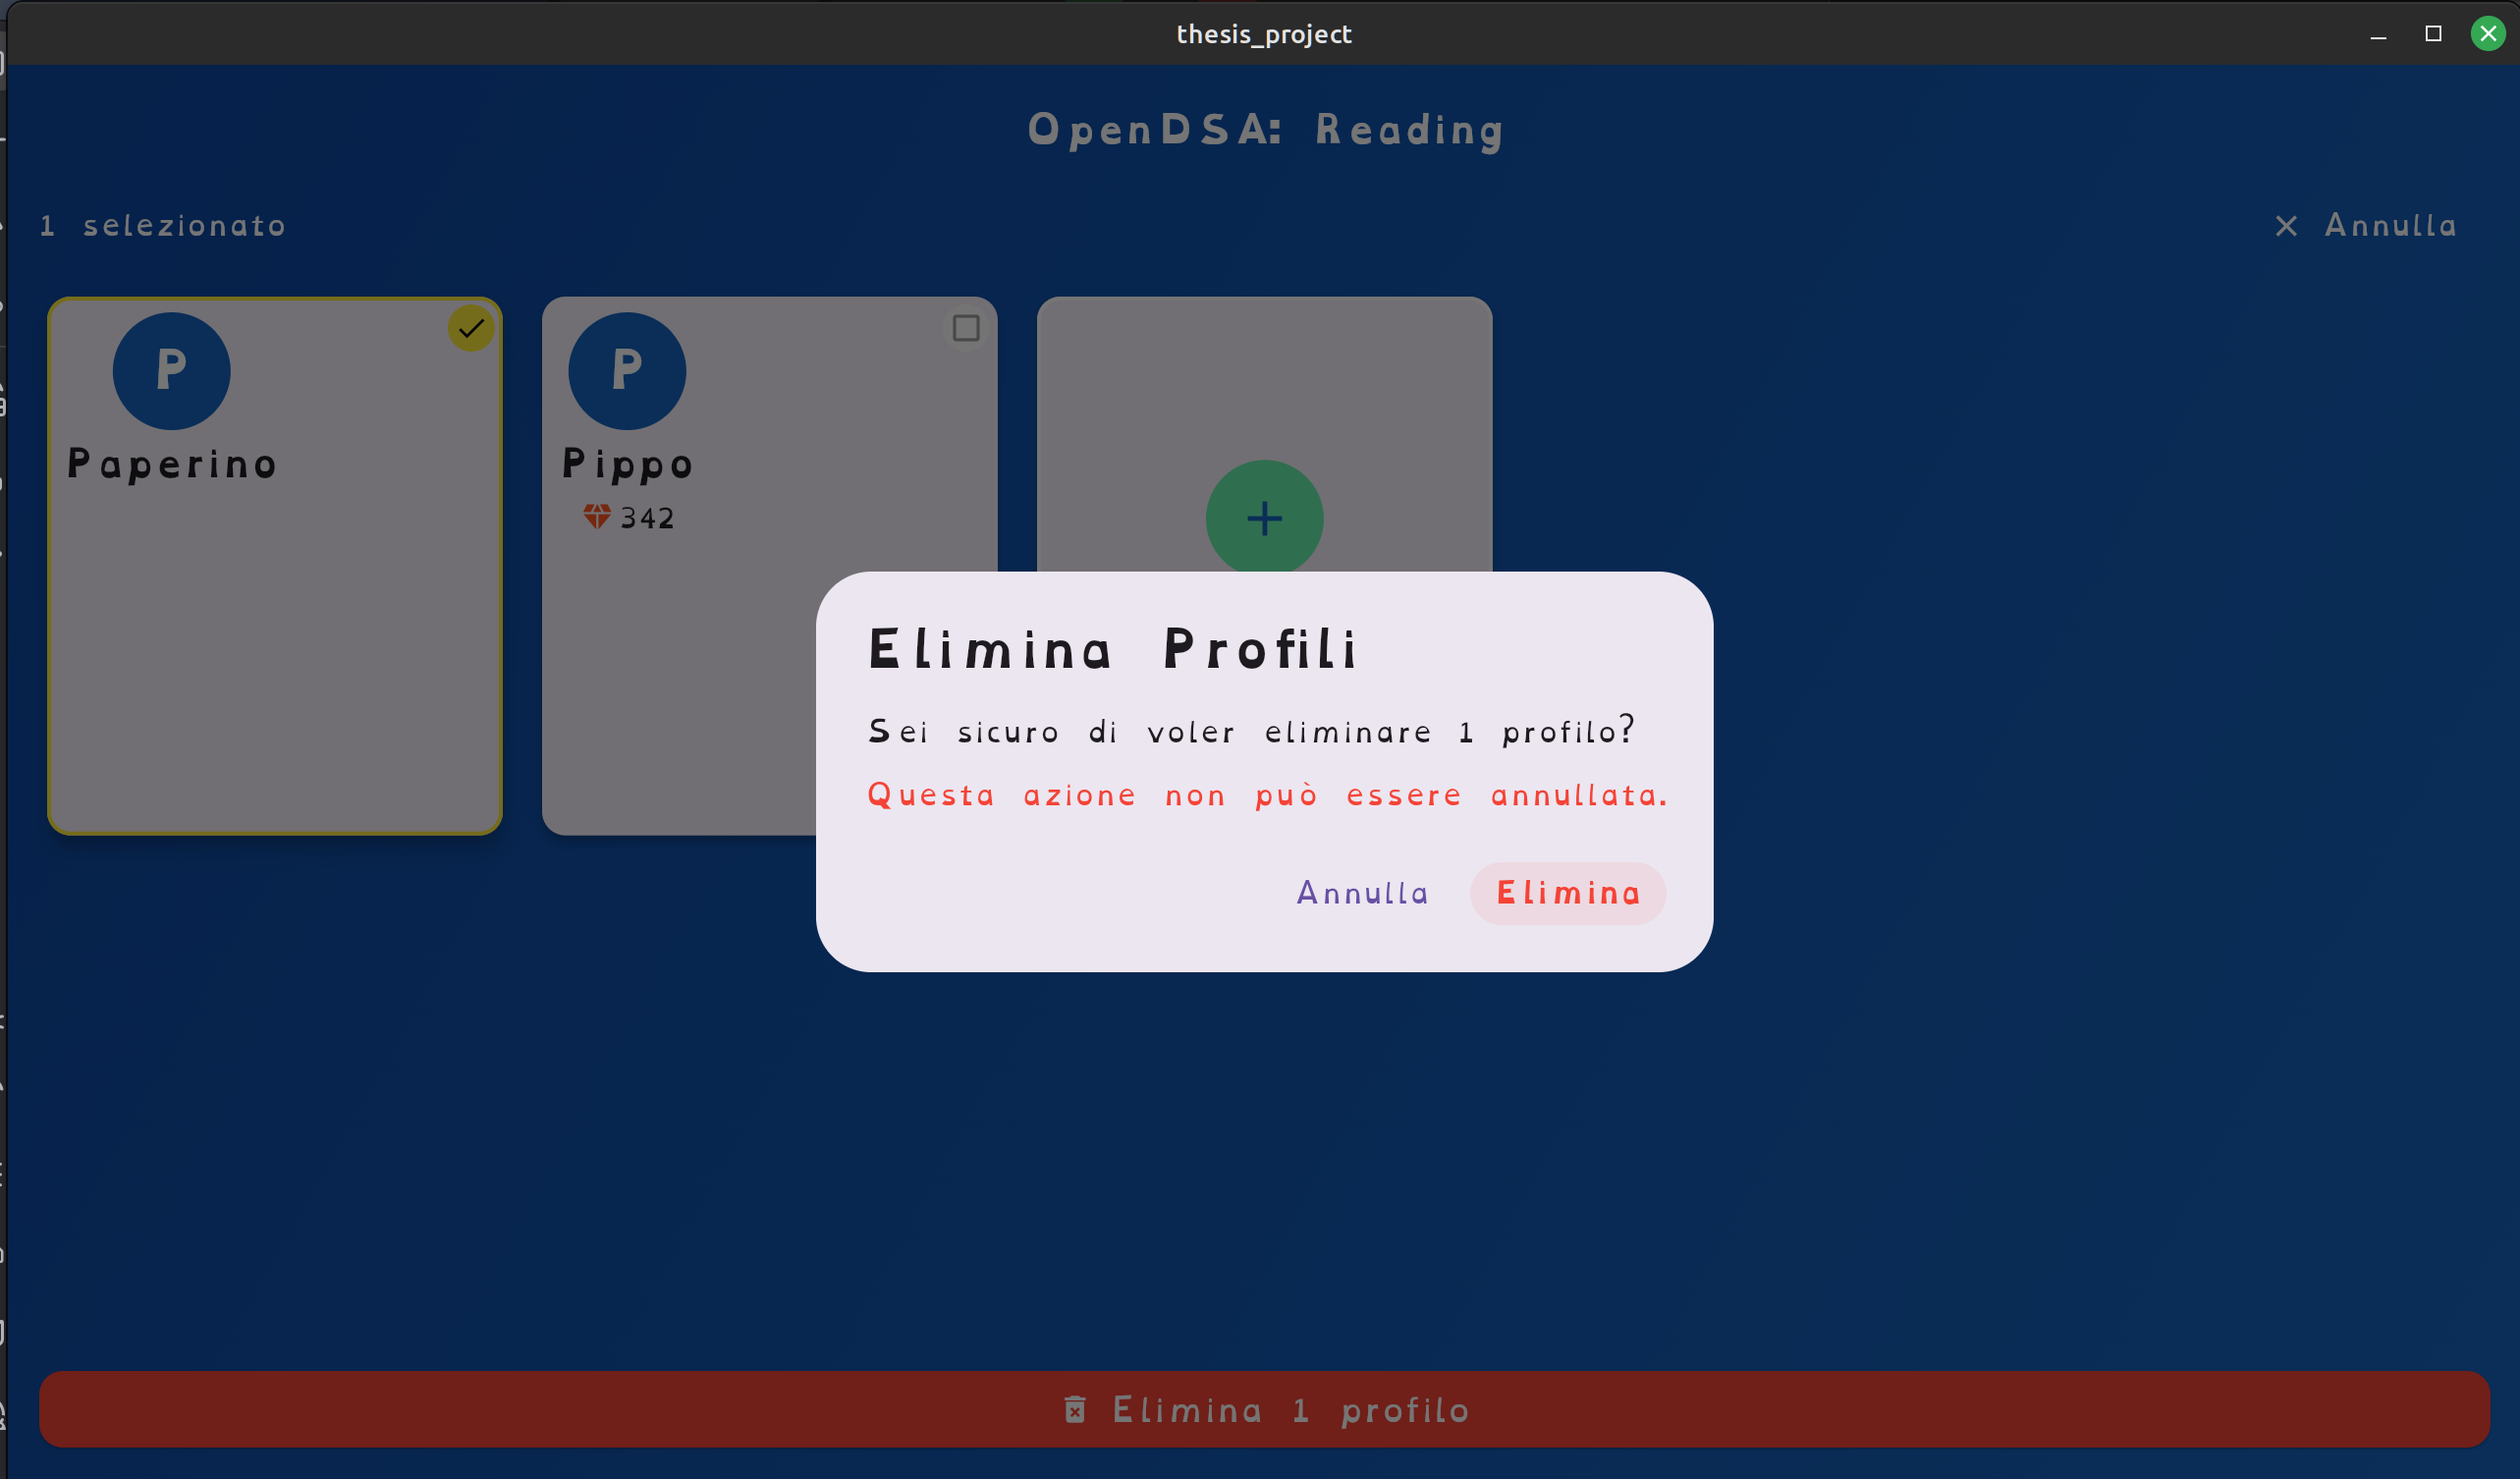
\includegraphics[width=16cm]{Images/0b.png}\\
Una volta deciso di voler giocare, verremo catapultati all'interno della \textit{Schermata di Gioco}, con il riepilogo del nostro \textit{Profilo} (Obiettivi da raggiungere, Cristalli accumulati, barra di progressione del Livello, numero di giorni per cui abbiamo giocato, Progresso delle nostre sfide, ecc). La schermata è piuttosto intuitiva e colorata per dare enfasi alle varie sfaccettature del gioco.\\\\
\subsection{La Schermata di Gioco Principale}
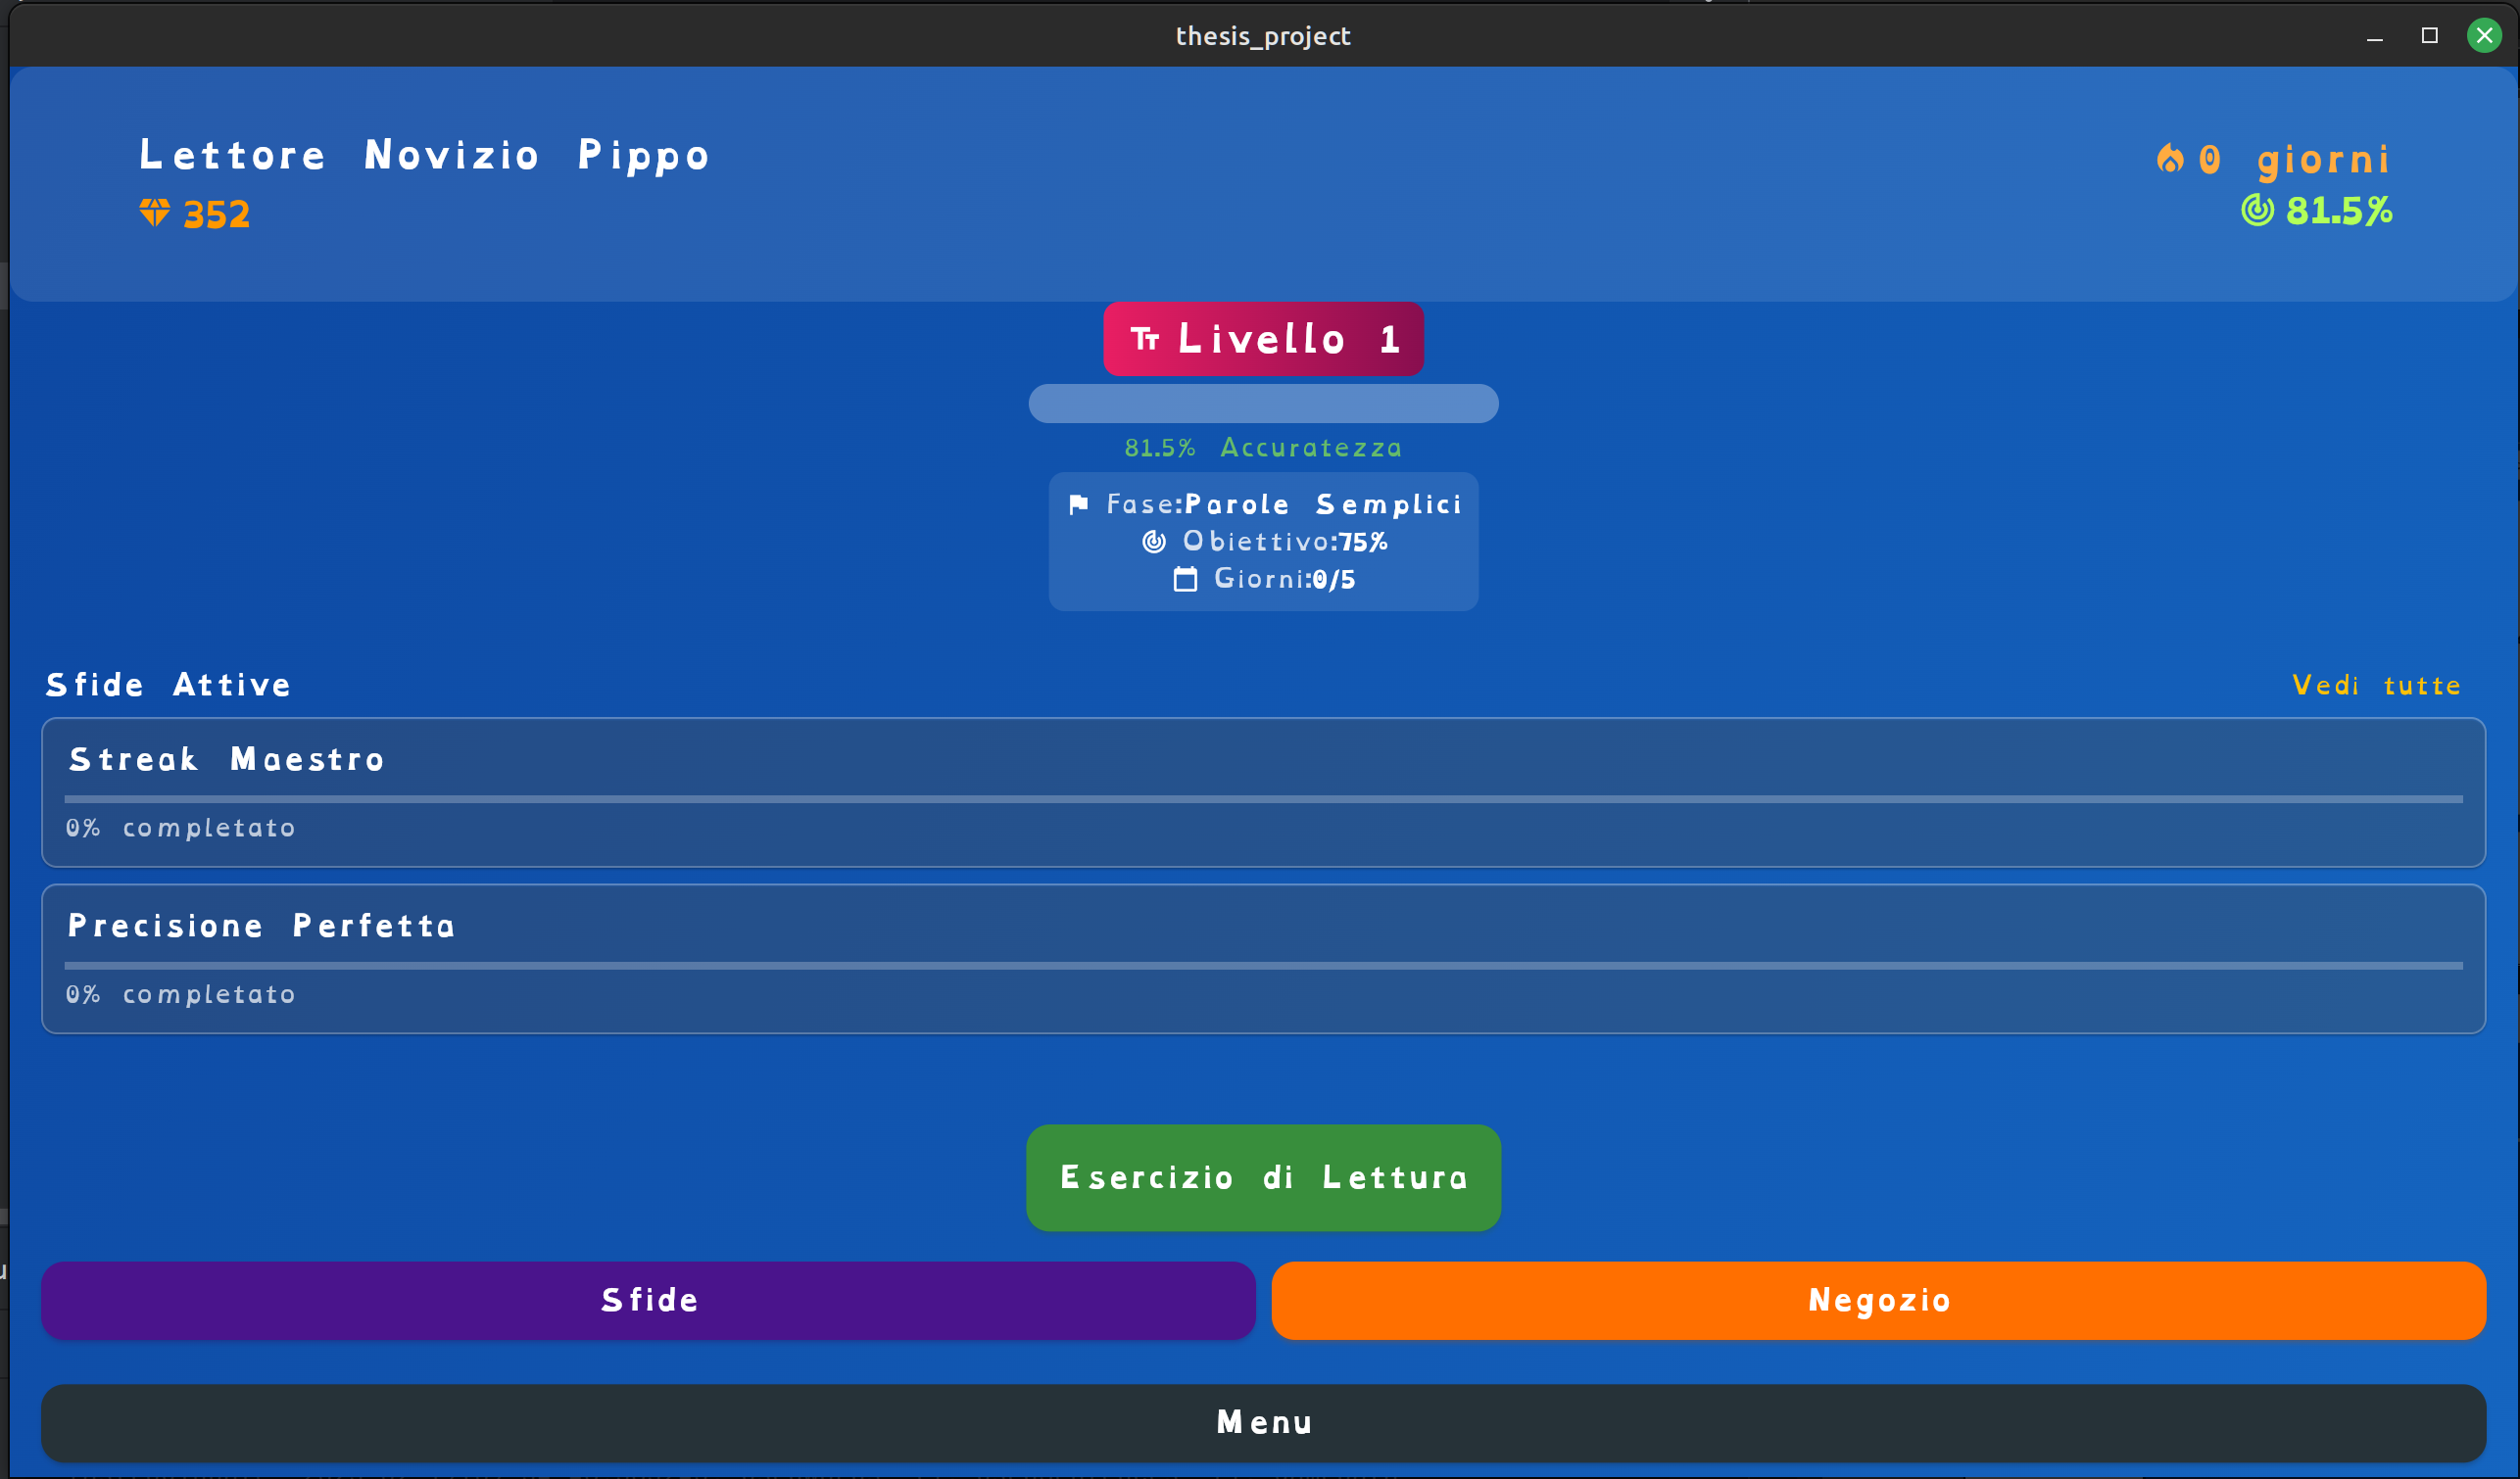
\includegraphics[width=16cm]{Images/2.png}\\
Attraverso il pulsante "Sfide" potremo accedere alla prima parte della struttura di Gamification implementata, che aiuterà a mantenere alto l'interesse verso l'uso della app (l'obiettivo delle sfide è autoesplicativo). \\\\
\subsection{Le Sfide}
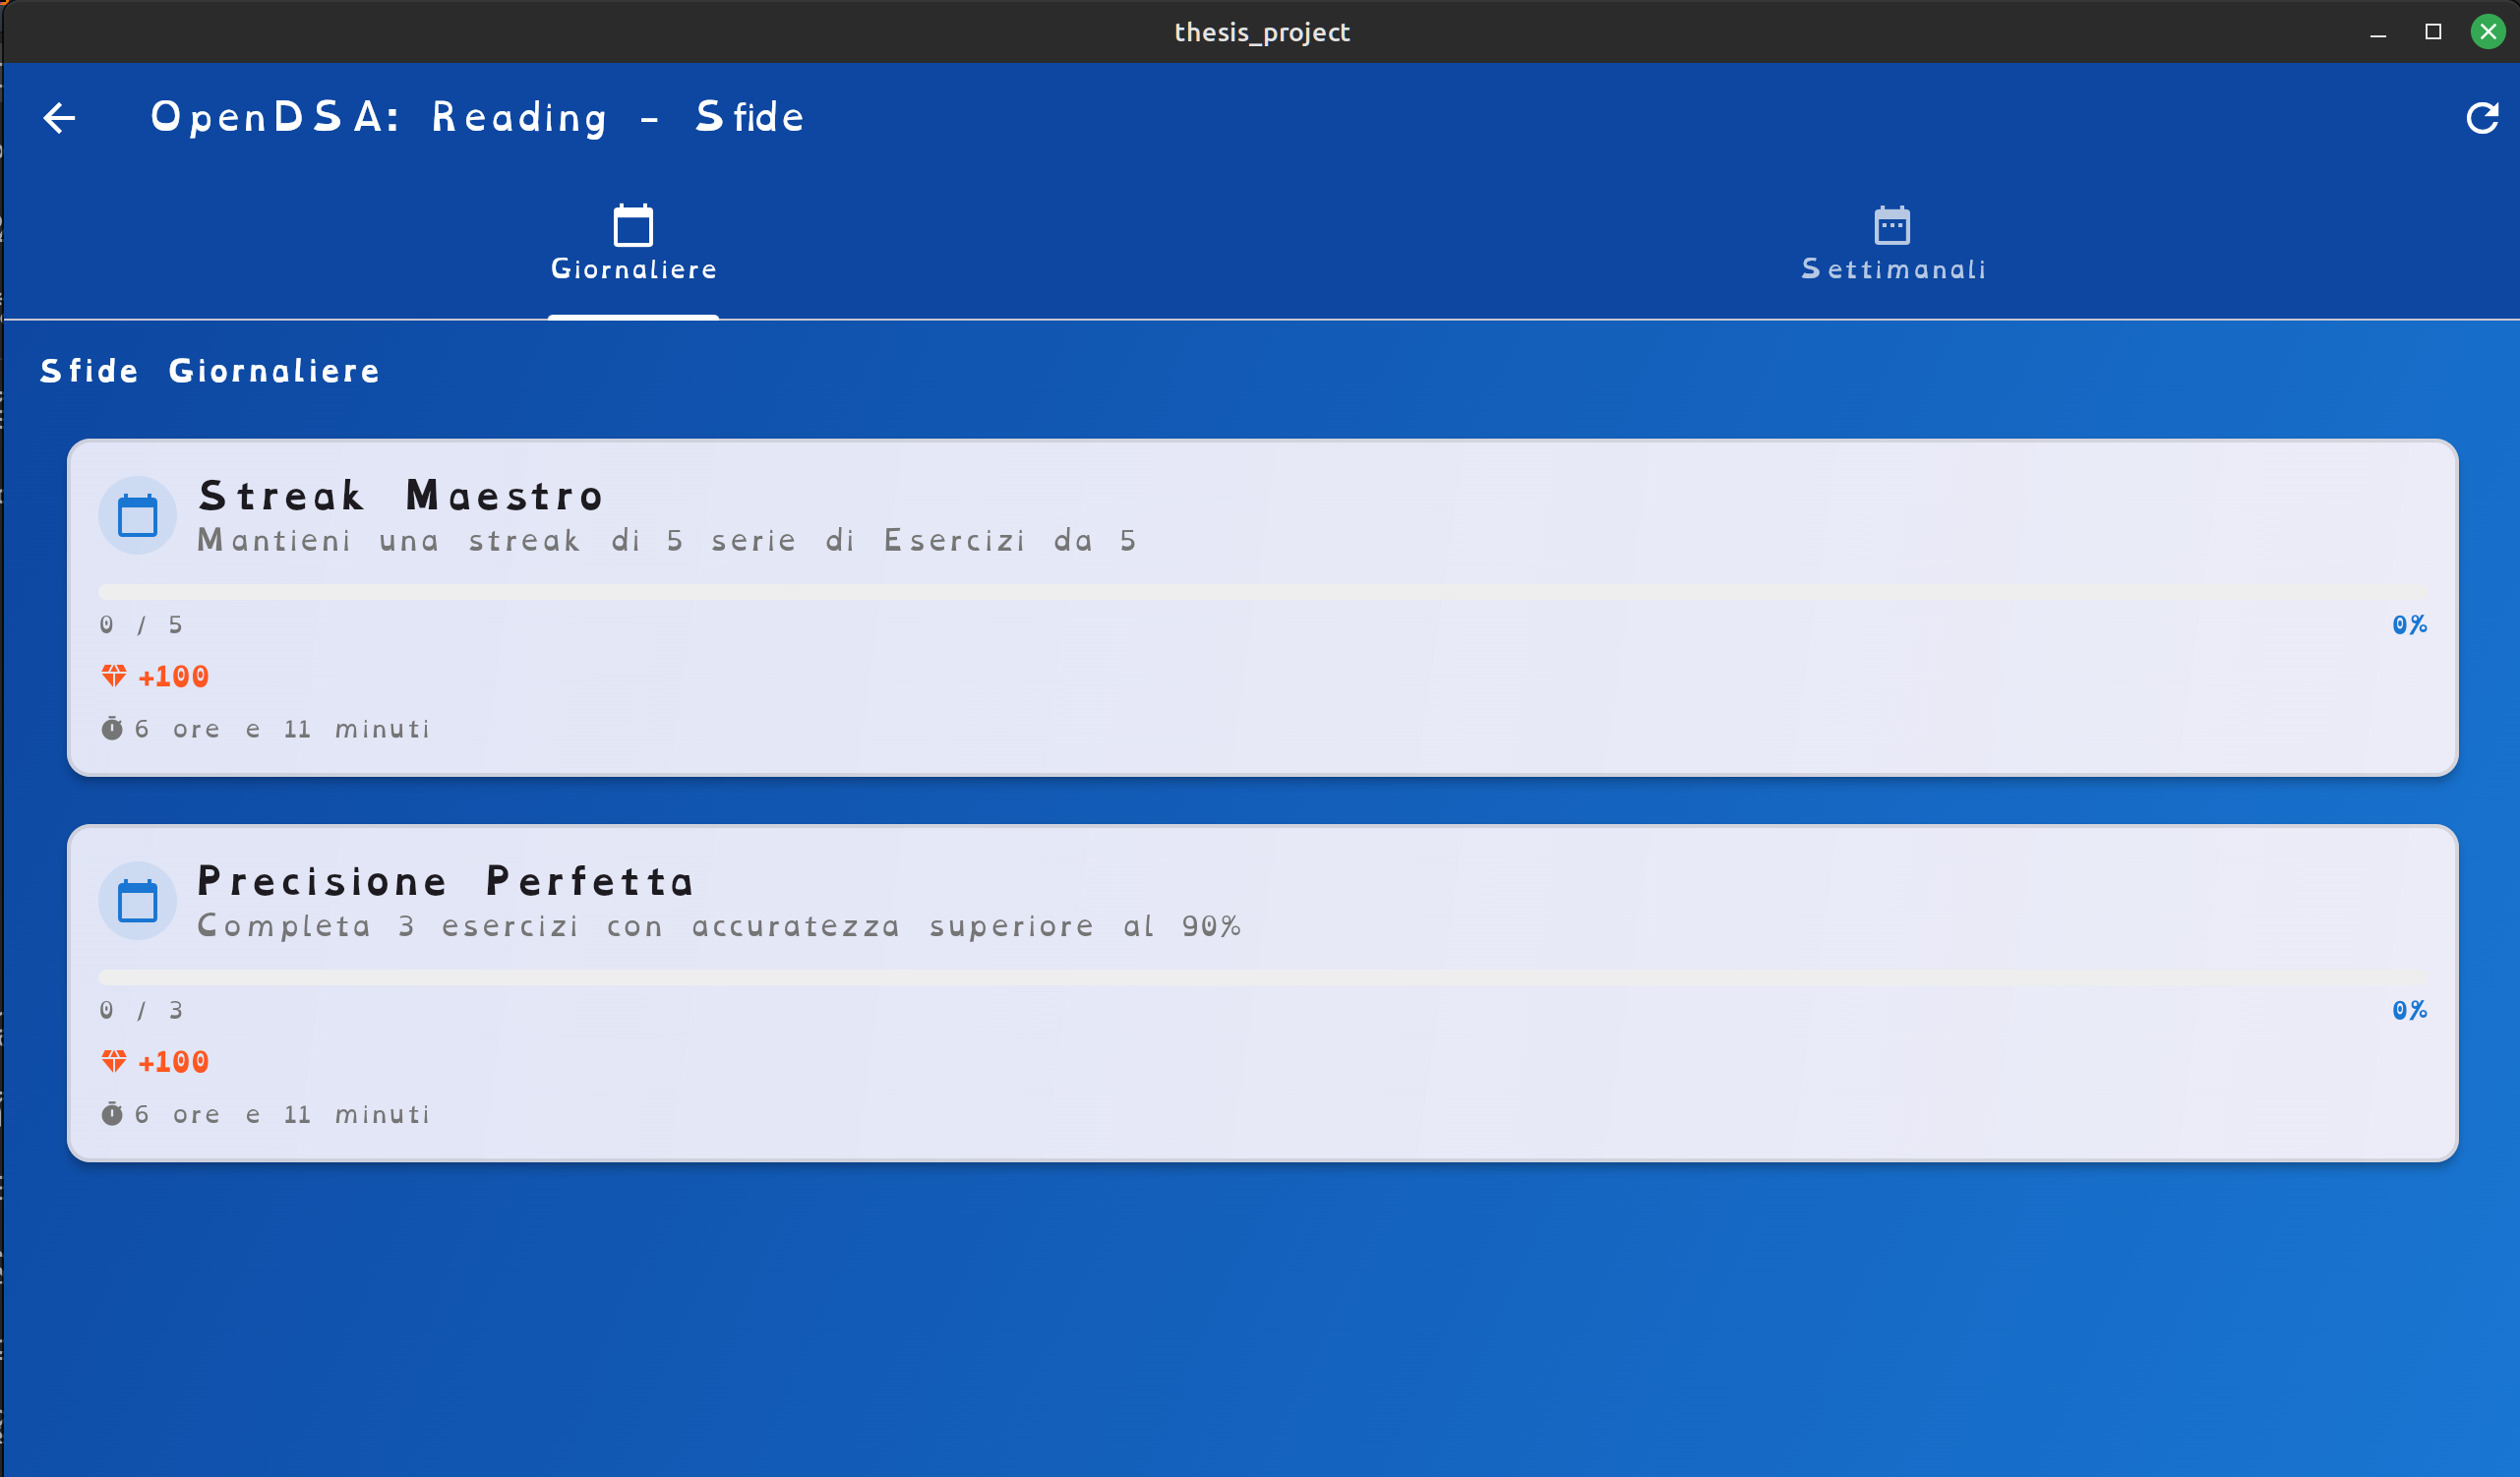
\includegraphics[width=16cm]{Images/3.png}\\
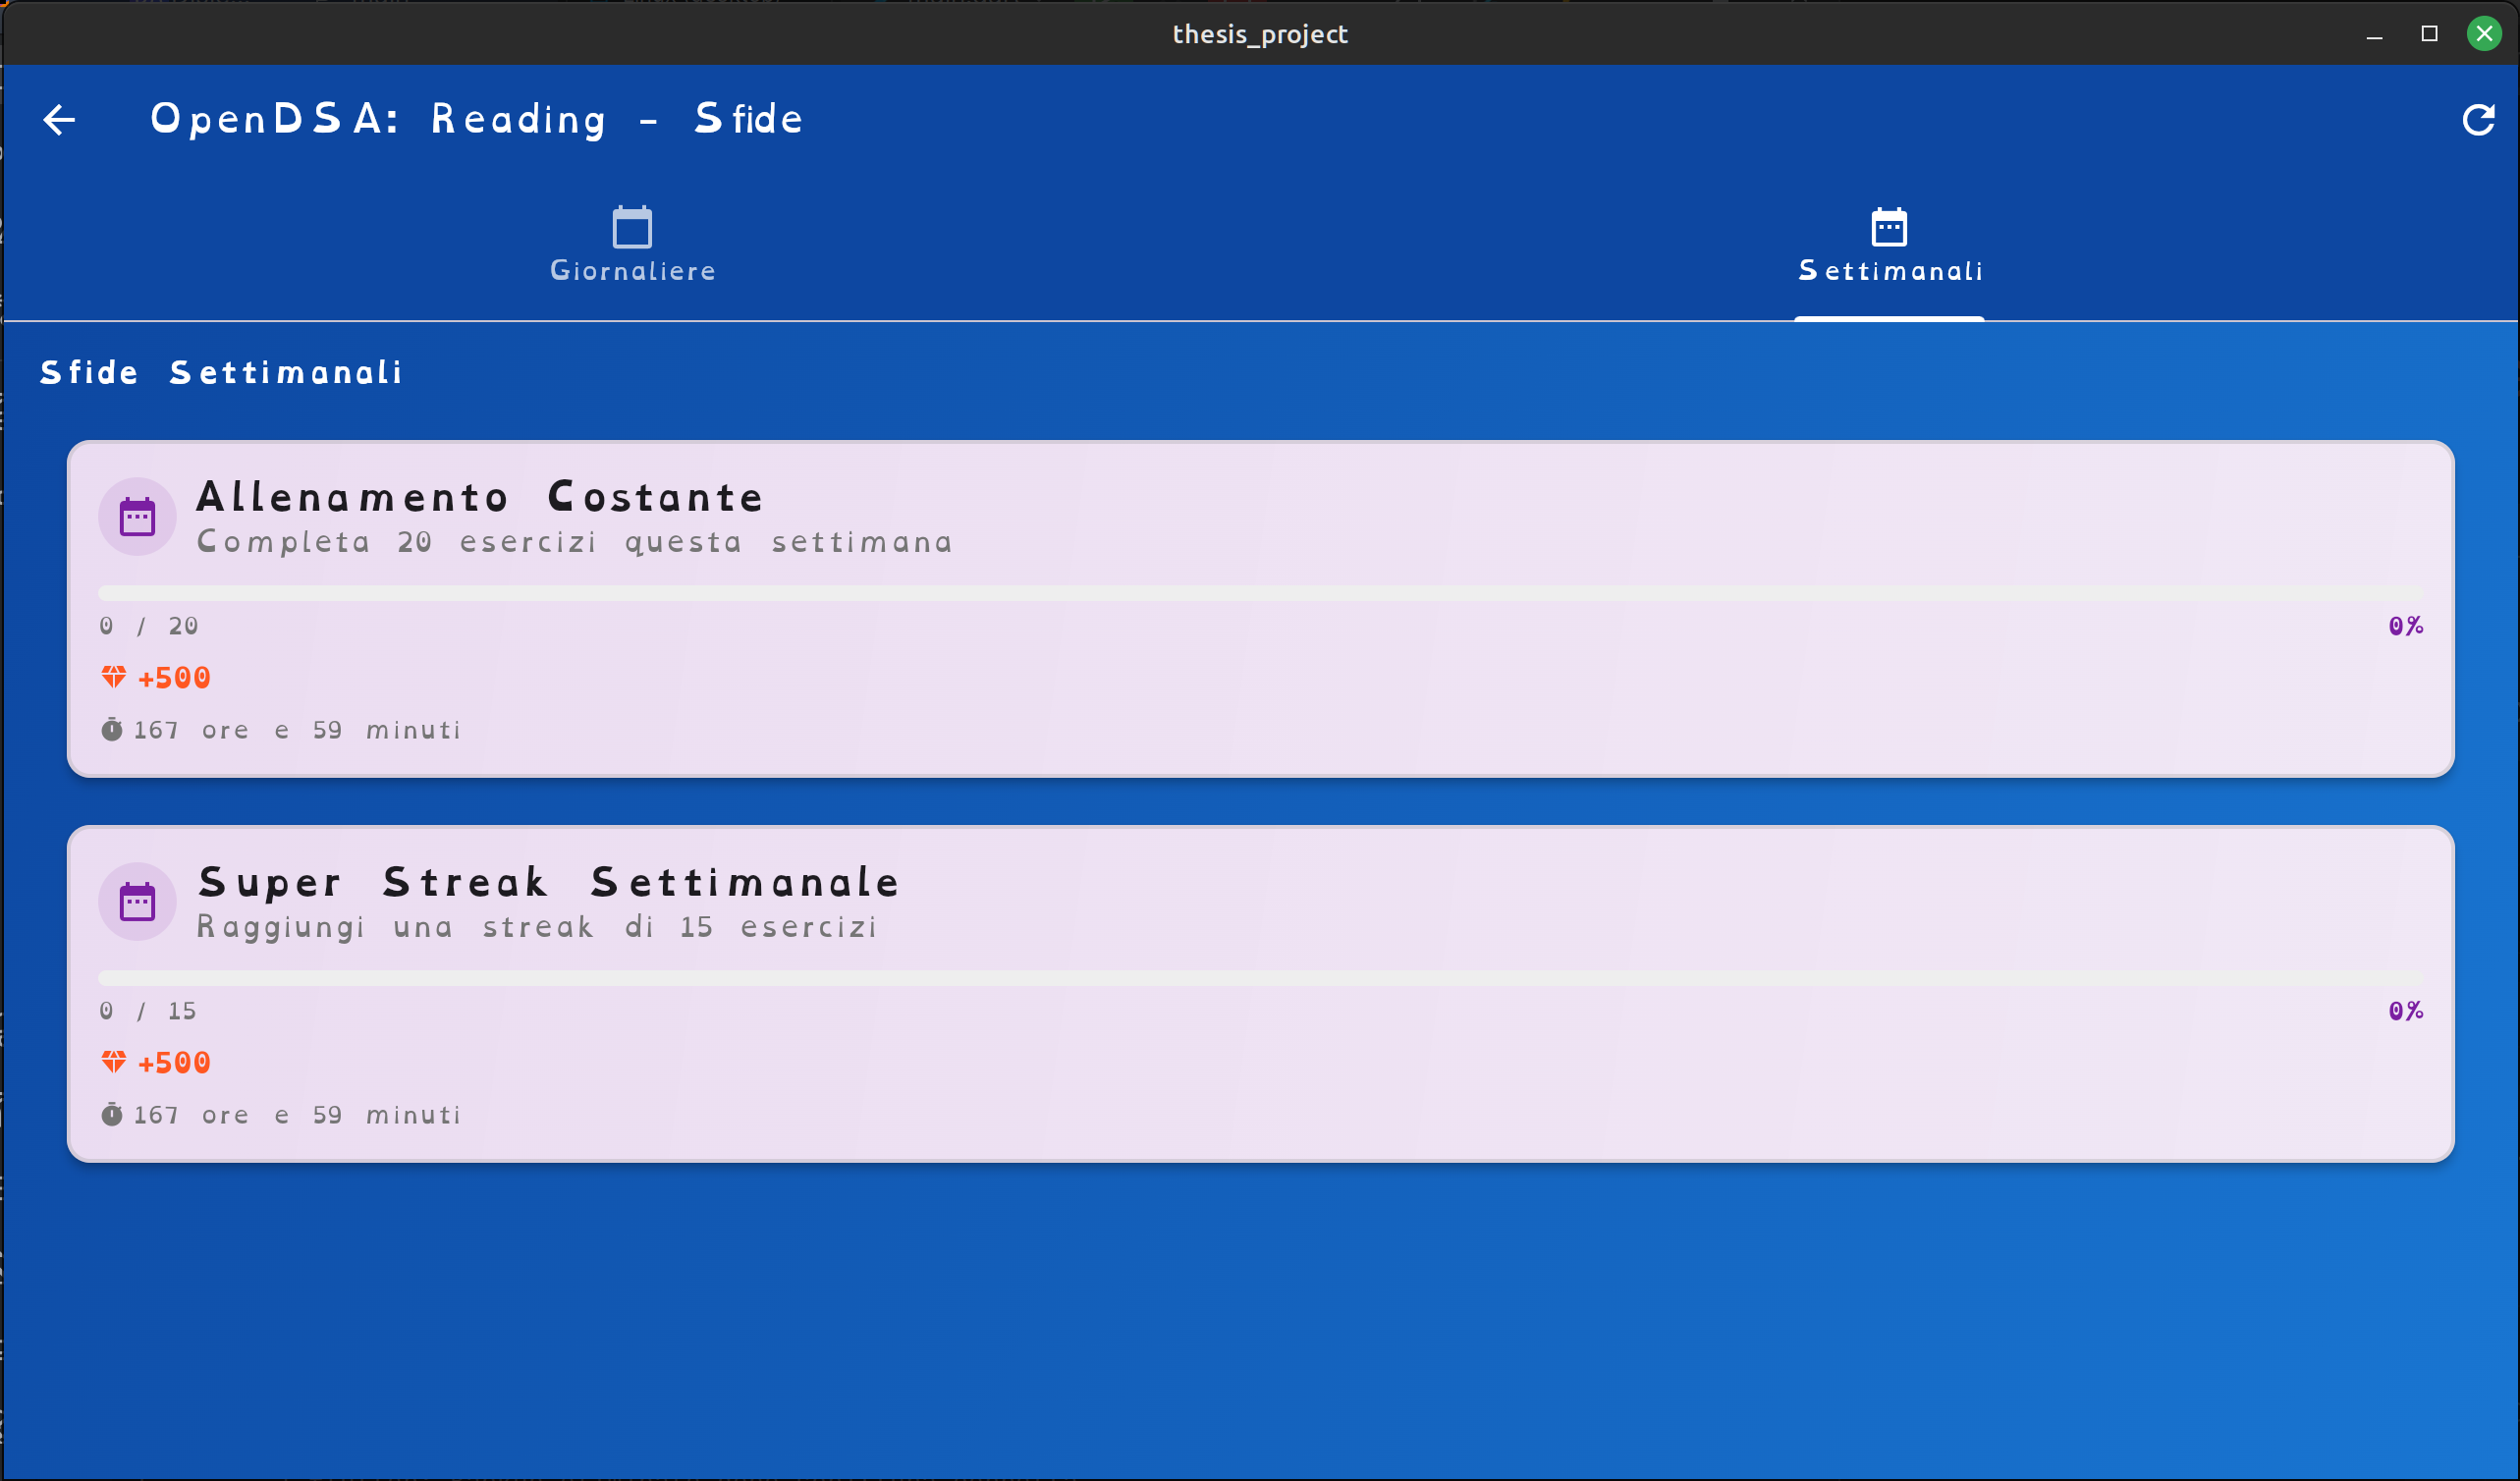
\includegraphics[width=16cm]{Images/4.png}\\
\subsection{I Trofei}
Se decidessimo di entrare nello \textit{Store dei Trofei} invece, possiamo notare le fantasiose e colorate \textit{Card dei Titoli} che possiamo acquistare. Di fatti, il \textit{Titolo} si andrà a sostituire all'attuale \textit{"Lettore Novizio"} con titoli più entusiasmanti che potranno essere comprati attraverso i cristalli accumulati nelle varie sessioni di gioco. \\\\
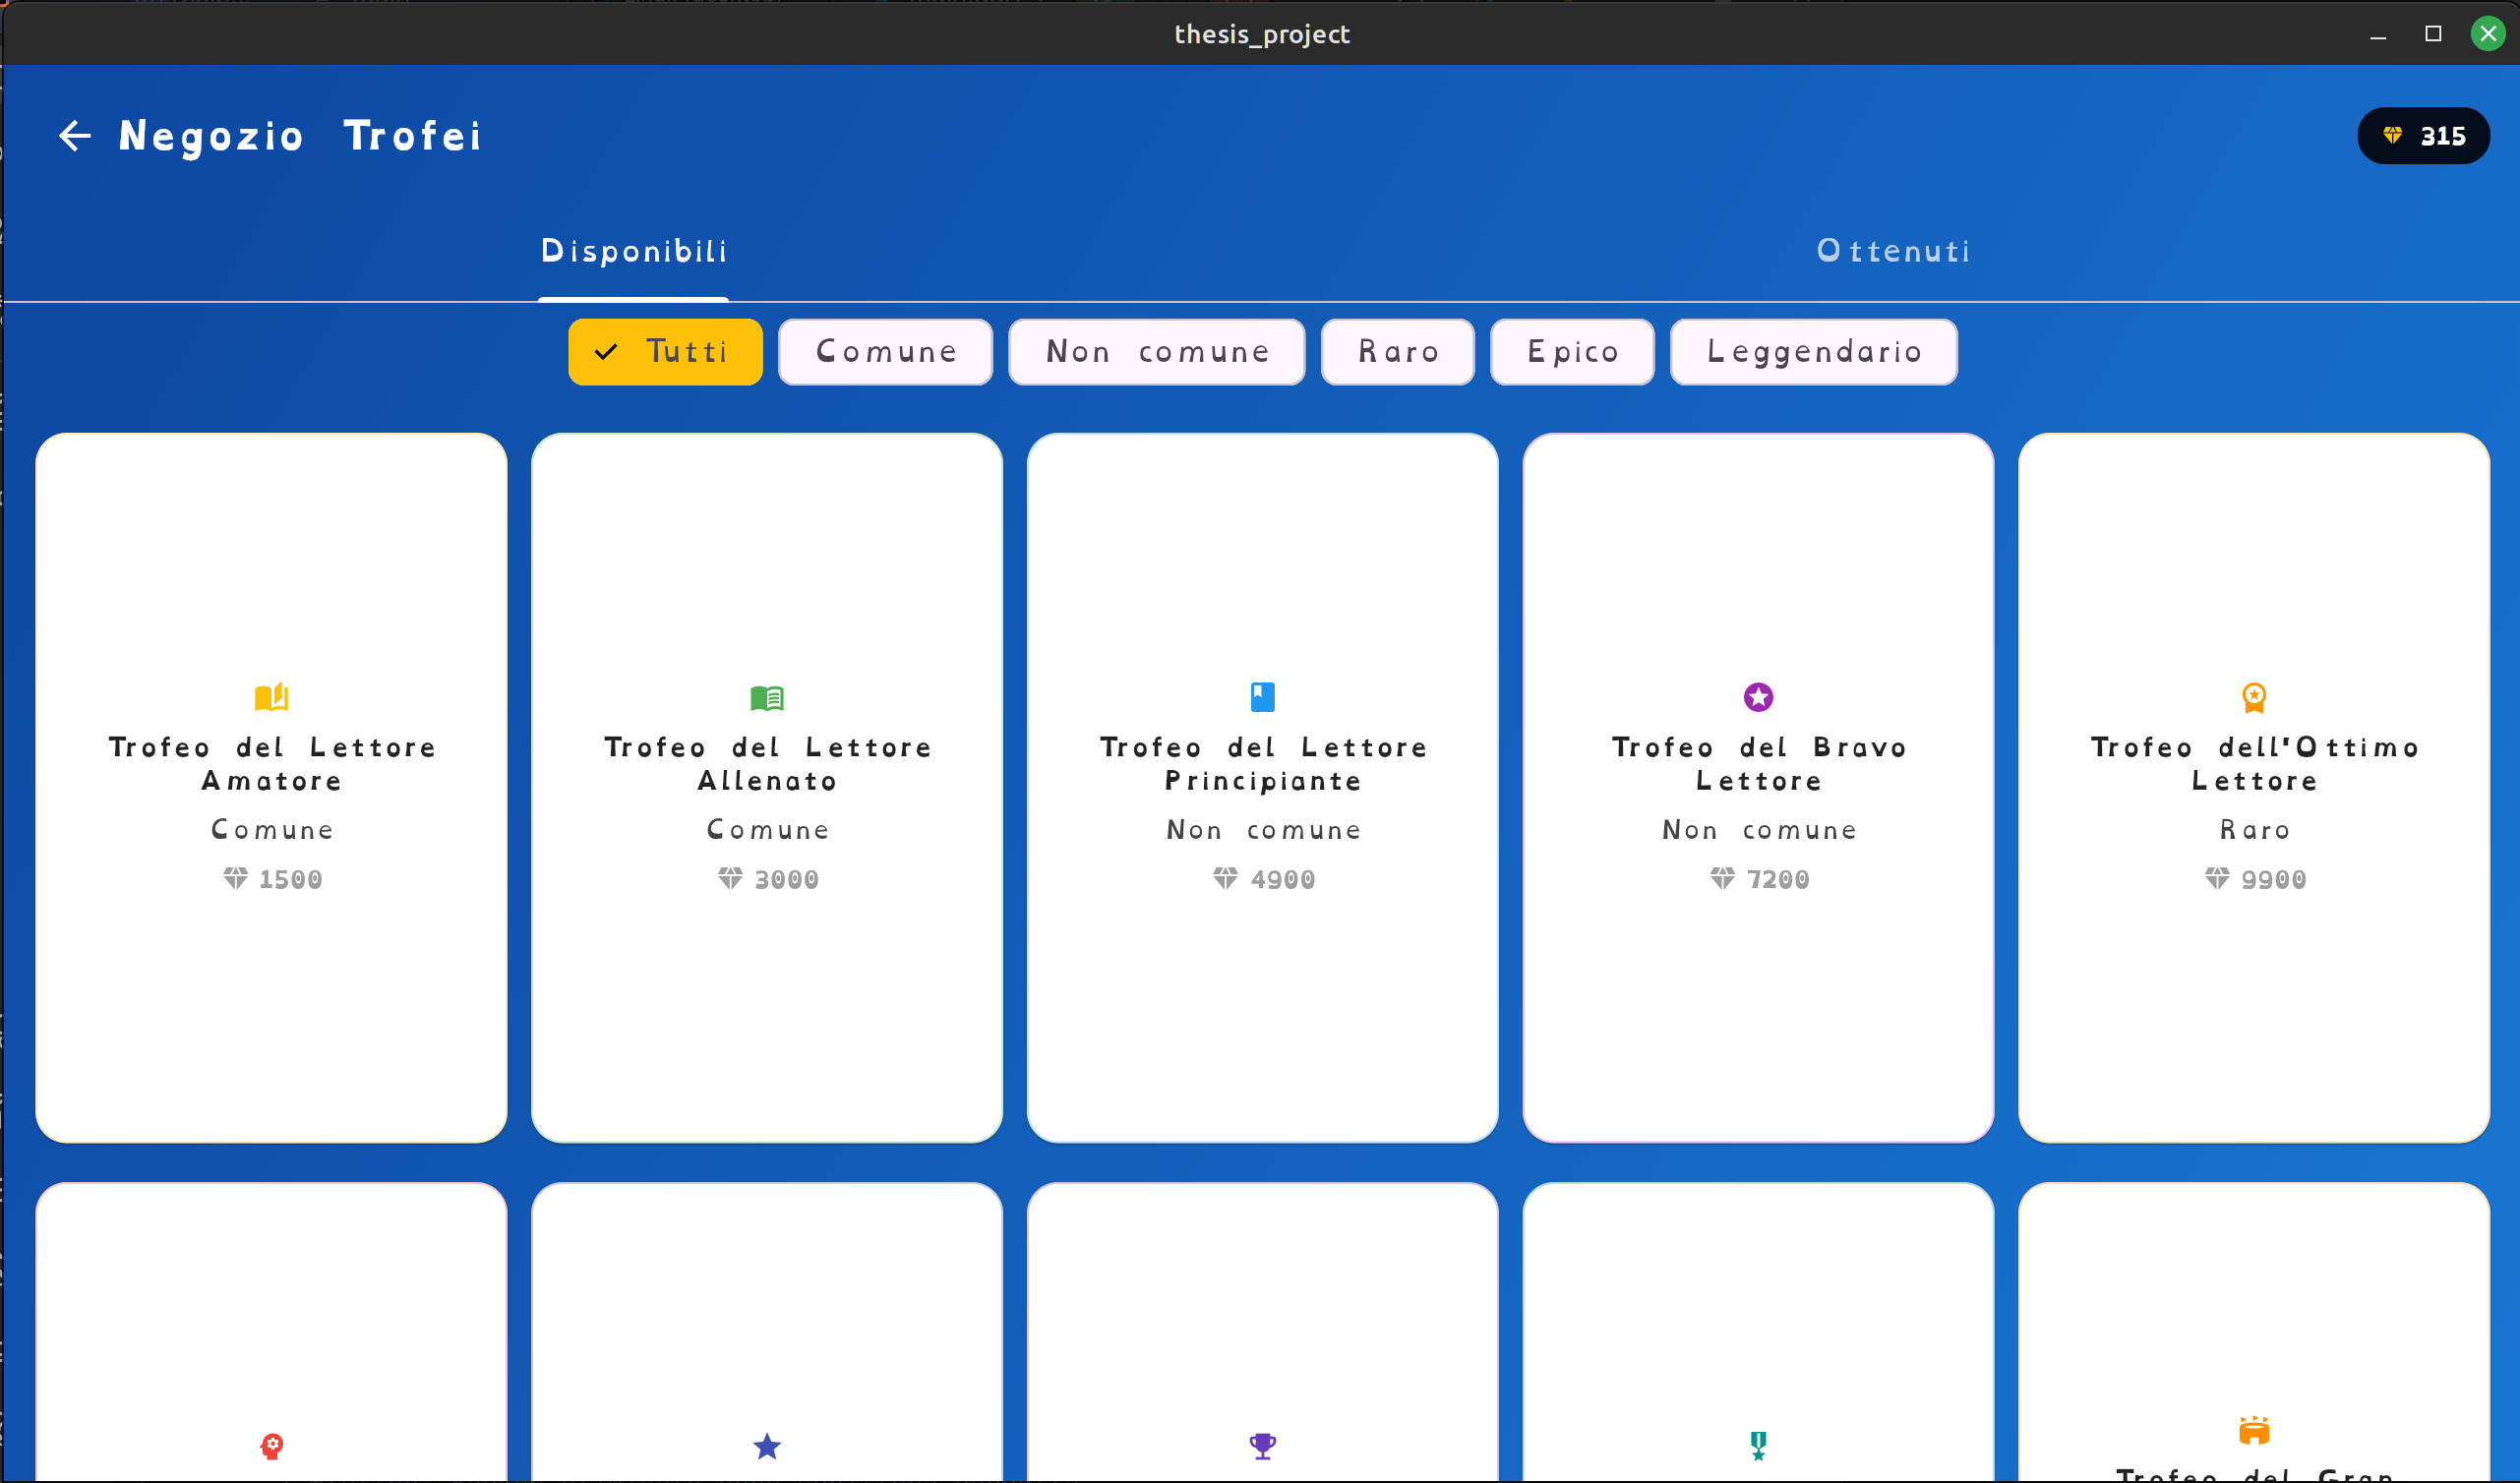
\includegraphics[width=16cm]{Images/5.png}\\
\pagebreak

\subsection{Avvio degli Esercizi}
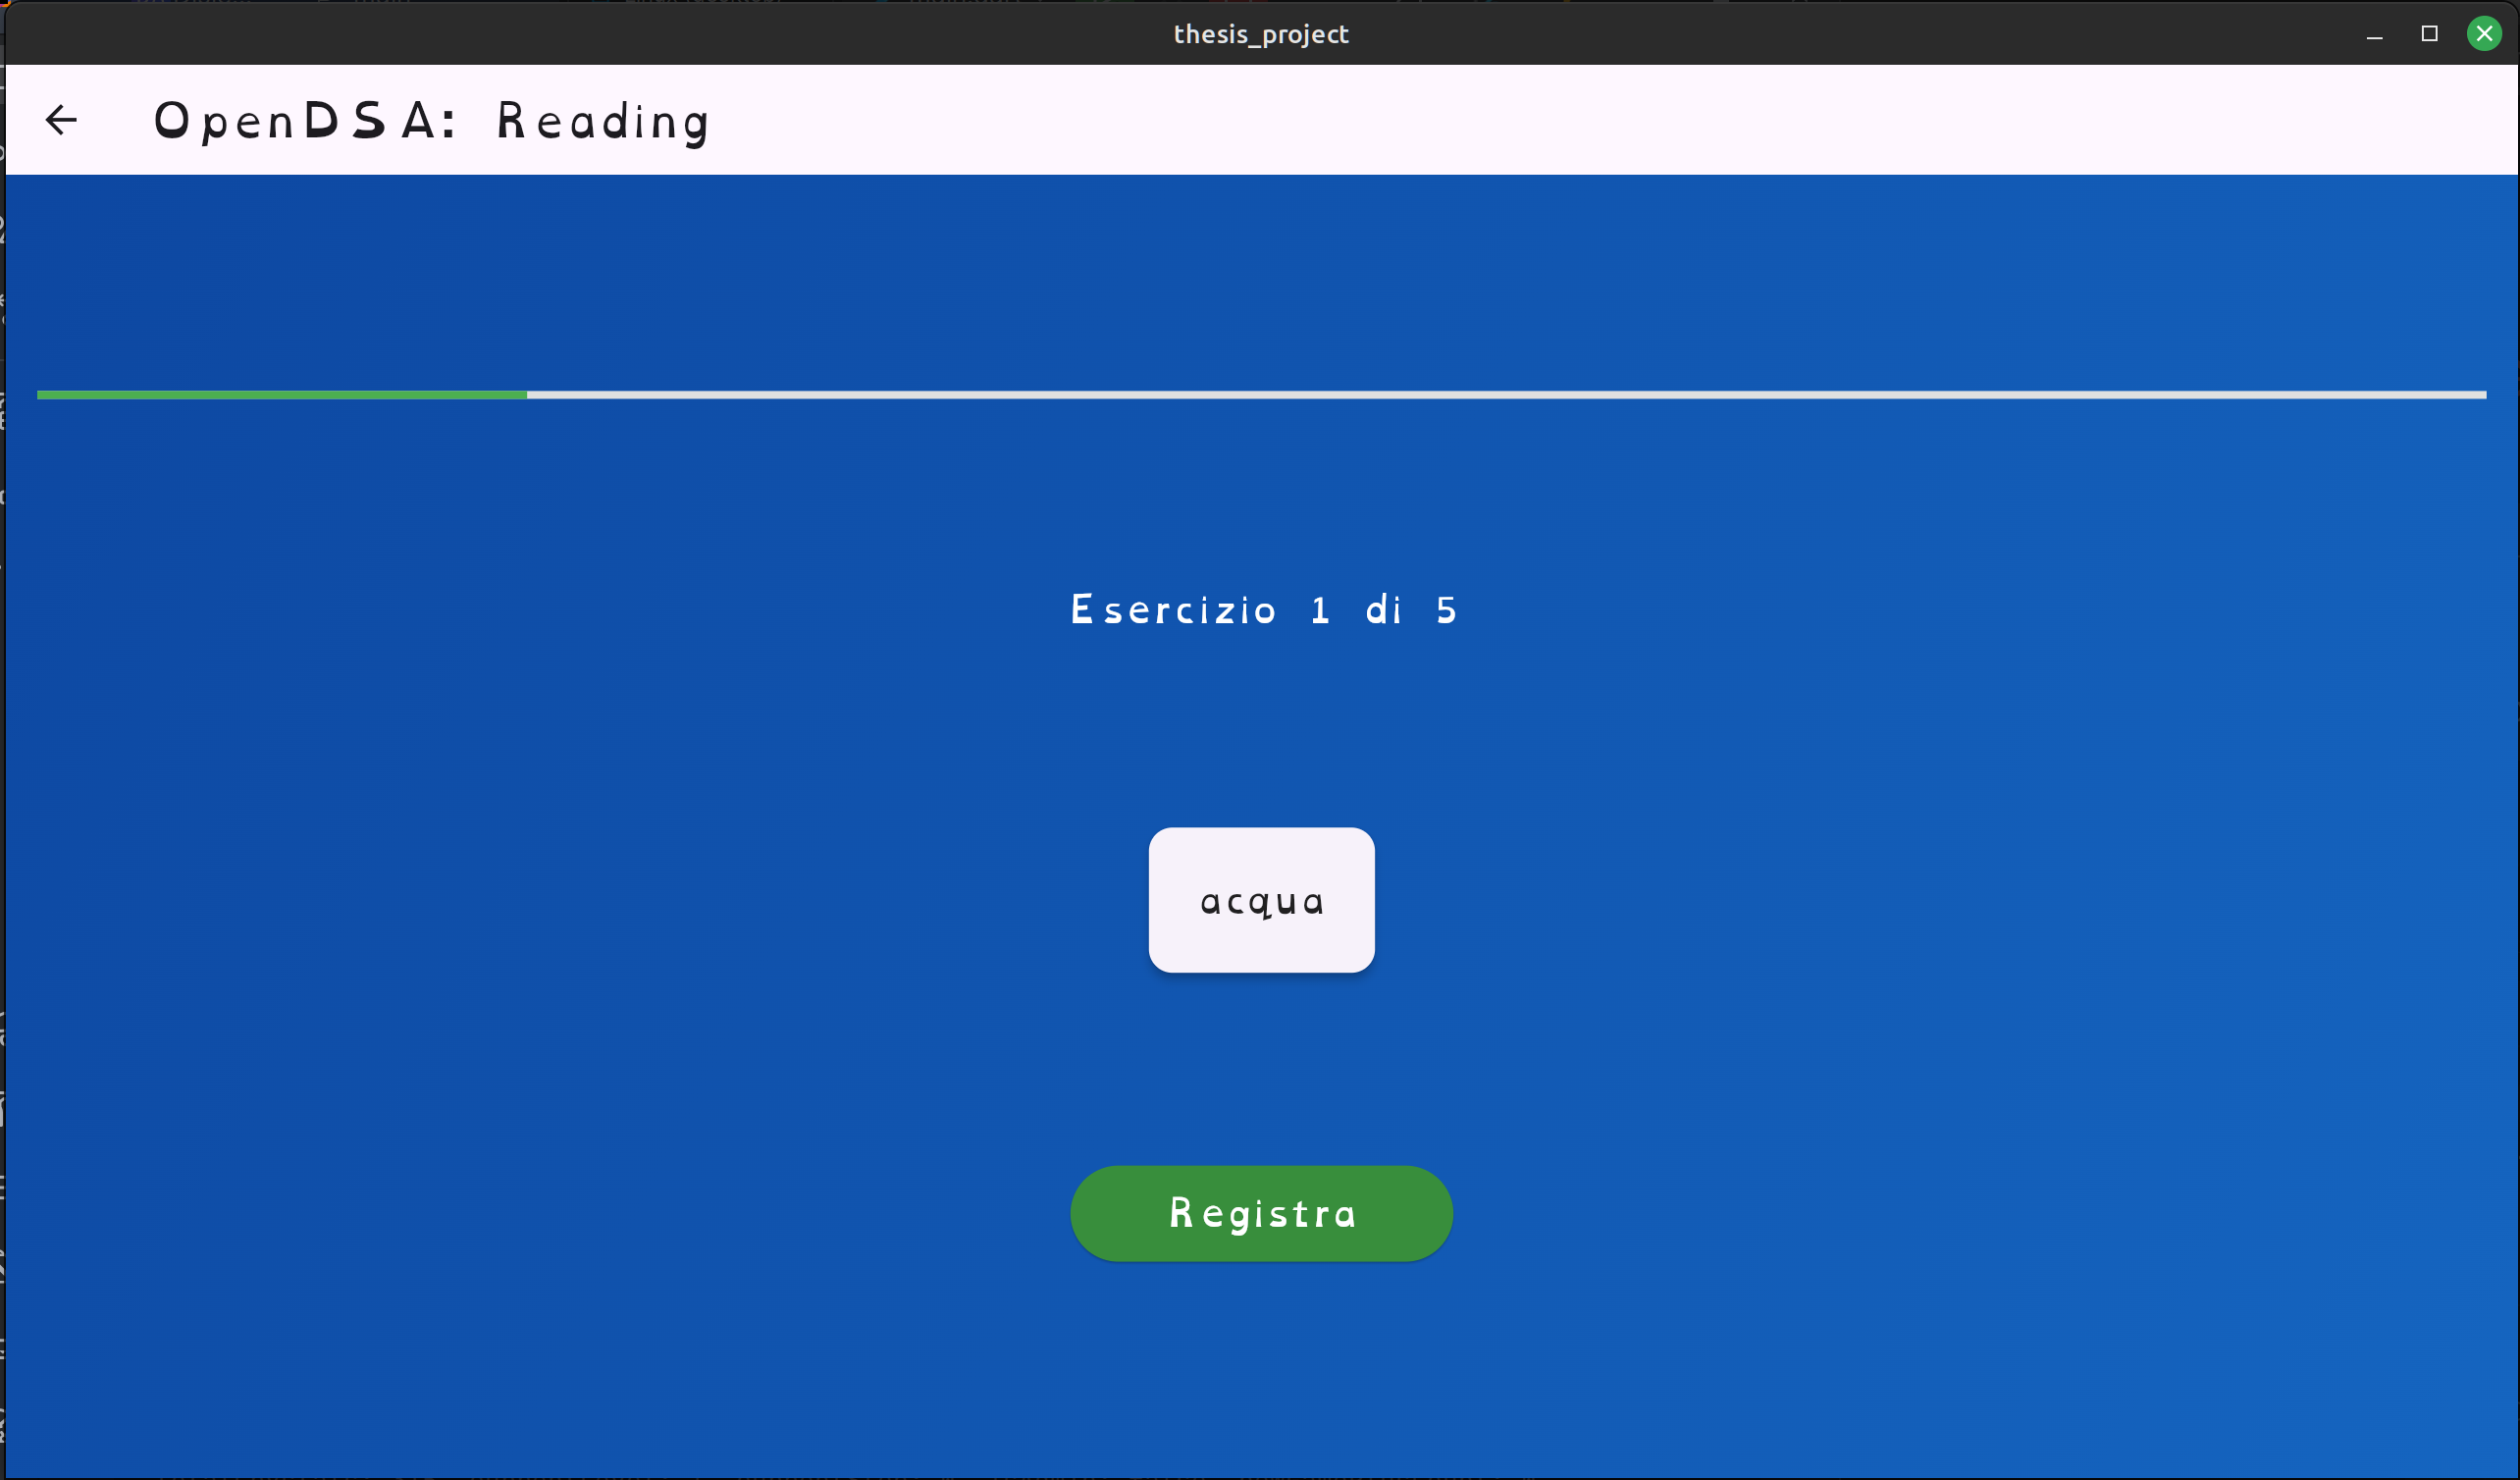
\includegraphics[width=16cm]{Images/6.png}\\
Attraverso il pulsante \textit{"Esercizio di Lettura"} invece, ci verranno proposti un set di 5 esercizi di fila, che dovremo risolvere registrando un file audio attraverso l'uso del microfono. Questo poi, verrà elaborato attraverso il \textit{VoskService} (Servizio che si appoggia alla AI di VOSK) e attraverso le ottimizzazioni degli errori comuni della dislessia (vedere elenco in Appendice B) e \textit{l'Algoritmo di Riconoscimento della Distanza di Levenshtein}, elaborerà l'audio in testo e fornirà un output riconoscitivo. \\

\textit{Algoritmo di Levenshtein}

La \textit{distanza di Levenshtein}, nota anche come \textit{distanza di edit}, è una misura di similarità tra due stringhe. In altre parole, essa quantifica  il numero minimo di operazioni elementari richieste per trasformare una stringa nell'altra. Questa metrica è stata introdotta per la prima volta nel 1965 dal ricercatore russo Vladimir Levenshtein. 

Le operazioni che vengono prese in considerazione sono:
\begin{itemize}
  \item \textbf{Cancellazione} di un carattere;
  \item \textbf{Sostituzione} di un carattere con un altro;
  \item \textbf{Inserimento} di un carattere.
\end{itemize}

Ad esempio, per trasformare la stringa \texttt{"bar"} nella stringa 
\texttt{"biro"} sono necessarie due operazioni:
\begin{enumerate}
  \item Sostituzione di \texttt{'a'} con \texttt{'i'}: 
  \texttt{"bar"} $\rightarrow$ \texttt{"bir"}
  \item Inserimento del carattere \texttt{'o'}: 
  \texttt{"bir"} $\rightarrow$ \texttt{"biro"}
\end{enumerate}
Quindi, la distanza di Levenshtein tra \texttt{"bar"} e \texttt{"biro"} è pari a $2$.

\subsection{Uso e applicazioni}
La distanza di Levenshtein trova impiego in molteplici ambiti:
\begin{itemize}
  \item \textbf{Correttori ortografici}: per suggerire parole candidate 
        quando l'utente commette un errore di digitazione;
  \item \textbf{Riconoscimento OCR e vocale}: per confrontare stringhe 
        di riconoscimento con voci di un dizionario;
  \item \textbf{Analisi di similarità in Data Mining}: per raggruppare 
        o indicizzare stringhe simili;
  \item \textbf{Ricerca di pattern approssimata}: utile quando si cercano 
        corrispondenze imprecise (ad es. motori di ricerca di nomi o keyword);
  \item \textbf{Comparazione di sequenze biologiche}: sebbene spesso si 
        adottino varianti più complesse, la distanza di Levenshtein può 
        costituire un punto di partenza per il confronto di brevi sequenze 
        di DNA o proteine.
\end{itemize}

\subsection{Proprietà e varianti}
Oltre alla definizione classica, esistono varianti dell'algoritmo di Levenshtein 
che tengono conto di altre operazioni, come ad esempio lo \emph{scambio di due 
caratteri adiacenti} (la cosiddetta \emph{distanza di Damerau–Levenshtein}). 
Tuttavia, la forma originaria rimane fra le più utilizzate per semplicità ed 
efficienza computazionale.

\subsection{Formalizzazione della distanza}
La distanza di Levenshtein tra due stringhe $A$ e $B$ è definita come il 
\emph{numero minimo} di operazioni elementari (inserimenti, cancellazioni 
o sostituzioni di un singolo carattere) per convertire la stringa $A$ 
nella stringa $B$. 

\subsubsection{Esempi}
\begin{itemize}
  \item Distanza tra \texttt{"casa"} e \texttt{"cassa"}: 
    \begin{itemize}
      \item \texttt{"casa"} $\rightarrow$ \texttt{"cassa"} (inserimento di \texttt{'s'}),
    \end{itemize}
    quindi distanza $=1$.
  \item Distanza tra \texttt{"gatto"} e \texttt{"matto"}:
    \begin{itemize}
      \item \texttt{"gatto"} $\rightarrow$ \texttt{"matto"} 
            (sostituzione di \texttt{'g'} con \texttt{'m'}),
    \end{itemize}
    quindi distanza $=1$.
  \item Distanza tra \texttt{"sarto"} e \texttt{"sorto"}:
    \begin{itemize}
      \item \texttt{"sarto"} $\rightarrow$ \texttt{"sorto"} 
            (sostituzione di \texttt{'a'} con \texttt{'o'}),
    \end{itemize}
    quindi distanza $=1$.
\end{itemize}
Naturalmente, esempi più complessi richiederanno un numero maggiore di passi.

\subsection{Descrizione dell'algoritmo}
Un metodo classico per calcolare la distanza di Levenshtein tra due stringhe 
\texttt{str1} e \texttt{str2} di lunghezze \texttt{lenStr1} e \texttt{lenStr2}, 
rispettivamente, si basa sulla costruzione di una matrice bidimensionale 
di dimensione $(\texttt{lenStr1} + 1) \times (\texttt{lenStr2} + 1)$.

\begin{itemize}
  \item \textbf{Dimensione della matrice}: la dimensione è $(n + 1) \times (m + 1)$ 
        dove $n = \texttt{lenStr1}$ e $m = \texttt{lenStr2}$;
  \item \textbf{Interpretazione}: ogni cella $d[i,j]$ della matrice rappresenta 
        la distanza di Levenshtein tra i primi $i$ caratteri di \texttt{str1} 
        e i primi $j$ caratteri di \texttt{str2}.
\end{itemize}

L'algoritmo si basa su un approccio \emph{dinamico}:

\begin{enumerate}
  \item Inizializzazione: le prime righe e le prime colonne della matrice 
        vengono valorizzate con indici crescenti (i costi necessari per 
        trasformare una stringa di lunghezza $i$ in una stringa vuota o viceversa);
  \item Ricorrenza: per ogni coppia di indici $(i,j)$ si controlla se i caratteri 
        corrispondenti delle due stringhe sono uguali. In caso positivo, si 
        aggiorna la cella $d[i,j]$ con il valore di $d[i-1,j-1]$. In caso negativo, 
        si calcola la minima distanza tra l’operazione di \textit{cancellazione}, 
        \textit{inserimento} o \textit{sostituzione} e si somma 1 come costo 
        dell’operazione.
\end{enumerate}

Lo pseudocodice di riferimento è il seguente:

\begin{lstlisting}[caption=Pseudocodice dell'algoritmo di Levenshtein, label=lst:levenshtein]
int LevenshteinDistance(char str1[1..lenStr1], char str2[1..lenStr2])
   // d[i1, i2] conterra' la distanza di Levenshtein tra
   // i primi i1 caratteri di str1 e i primi i2 caratteri di str2.
   declare int d[0..lenStr1, 0..lenStr2]
   declare int i1, i2, cost

   for i1 from 0 to lenStr1
       d[i1, 0] := i1
   for i2 from 0 to lenStr2
       d[0, i2] := i2

   for i1 from 1 to lenStr1
       for i2 from 1 to lenStr2
           if str1[i1 - 1] = str2[i2 - 1] then
               cost := 0
               d[i1, i2] := d[i1 - 1, i2 - 1]
           else
               cost := 1
               d[i1, i2] := minimum(
                   d[i1 - 1, i2] + 1,       // cancellazione
                   d[i1, i2 - 1] + 1,       // inserimento
                   d[i1 - 1, i2 - 1] + cost // sostituzione
               )

   return d[lenStr1, lenStr2]
\end{lstlisting}

\subsection{Esempio di calcolo dettagliato}
Si consideri il confronto fra \texttt{"cane"} e \texttt{"gatto"}:

\begin{itemize}
  \item $\texttt{"cane"} \rightarrow \texttt{"gane"}$ (sostituzione di \texttt{'c'} con \texttt{'g'});
  \item $\texttt{"gane"} \rightarrow \texttt{"gatne"}$ (inserimento di \texttt{'t'} prima di \texttt{'n'});
  \item $\texttt{"gatne"} \rightarrow \texttt{"gatto"}$ (sostituzione di \texttt{'n'} con \texttt{'t'}).
\end{itemize}
In questo caso la distanza calcolata è $3$. 

\subsection{Analisi dell'algoritmo}
\textbf{Complessità}
La complessità temporale dell'algoritmo classico è $O(n \cdot m)$, dove:
\begin{itemize}
  \item $n = \texttt{lenStr1}$
  \item $m = \texttt{lenStr2}$
\end{itemize}
La complessità in memoria è anch'essa $O(n \cdot m)$, essendo necessaria la 
costruzione di una matrice di dimensioni $(n+1) \times (m+1)$.

\textbf{Ottimizzazioni}
Sono possibili varie ottimizzazioni, tra cui:
\begin{itemize}
  \item \textbf{Spazio}: esistono versioni che riducono l’utilizzo di memoria 
        salvando solo la riga corrente e la riga precedente della matrice 
        (o di colonna in colonna), abbassando la complessità spaziale a $O(\min(n,m))$.
  \item \textbf{Pruning}: per applicazioni in cui è noto a priori un limite 
        superiore alla distanza massima d’interesse, si possono adottare 
        metodi di \emph{taglio} (pruning) per interrompere l’algoritmo quando 
        viene superata tale soglia.
\end{itemize}

La distanza di Levenshtein rappresenta un riferimento fondamentale nello studio  delle stringhe in vari campi dell’informatica e dell’elaborazione dei dati. Il  suo algoritmo, pur nella semplicità, costituisce un ottimo esempio di utilizzo della programmazione dinamica e fornisce risultati utili in tutte quelle situazioni in cui è importante stimare quanto due stringhe differiscano tra loro.\cite{wikipedia:levenshtein} \\\\

Questo algoritmo viene inglobato all'interno del vosk\_service.dart (classe in Appendice B) assieme al codice fonetico, in modo da garantire che il risultato venga elaborato contestualmente agli errori di pronuncia classici che possono essere commessi (per pronuncia, dialetto o influenza regionale). Di seguito le funzioni che si occupa di questo passaggio:\\\\

\begin{lstlisting} [caption=Calcolo della Similarita' Fonetica, label=lst:Similarita' Fonetica]
  // Mappa per errori comuni (usata nelle funzioni di similarita')
  static const Map<String, List<String>> _commonDyslexicConfusions = {
    'b': ['d', 'p'],
    'd': ['b', 'q'],
    'p': ['q', 'b'],
    'q': ['p', 'd'],
    'm': ['n', 'w'],
    'n': ['m'],
    'a': ['e'],
    'e': ['a'],
    's': ['z'],
    'z': ['s'],
    'f': ['v'],
    'v': ['f'],
  };

double _calculatePhoneticSimilarity(String s1, String s2) {
    String phonetic1 = _getPhoneticCode(s1);
    String phonetic2 = _getPhoneticCode(s2);
    return _calculateLevenshteinSimilarity(phonetic1, phonetic2);
  }

  String _getPhoneticCode(String text) {
    var result = text.toLowerCase();
    final Map<String, String> phoneticRules = {
      'chi': 'ki',
      'che': 'ke',
      'ghi': 'gi',
      'ghe': 'ge',
      'gn': 'ñ',
      'gl': 'ʎ',
      'sc': 'ʃ',
      'qu': 'k',
      'gu': 'g',
      'z': 'ts',
      'zz': 'ts',
    };
    for (var entry in phoneticRules.entries) {
      result = result.replaceAll(entry.key, entry.value);
    }
    result = result.replaceAll(RegExp(r'([aeiou])\1+'), r'$1');
    return result;
  }
  
    double _calculateTextSimilarity(String text1, String text2) {
    if (text1 == text2) return 1.0;
    if (text1.isEmpty || text2.isEmpty) return 0.0;
    const double levenshteinWeight = 0.4;
    const double phoneticWeight = 0.3;
    const double confusionWeight = 0.3;
    double levenshteinScore = _calculateLevenshteinSimilarity(text1, text2);
    double phoneticScore = _calculatePhoneticSimilarity(text1, text2);
    double confusionScore = _calculateConfusionSimilarity(text1, text2);
    return (levenshteinScore * levenshteinWeight) +
        (phoneticScore * phoneticWeight) +
        (confusionScore * confusionWeight);
  }

  double _calculateConfusionSimilarity(String s1, String s2) {
    if (s1.length != s2.length) return 0.0;
    int matchCount = 0;
    for (int i = 0; i < s1.length; i++) {
      if (s1[i] == s2[i]) {
        matchCount++;
        continue;
      }
      if (_commonDyslexicConfusions.containsKey(s1[i]) &&
          _commonDyslexicConfusions[s1[i]]!.contains(s2[i])) {
        matchCount++;
      }
    }
    return matchCount / s1.length;
  }
\end{lstlisting}
Questo ha permesso una maggiore facilità per il Modello di IA nell'interpretare correttamente quelle parole difficili per i bambini che soffrono di dislessia, avendo cura della loro difficoltà e delle eventuali problematiche che possono incorrere nell'utilizzo della App.
\pagebreak

\subsection{Il Feedback dell'Esercizio}
Tornando invece alla User Journey, il passaggio successivo a quello del \textit{Riconoscimento Vocale}, a seguito della produzione ed eliminazione del file audio registrato in formato ".wav" con il plugin \textbf{recorder} è il feedback utente.\\\\
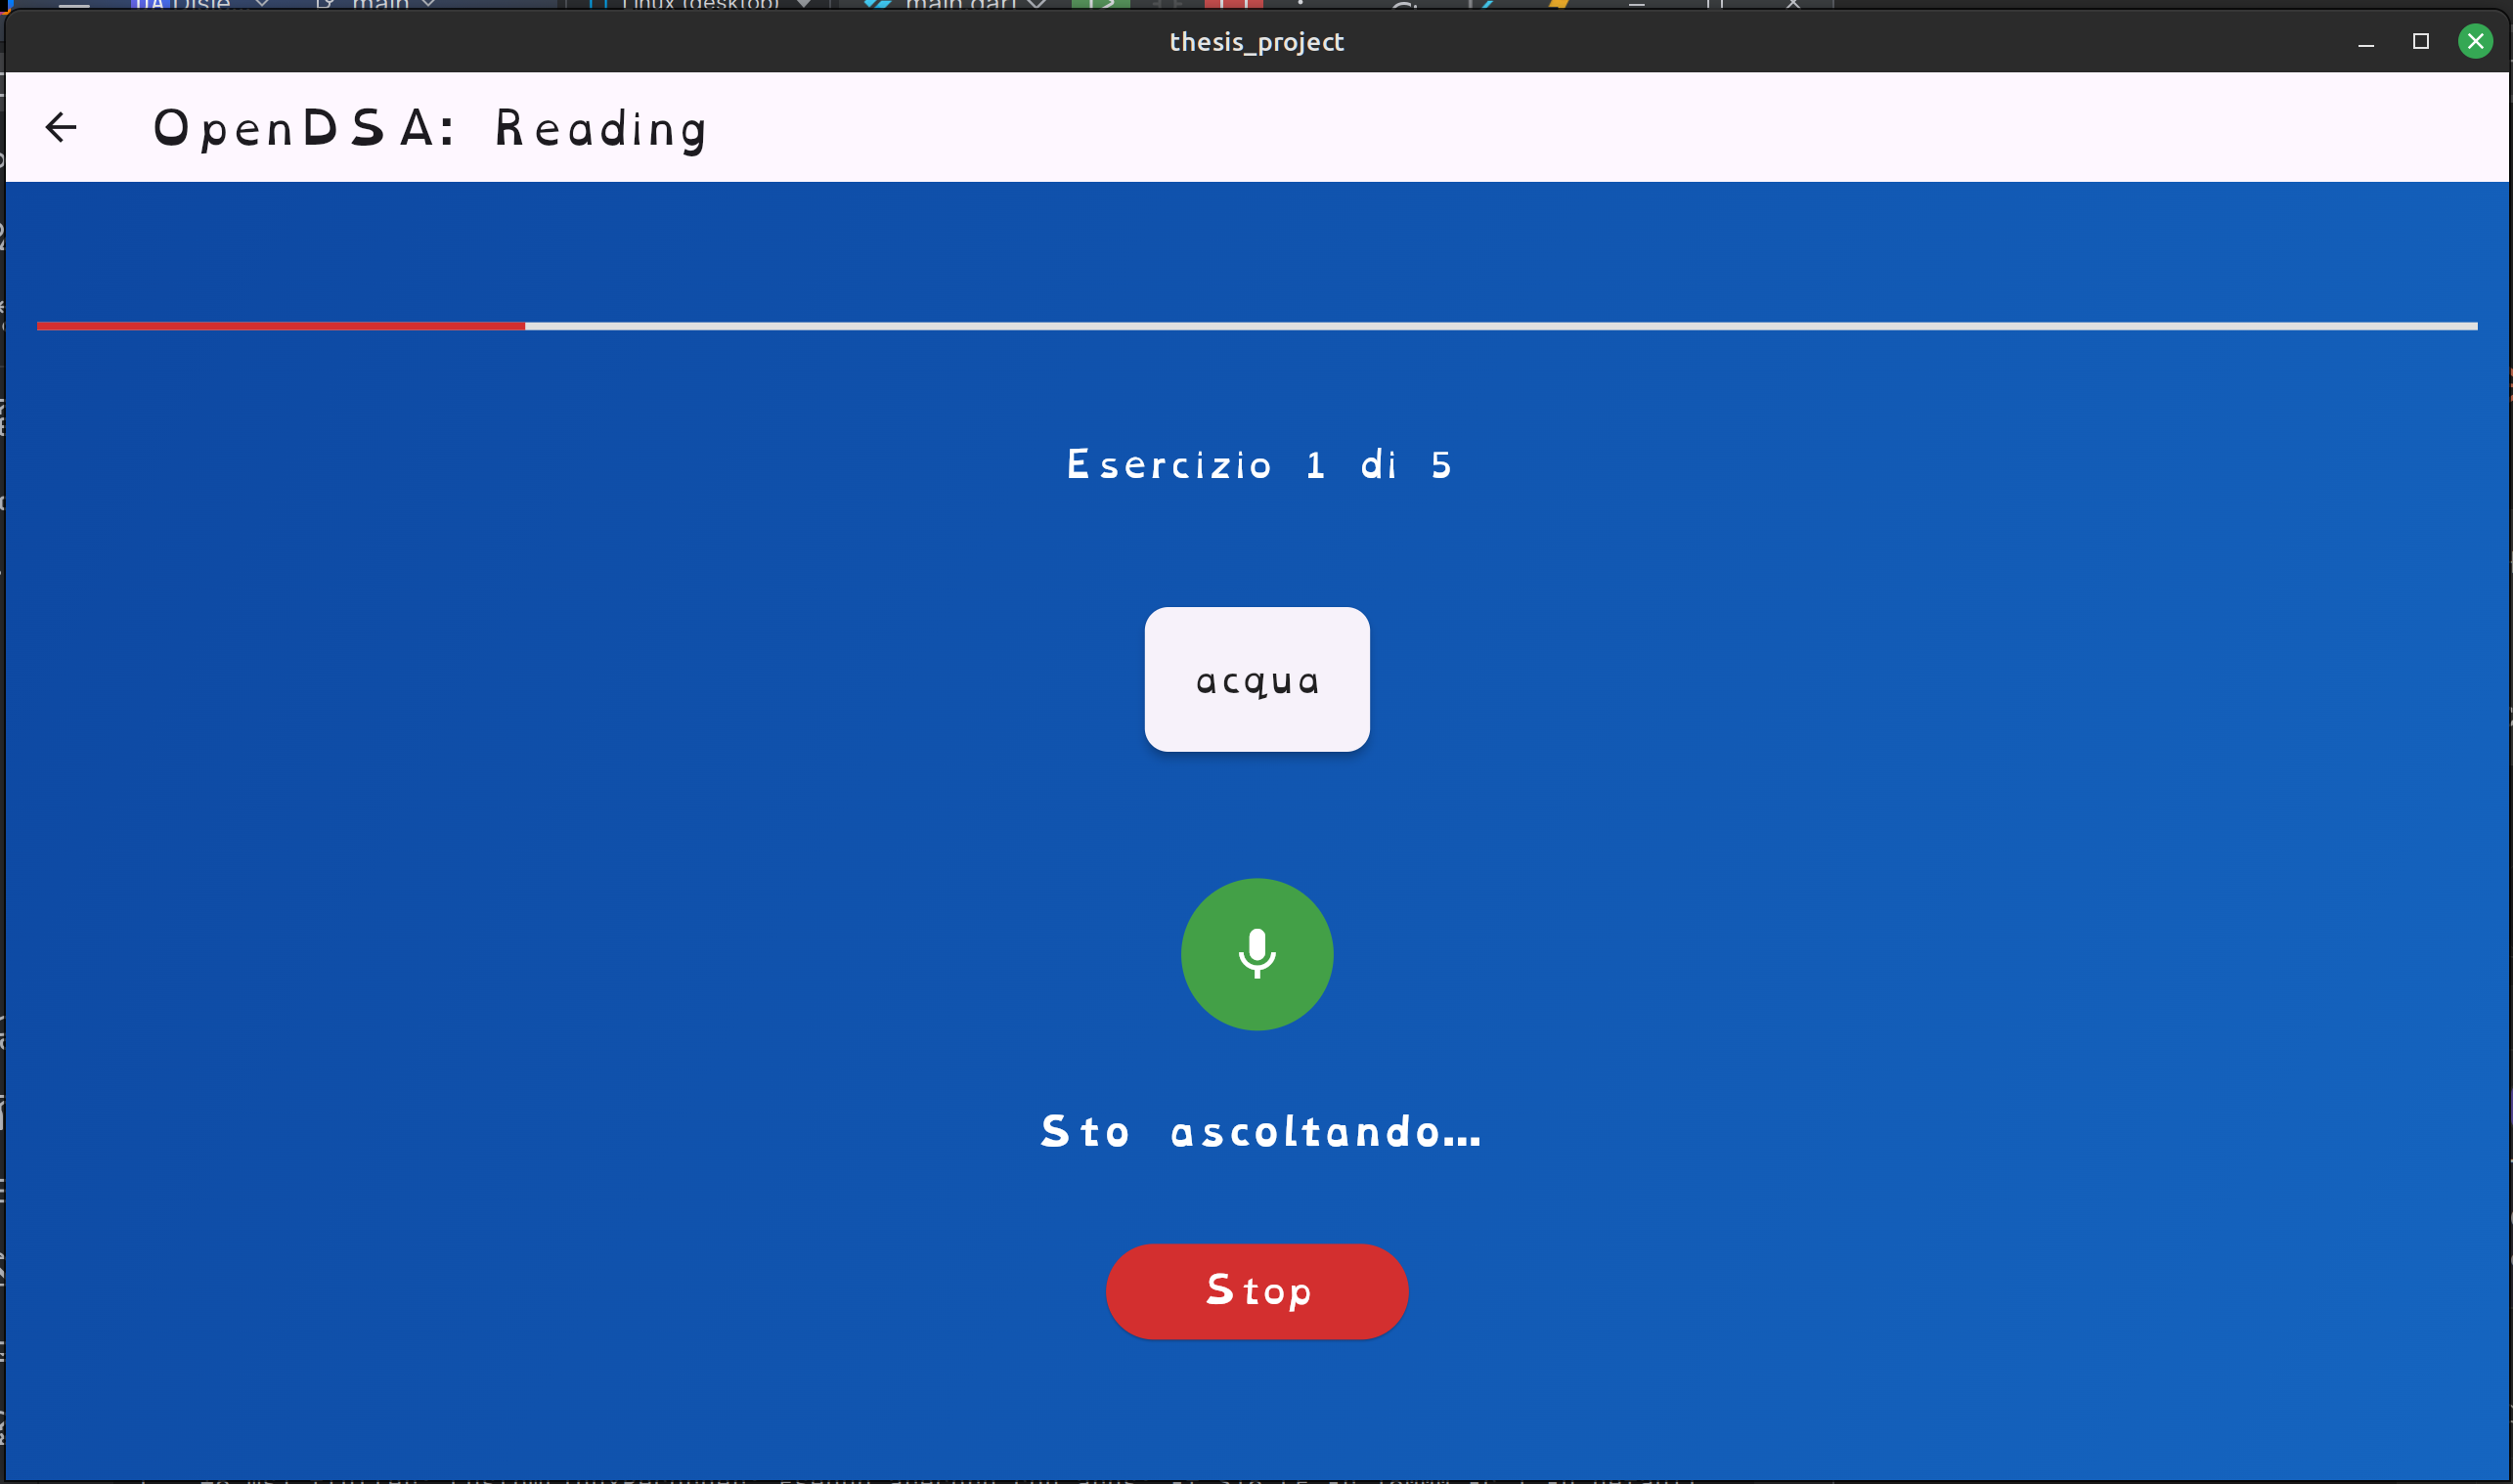
\includegraphics[width=16cm]{Images/7.png}\\
A questo proposito è bene specificare che l'output del feedback visivo è stato sapientemente pensato con colori ed emoji (caricate direttamente dal sistema essendo in codice UNICODE) in modo da dare anche un contesto ben chiaro dell'andamento dell'esercizio (oltre al riepilogo di Cristalli e Accuratezza ottenuti). Per essere ancora più meticolosi, alla fine della serie di 5 esercizi, viene proposto un quadro riepilogativo finale.\\\\
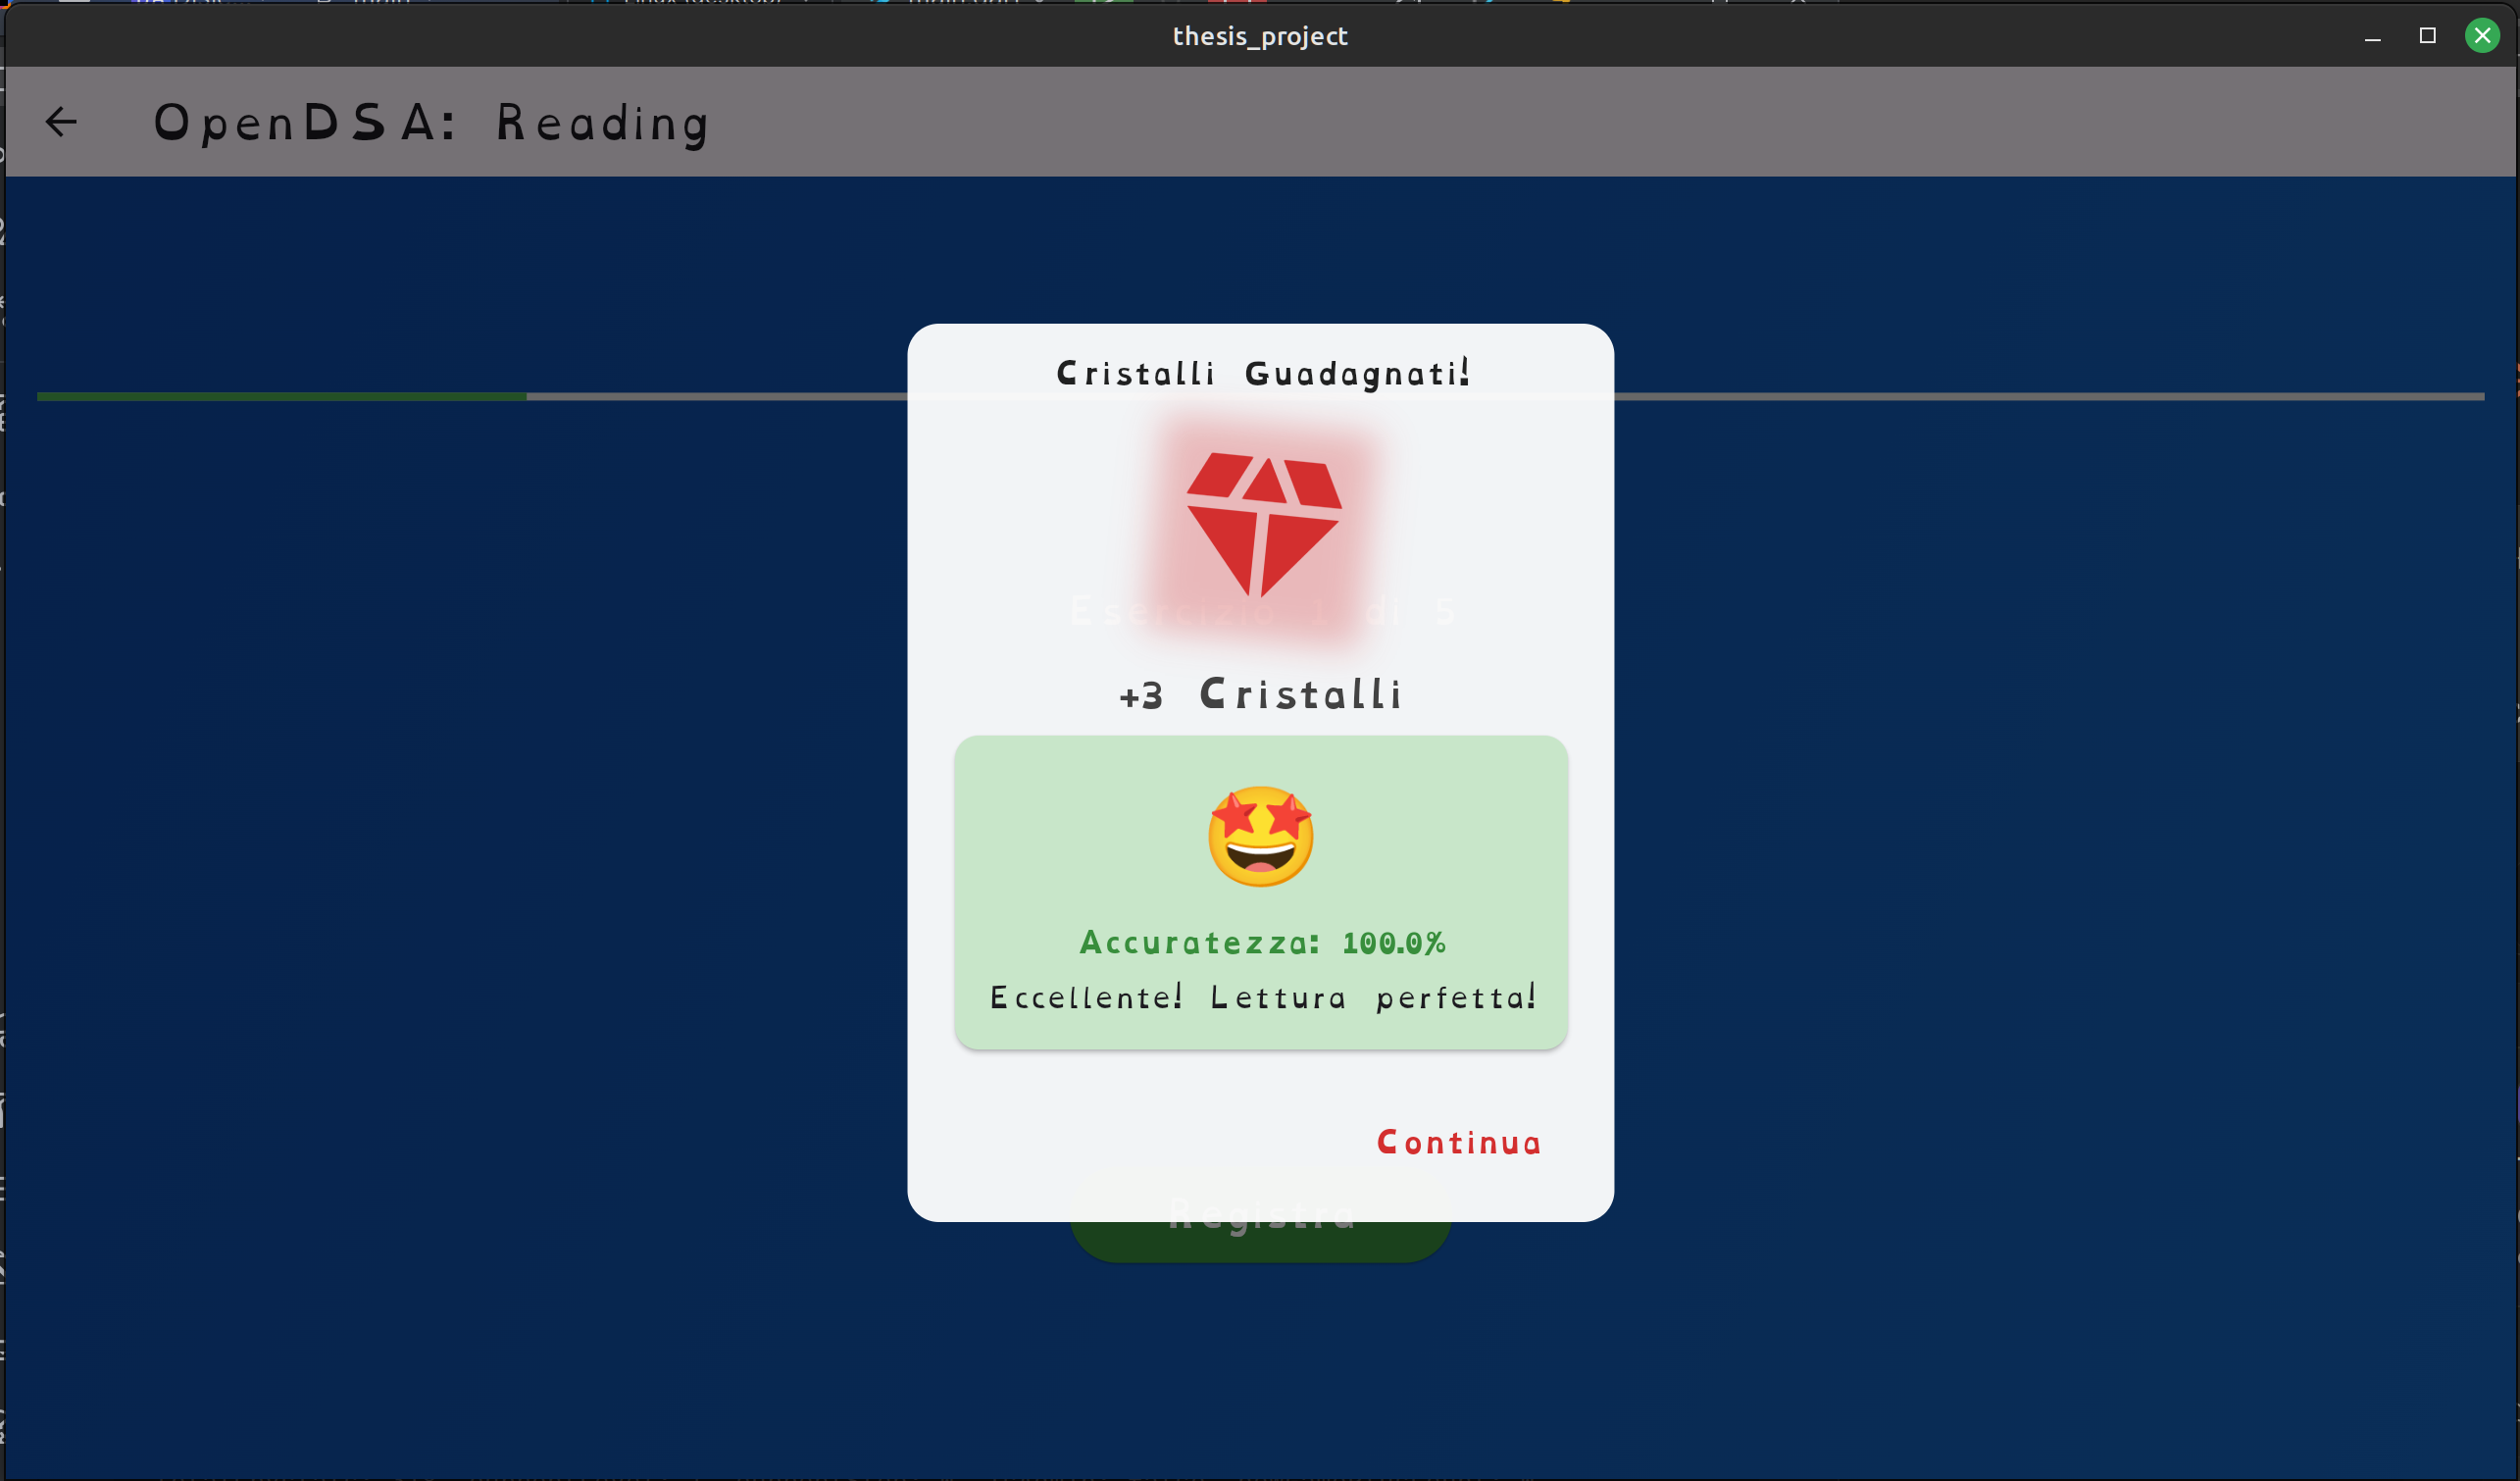
\includegraphics[width=16cm]{Images/8.png}\\
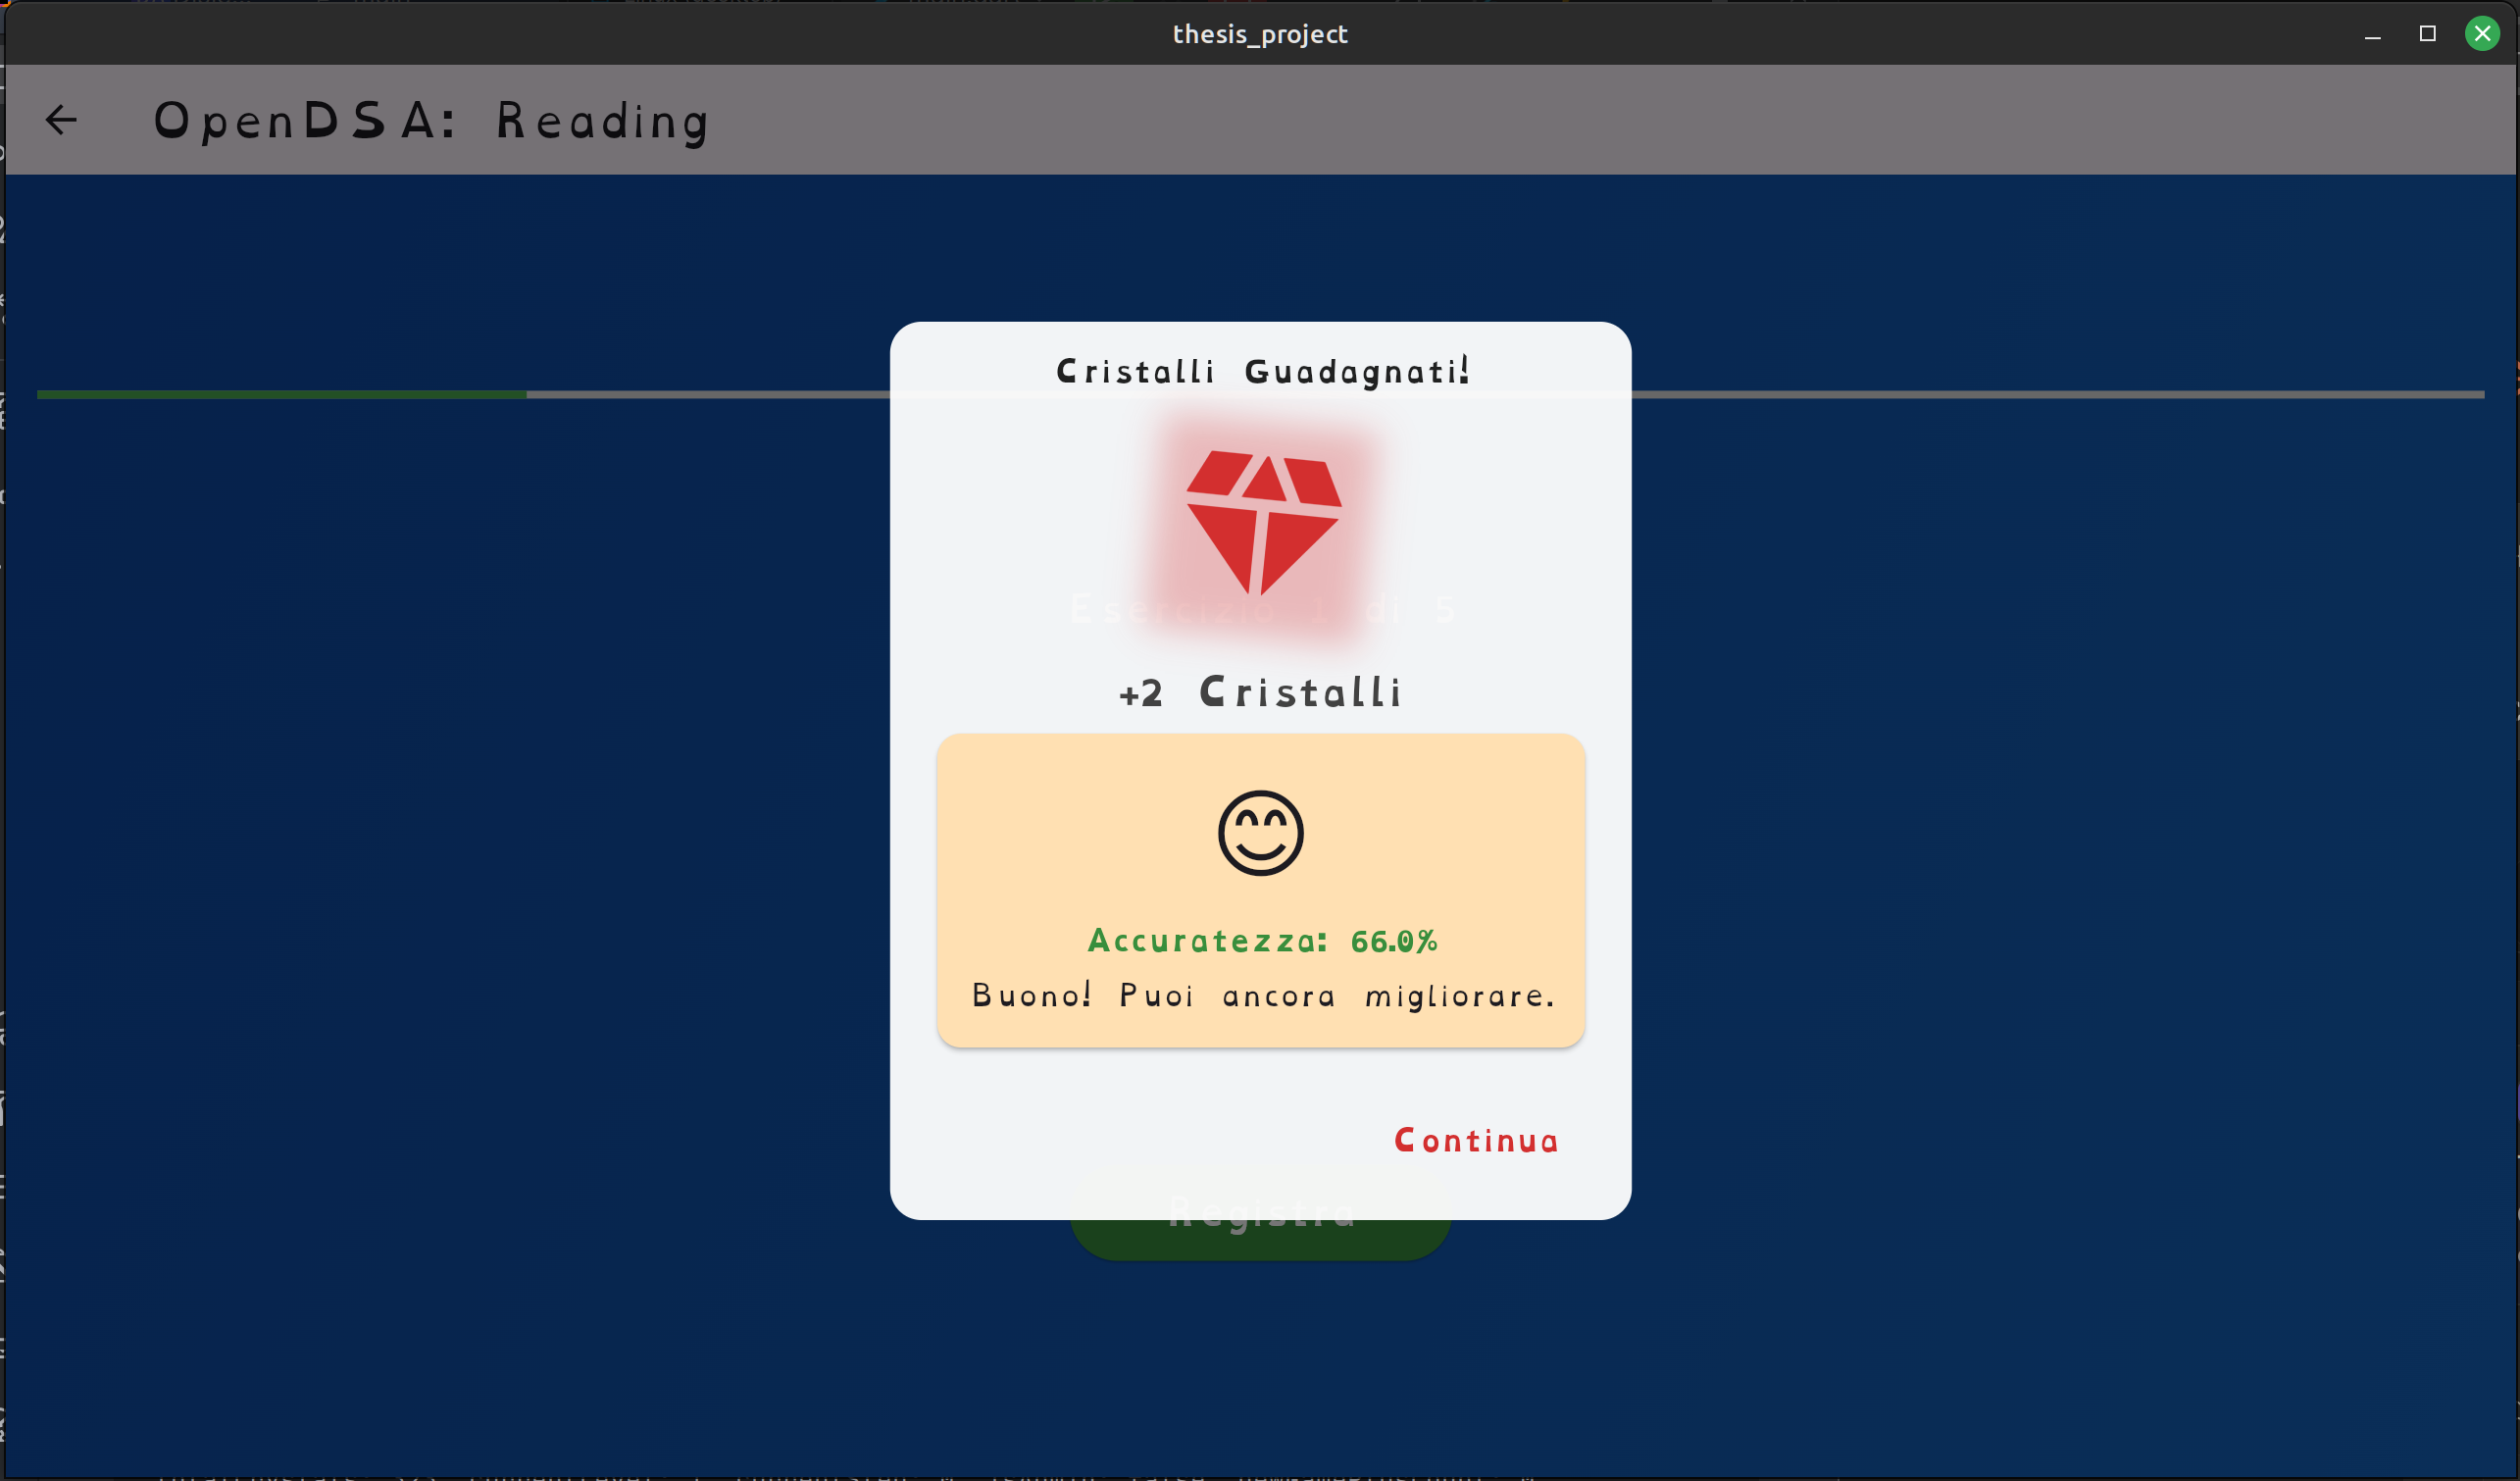
\includegraphics[width=16cm]{Images/9.png}\\
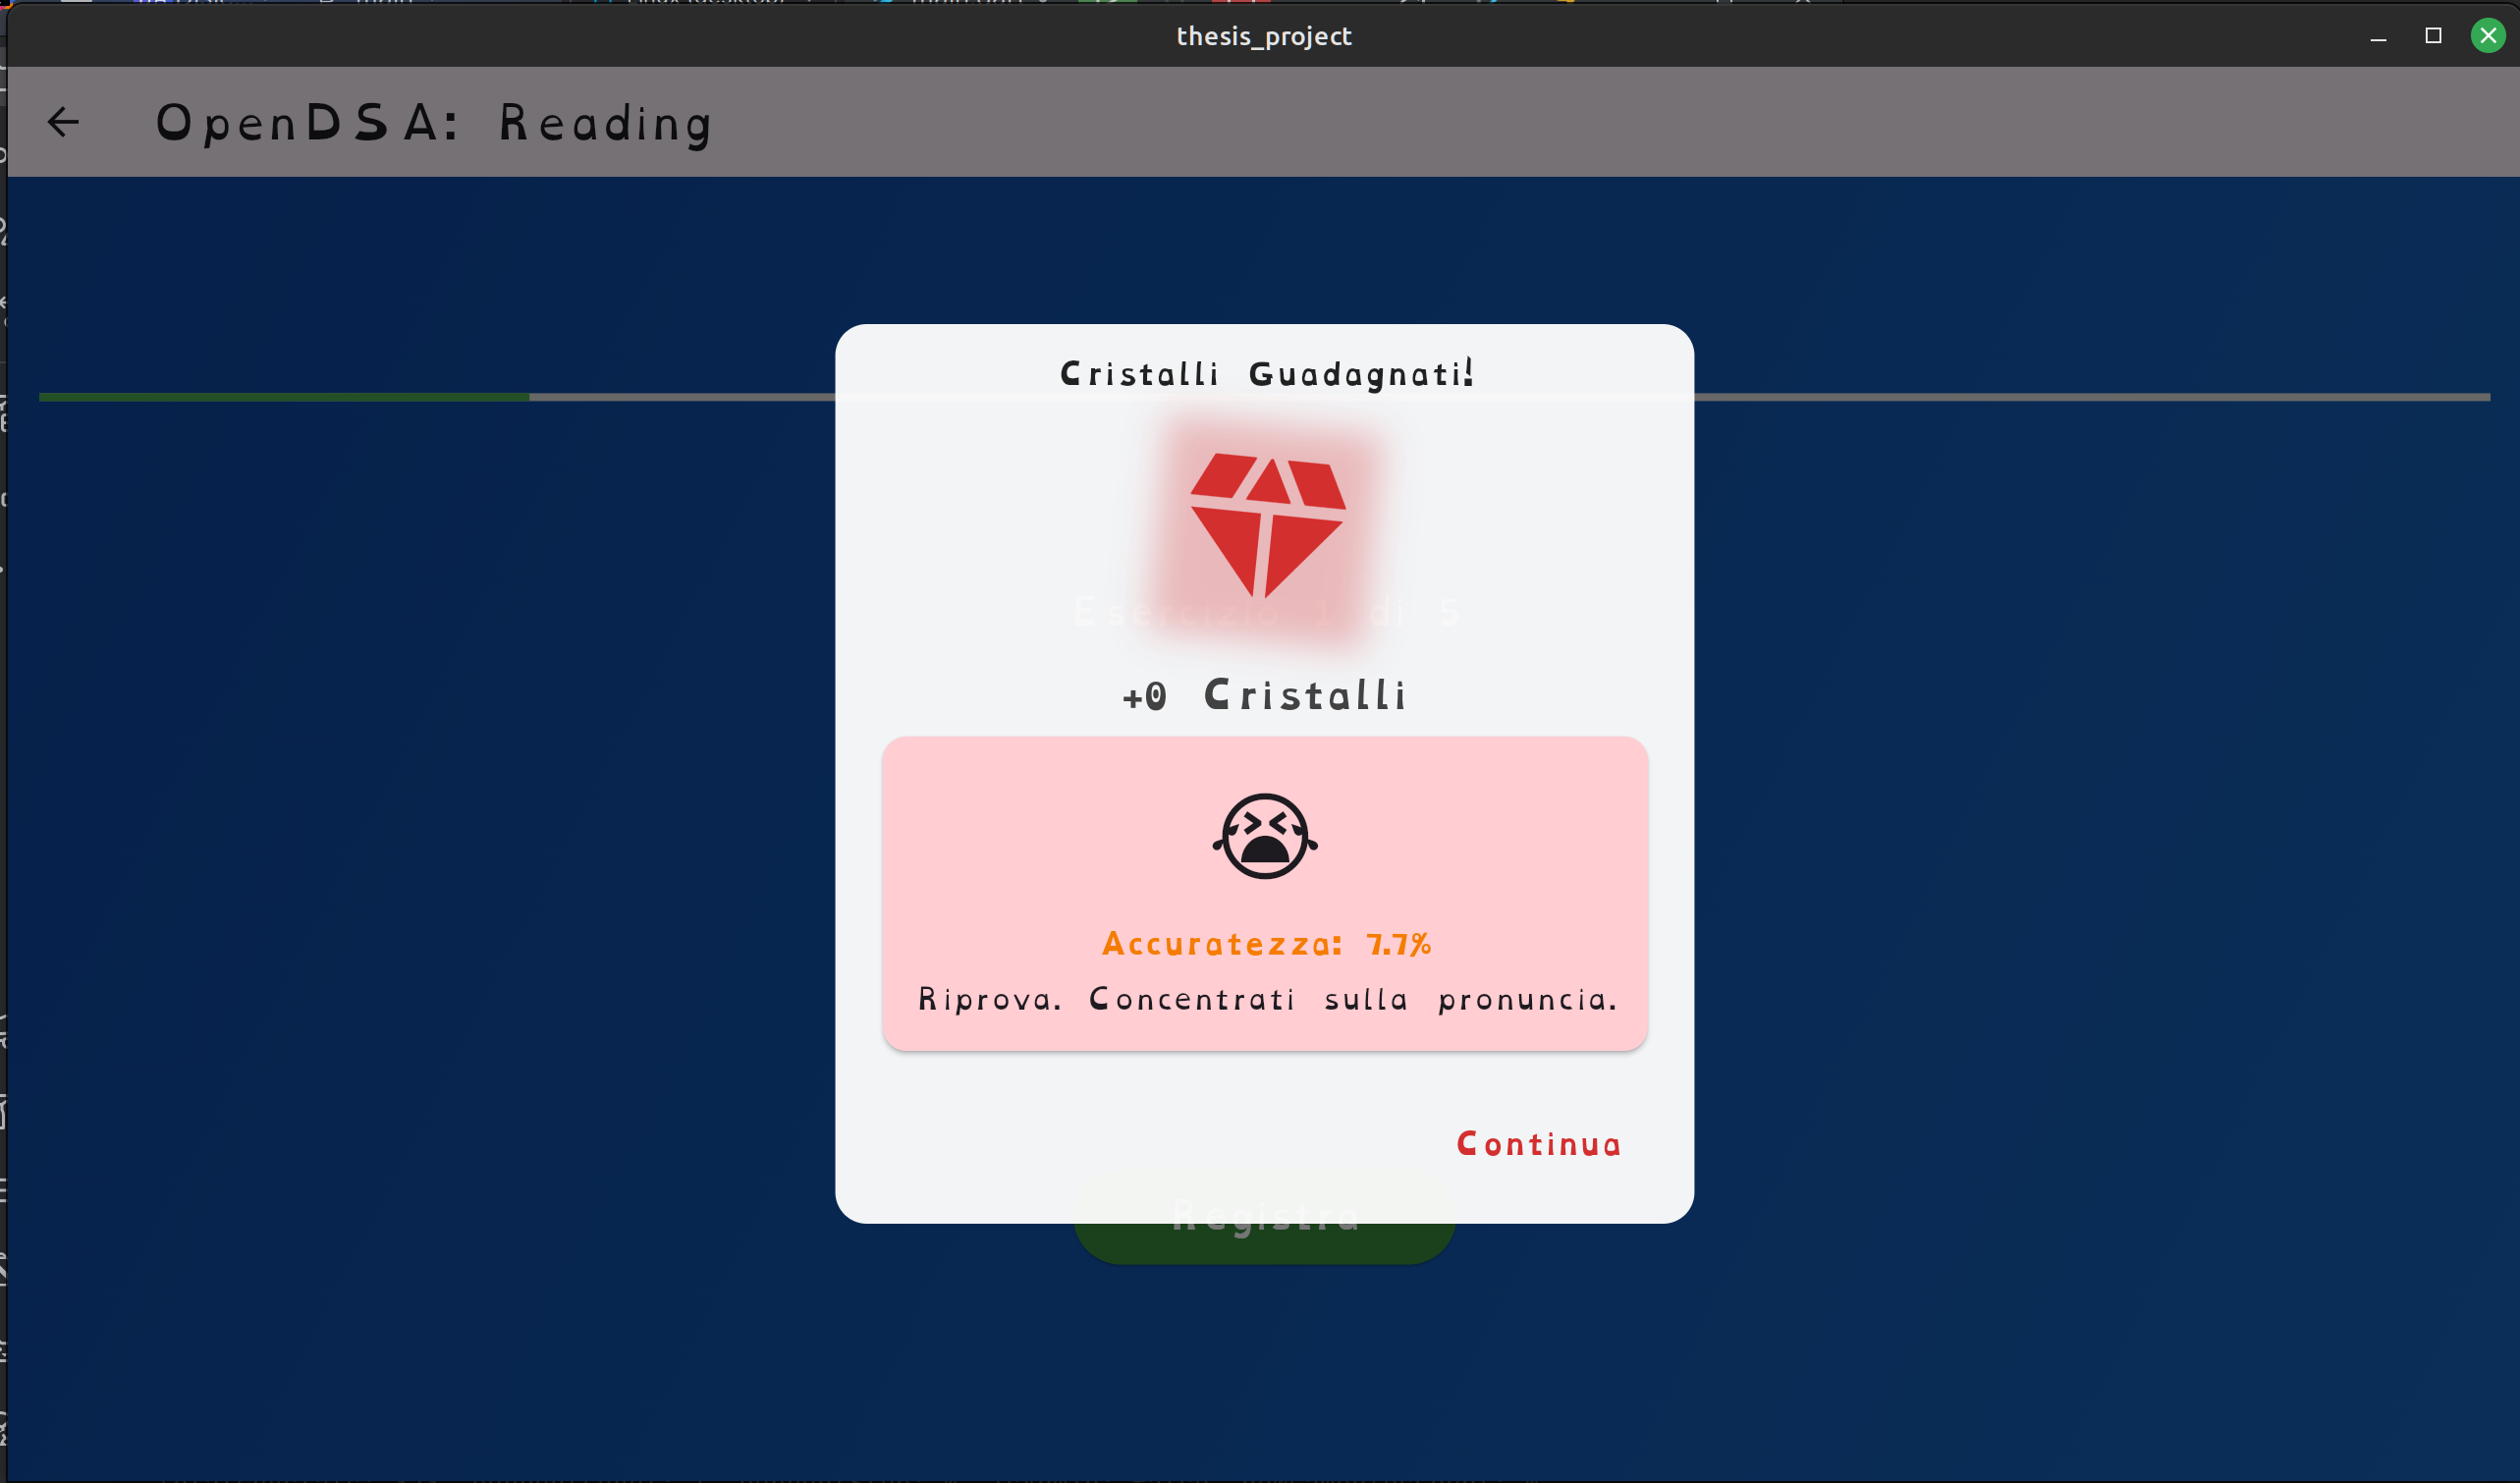
\includegraphics[width=16cm]{Images/10.png}\\

Il \textit{Gioco} a questo punto ci chiederà se vogliamo \textit{Continuare}, con un'altra serie di 5 esercizi, o se vogliamo concludere la nostra sessione di allenamento, tornando di fatto alla schermata principale.\\\\
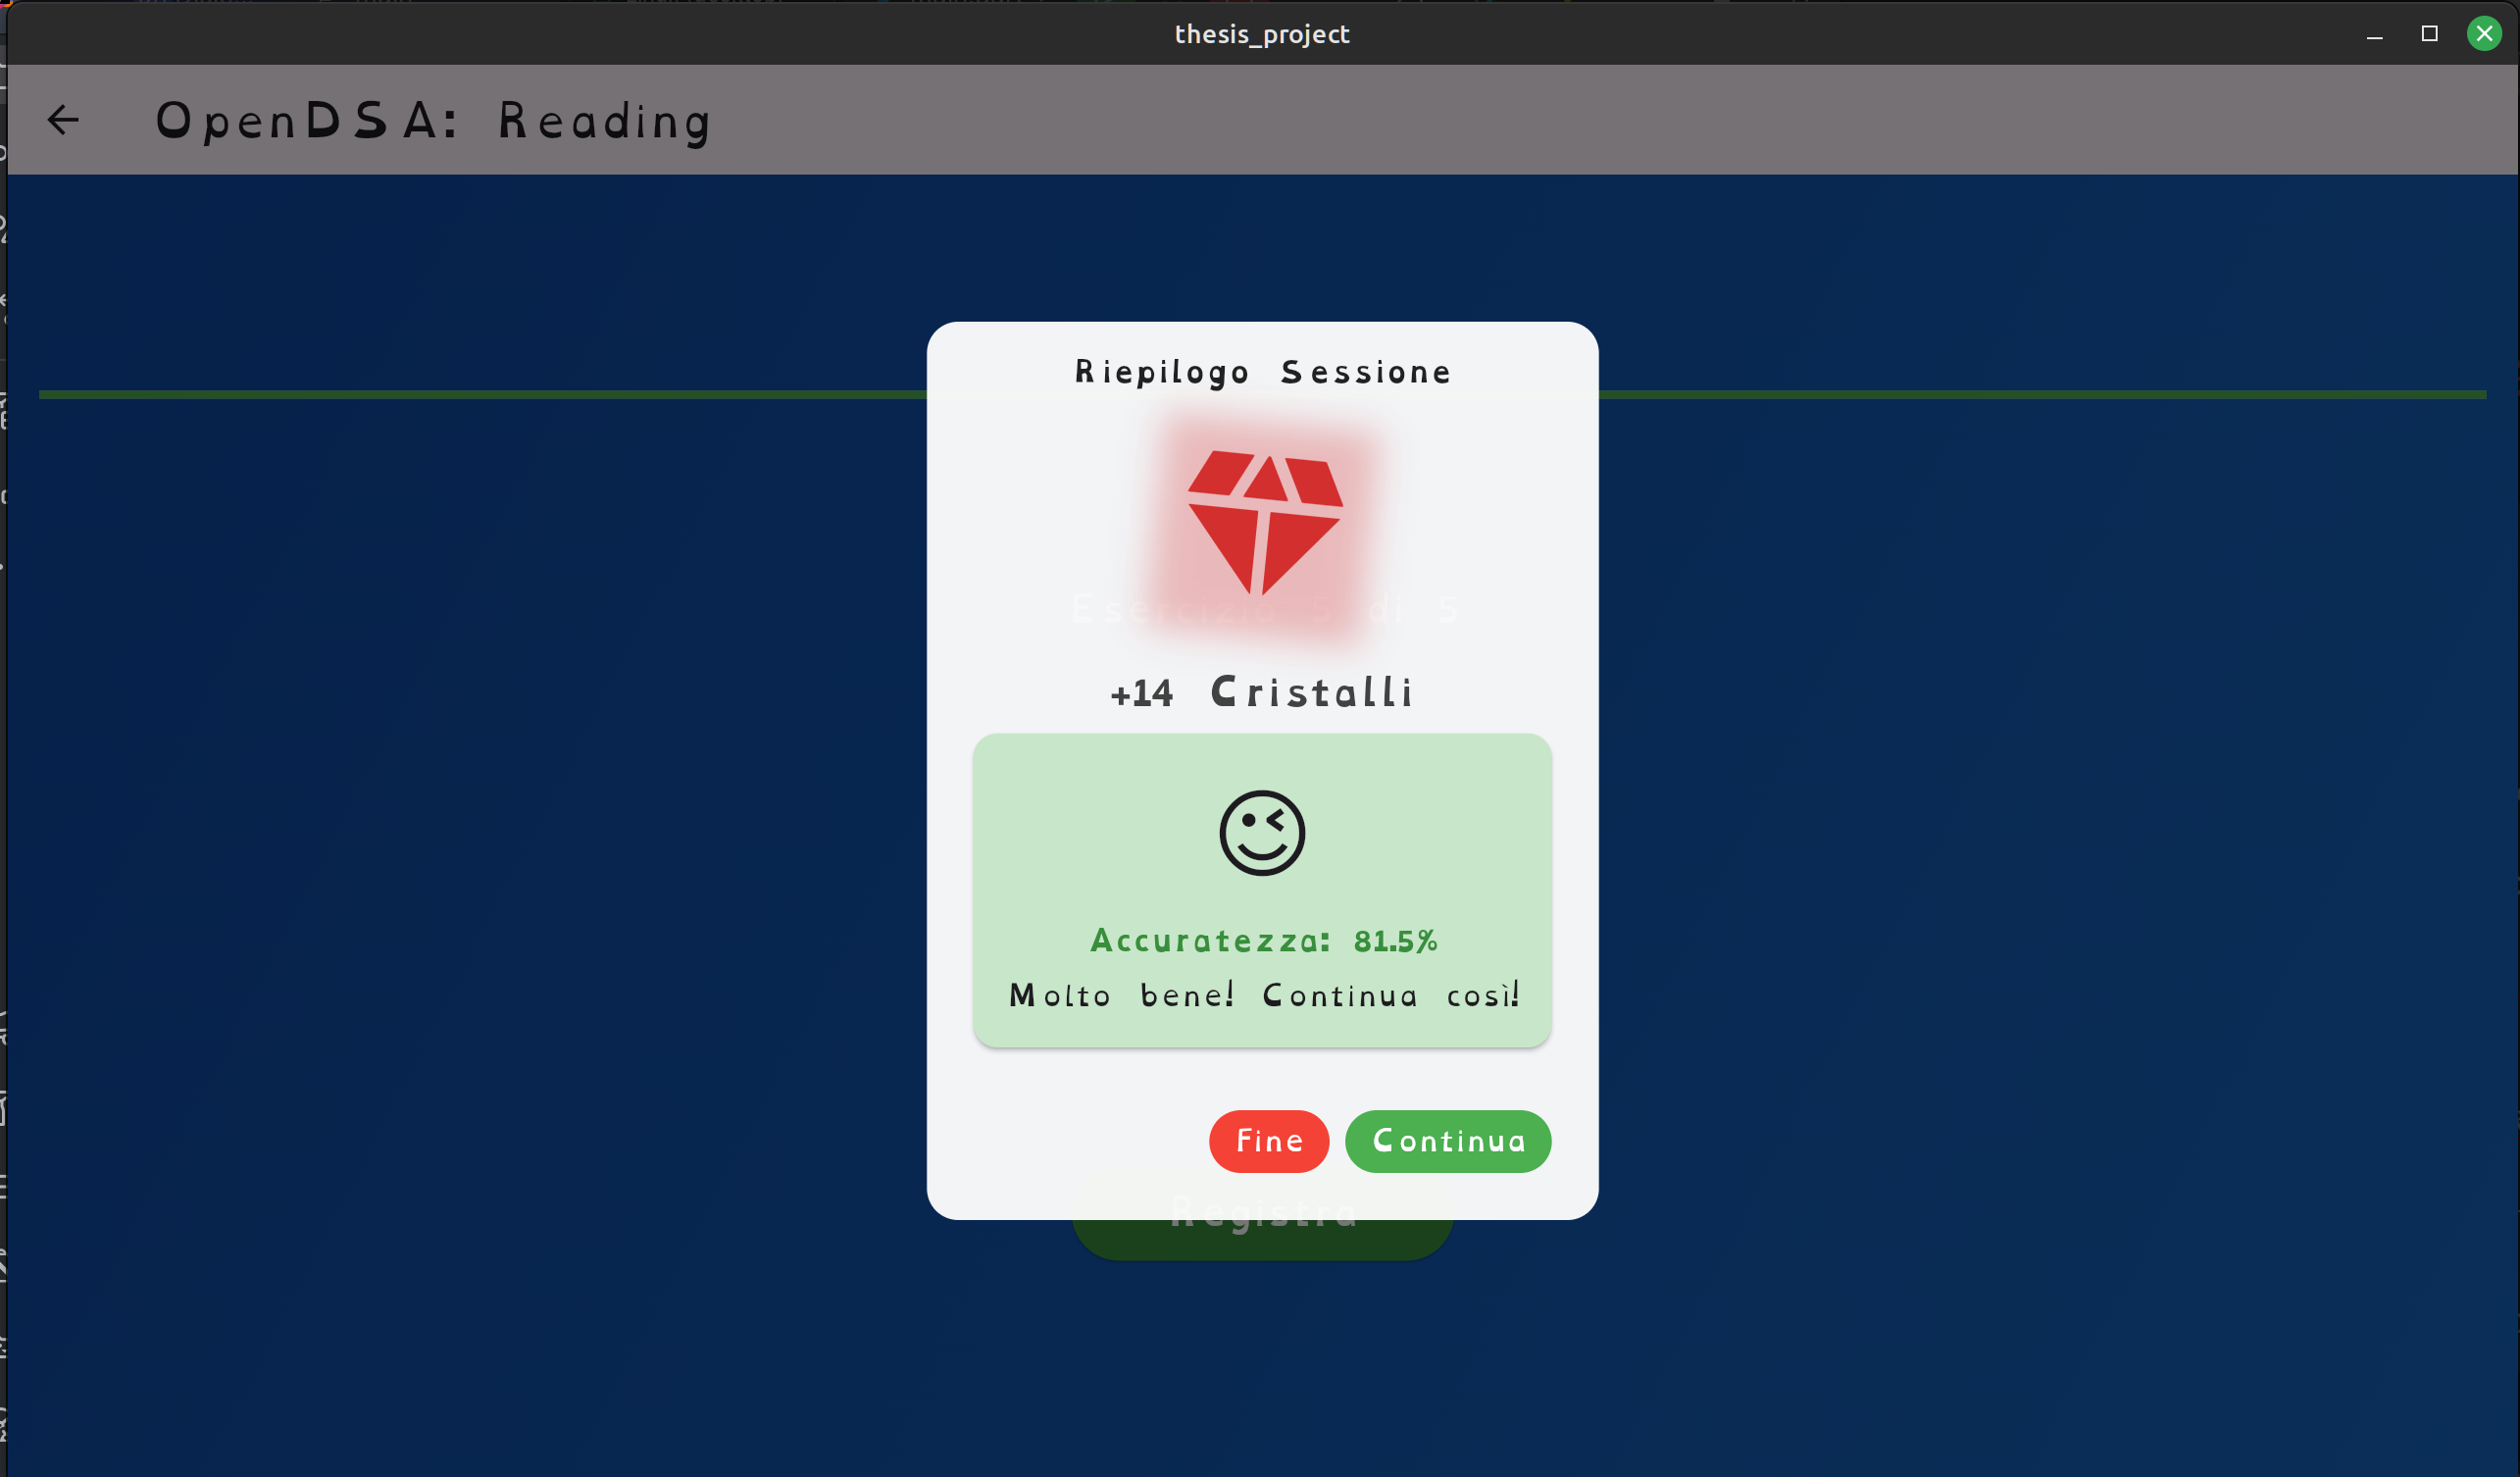
\includegraphics[width=16cm]{Images/11.png}\\
\pagebreak
\section{Il Profilo Admin}
Per il testing approfondito della App, era impensabile di poter passare 200 giorni a giocare, pertanto è stato inserito un profilo capace di "barare" per velocizzare considerevolmente il prosieguo del gioco. Tale è lo scopo del Profilo Admin. \\

Esso infatti parte con un \textit{quantitativo spropositato di Cristalli} e la facoltà di avanzare di livello e \textit{New Game Plus} pur senza fare alcun esercizio. So che non è molto "sportivo" l'implementazione di una simile scorciatoia, ma considerata la longevità garantita del \textit{Gioco}, era l'unica strada percorribile per poter testare in breve tempo tutte le funzionalità del \textit{Gioco} senza intoppi. \\
\pagebreak
\section{Possibili implementazioni future}
Poichè questo è un progetto dinamico, è stato pensato per essere fin da subito espandibile con nuovi tipi di esercizi: paragrafi, pagine e capitoli. I primi due in realtà sono già stati impostati all'interno del codice, ma non implementati. Questo poiché risulta molto improbabile che un bambino che si approccia a questa applicazione, voglia leggere paragrafi e pagine per il solo gioco. Pertanto sebbene l'idea sia valida ed implementabile, si è deciso di non introdurre queste tipologie di esercizio per ora, ma eventualmente in futuro con una piccola modifica del codice al link di GitHub e con l'upload contestuale di un dataset adeguato.\\\\

Anche l'introduzione di Achievements potrebbe essere una buona idea per rinforzare la struttura di Gamification e rendere l'esperienza di gioco appagante, con obiettivi secondari e badge personalizzati che sbloccano carinerie grafiche o titoli unici (o segreti) oltre alla ricompensa in cristalli.\\ 

Ovviamente, essendo Open Source, il codice può essere arricchito anche da idee fresche di collaboratori esterni che vogliono semplicemente espanderne le possibilità, lasciando il progetto resta aperto ad eventuali nuove frontiere ed espansioni.\\
\clearpage
\chapter{Problemi riscontrati e soluzioni proposte}
\section{Creare gli Eseguibili con Flutter}
Uno degli scogli che ho riscontrato nella stesura del progetto, è stato certamente quello di creare gli eseguibili in Flutter. Di fatti, sebbene l'idea iniziale fosse quella di creare gli eseguibili per tutti i sistemi operativi direttamente dal mio computer (che usa solo Linux Mint Debian Edition), mi sono immediatamente dovuto scontrare con il limite tecnico della tecnologia, che non ti consente di creare eseguibili per Sistemi Operativi diversi da quelli in uso. Per questa ragione si è deciso, come "work around", di creare uno script shell (.sh o .bat per Windows) che consentisse la creazione degli eseguibili su macchina, una volta scaricato il progetto sul computer. Questo consente di demandare all'utente finale di scaricare eventuali dipendenze mancanti o di crearsi da sè il proprio eseguibile della app. 
\pagebreak
\section{Apple e le sue politiche di distribuzione del software}
Poiché prima di oggi non avevo mai lavorato con i Sistemi di casa Cupertino, ho scoperto, mio malgrado, che per poter effettivamente creare l'eseguibile e testarlo in ambiente Apple, era necessario un Account Developer del costo di 99\$ l'anno. Poiché ritenuto non necessario, sebbene abbia implementato il supporto alla piattaforma, non ho ancora testato la App in questo ambiente.
\pagebreak
\section{La scelta di Recorder come Plugin di Registrazione}
Durante l'ultimazione degli ultimi test, che hanno portato poi alla stesura di questo documento, mi sono accorto che flutter\_sound non consentiva di registrare in ambienti desktop (diversi da Linux - in quanto si usava un diverso approccio). Questo ha portato alla ricerca di un plugin che fosse integrato e plug and play per tutti gli ambienti. In FLutter, l'unico ad avere questo requisito specifico è record. Pertanto poco prima della fine della stesura di questo documento, ho convertito l'intero sistema di riconoscimento a record anziché il precedente plugin nativo di Flutter.
\pagebreak
\section{I problemi di un ambiente non trattato per l'audio}
Poiché ho sempre avuto timore che l'ambiente d'uso in cui si potesse utilizzare la app potesse essere non trattato (magari c'è la televisione accesa o rumori di fondo) ho pensato ad un sistema di "compression" audio per la riduzione del rumore. In modo tale da eliminare possibili sbavature nella registrazione. Tuttavia, come effetto collaterale bisogna avvicinarsi di più al microfono per poterlo utilizzare agevolmente.
\pagebreak
\clearpage
\chapter{Conclusioni}
La creazione e lo sviluppo di questo progetto si è rivelata un'esperienza davvero entusiasmante e colma di sorprese, che mi ha concesso di vedere non solo uno scorcio delle potenzialità dell'Intelligenza Artificiale Generativa, ma anche quella di creare da zero una intera applicazione Stand-Alone per Computer Desktop e Mobile, attraversando tutte le fasi di sviluppo di una applicazione software e toccando di fatti la maggior parte delle materie del mio percorso di studi, dal primo al terzo anno.\\\\

Sper che questa Applicazione possa diventare una buona aggiunta alla Suite di Ateneo che intende promuoversi per aiutare i bambini che soffrono di DSA e permetterà loro di affrontare con più gioia e serenità la loro condizione, trasformandola in un momento di sfida con se stessi e di miglioramento personale attraverso questa esperienza dedicata.\\\\

Sono certo che nel futuro arricchirò (e magari non solo io) questa applicazione, manutenendola costantemente nel tempo nel mio Repository GitHub, come progetto e come missione.
\pagebreak
\clearpage
\chapter{Appendice A - Elementi di Gioco}
\section{Sfide}
\begin{lstlisting}[caption=Elenco Sfide, label=lst:Sfide]
Streak Maestro

    ID: daily_streak
    Descrizione: Mantieni una streak di 5 esercizi
    Tipo: Giornaliero (daily)
    Obiettivo: 5 esercizi consecutivi
    Ricompensa: _calculateDailyReward()
    Scadenza: Domani (tomorrow)

Precisione Perfetta

    ID: daily_accuracy
    Descrizione: Completa 3 esercizi con accuratezza superiore al 90%
    Tipo: Giornaliero (daily)
    Obiettivo: 3 esercizi con accuratezza >90%
    Ricompensa: _calculateDailyReward()
    Scadenza: Domani (tomorrow)

Allenamento Costante

    ID: weekly_exercises
    Descrizione: Completa 20 esercizi questa settimana
    Tipo: Settimanale (weekly)
    Obiettivo: 20 esercizi in una settimana
    Ricompensa: _calculateWeeklyReward()
    Scadenza: Prossima settimana (nextWeek)

Perfezione

    ID: daily_perfect
    Descrizione: Ottieni 100% di accuratezza in 3 esercizi
    Tipo: Giornaliero (daily)
    Obiettivo: 3 esercizi con accuratezza del 100%
    Ricompensa: _calculateDailyReward() * 2
    Scadenza: Domani (tomorrow)

Super Streak Settimanale

    ID: weekly_streak
    Descrizione: Raggiungi una streak di 15 esercizi
    Tipo: Settimanale (weekly)
    Obiettivo: 15 esercizi consecutivi in una settimana
    Ricompensa: _calculateWeeklyReward()
    Scadenza: Prossima settimana (nextWeek)
\end{lstlisting}
\pagebreak

\section{Trofei}
\begin{lstlisting}[caption=Elenco Trofei, label=lst:Trofei]
    Lettore Amatore
        ID: amateur_reader
        Nome: Trofeo del Lettore Amatore
        Descrizione: Il primo passo nel tuo viaggio di lettura
        Costo Base: 500
        Icona: Icons.auto_stories
        Colore: Colors.amber
        Rarita': Comune
        Numero di sequenza: 1

    Lettore Allenato
        ID: trained_reader
        Nome: Trofeo del Lettore Allenato
        Descrizione: Stai sviluppando le tue abilita' di lettura
        Costo Base: 600
        Icona: Icons.menu_book
        Colore: Colors.green
        Rarita': Comune
        Numero di sequenza: 2

    Lettore Principiante
        ID: beginner_reader
        Nome: Trofeo del Lettore Principiante
        Descrizione: Le tue capacita' di lettura stanno crescendo
        Costo Base: 700
        Icona: Icons.book
        Colore: Colors.blue
        Rarita': Non comune
        Numero di sequenza: 3

    Bravo Lettore
        ID: good_reader
        Nome: Trofeo del Bravo Lettore
        Descrizione: Stai diventando davvero bravo nella lettura
        Costo Base: 800
        Icona: Icons.stars
        Colore: Colors.purple
        Rarita': Non comune
        Numero di sequenza: 4

    Ottimo Lettore
        ID: great_reader
        Nome: Trofeo dell'Ottimo Lettore
        Descrizione: Le tue capacita' di lettura sono eccellenti
        Costo Base: 900
        Icona: Icons.workspace_premium
        Colore: Colors.orange
        Rarita': Raro
        Numero di sequenza: 5

    Super Lettore
        ID: super_reader
        Nome: Trofeo del Super Lettore
        Descrizione: Hai raggiunto un livello superiore di lettura
        Costo Base: 1000
        Icona: Icons.psychology
        Colore: Colors.red
        Rarita': Raro
        Numero di sequenza: 6

    Gran Lettore
        ID: grand_reader
        Nome: Trofeo del Gran Lettore
        Descrizione: Sei diventato un lettore eccezionale
        Costo Base: 1200
        Icona: Icons.grade
        Colore: Colors.indigo
        Rarita': Epico
        Numero di sequenza: 7

    Lettore Maestro
        ID: master_reader
        Nome: Trofeo del Lettore Maestro
        Descrizione: Hai padroneggiato l'arte della lettura
        Costo Base: 1500
        Icona: Icons.emoji_events
        Colore: Colors.deepPurple
        Rarita': Epico
        Numero di sequenza: 8

    Gran Maestro Lettore
        ID: grandmaster_reader
        Nome: Trofeo del Gran Maestro Lettore
        Descrizione: Il piu' alto riconoscimento per un lettore
        Costo Base: 2000
        Icona: Icons.military_tech
        Colore: Colors.teal
        Rarita': Leggendario
        Numero di sequenza: 9

    Gran Maestro Supremo Della Lettura

    		ID: supreme_grandmaster_reader
    		Nome: Trofeo del Gran Maestro Supremo Della Lettura
    		Descrizione: La Consacrazione nella Leggenda per un lettore
    		Costo Base: 1.000.000
    		Icona: Icons.stadium_rounded
    		Colore: Colors.amber.shade800
    		Rarita': Leggendario
    		Numero di sequenza: 10
\end{lstlisting}
\pagebreak

\section{Livelli}
\begin{lstlisting}[caption=Elenco Livelli, label=lst:Livelli]
Livello 1

    Numero: 1
    Cristallo: Rosso (CrystalType.Red)
    Parole target: 30
    Sotto-livello:
        Nome: Parole Semplici
        Lunghezza parole: 3-5 caratteri
    Moltiplicatori di difficolta': defaultMultipliers

Livello 2

    Numero: 2
    Cristallo: Arancione (CrystalType.Orange)
    Parole target: 20
    Sotto-livello:
        Nome: Parole Medie
        Lunghezza parole: 6-8 caratteri
    Moltiplicatori di difficolta': defaultMultipliers

Livello 3

    Numero: 3
    Cristallo: Giallo (CrystalType.Yellow)
    Parole target: 20
    Sotto-livello:
        Nome: Parole Difficili
        Lunghezza parole: 9-12 caratteri
    Moltiplicatori di difficolta': defaultMultipliers

Livello 4

    Numero: 4
    Cristallo: Verde (CrystalType.Green)
    Parole target: 15
    Sotto-livello:
        Nome: Frasi
        Lunghezza frase: 1 frase
    Moltiplicatori di difficolta':
        Facile: 1.0
        Medio: 1.8
        Difficile: 2.5
\end{lstlisting}
\pagebreak

\section{Configurazioni dell'Applicazione}

\begin{longtable}{| m{6cm} | m{3cm} | m{6cm} |}
    \hline
    \textbf{Parametro} & \textbf{Tipo} & \textbf{Descrizione} \\ \hline
    \endfirsthead

    \multicolumn{3}{c}{\textit{Continua dalla pagina precedente}} \\ \hline
    \textbf{Parametro} & \textbf{Tipo} & \textbf{Descrizione} \\ \hline
    \endhead

    \hline \multicolumn{3}{|c|}{\textit{Continua nella pagina successiva}} \\ \hline
    \endfoot
    \hline
    \endlastfoot

    \texttt{appName} & Stringa & Nome dell'applicazione \\ \hline
    \texttt{appVersion} & Stringa & Versione corrente dell'app \\ \hline

    \multicolumn{3}{|c|}{\textbf{Configurazioni Font}} \\ \hline
    \texttt{title} & Double & Dimensione del font per i titoli \\ \hline
    \texttt{subtitle} & Double & Dimensione del font per i sottotitoli \\ \hline
    \texttt{others} & Double & Dimensione del font per altri testi \\ \hline

    \multicolumn{3}{|c|}{\textbf{Configurazioni VOSK (Riconoscimento Vocale)}} \\ \hline
    \texttt{voskModelUrl} & Stringa & URL del modello VOSK per il riconoscimento vocale \\ \hline
    \texttt{voskModelName} & Stringa & Nome del modello VOSK \\ \hline
    \texttt{voskModelVersion} & Stringa & Versione del modello VOSK \\ \hline
    \texttt{vadAggressiveness} & Int & Livello di aggressività del VAD (0-3) \\ \hline
    \texttt{vadThreshold} & Double & Soglia per il Voice Activity Detection \\ \hline
    \texttt{vadEnable} & Booleano & Attiva/disattiva il VAD \\ \hline
    \texttt{noiseSuppressionEnable} & Booleano & Attiva/disattiva la soppressione del rumore \\ \hline
    \texttt{autoGainControlEnable} & Booleano & Attiva/disattiva il controllo automatico del guadagno \\ \hline

    \multicolumn{3}{|c|}{\textbf{Configurazioni Audio}} \\ \hline
    \texttt{sampleRate} & Int & Frequenza di campionamento audio (Hz) \\ \hline
    \texttt{channels} & Int & Numero di canali audio \\ \hline
    \texttt{bufferSize} & Int & Dimensione del buffer audio \\ \hline
    \texttt{volumeThreshold} & Double & Soglia minima di volume per considerare un input valido \\ \hline
    \texttt{idealVolume} & Double & Volume ideale per una registrazione ottimale \\ \hline
    \texttt{maxVolume} & Double & Volume massimo accettabile \\ \hline

    \multicolumn{3}{|c|}{\textbf{Configurazioni Riconoscimento}} \\ \hline
    \texttt{minSimilarityScore} & Double & Punteggio minimo di similarità richiesto \\ \hline
    \texttt{perfectSimilarityScore} & Double & Punteggio perfetto di similarità \\ \hline
    \texttt{maxRecordingDuration} & Int & Durata massima di una registrazione (secondi) \\ \hline
    \texttt{minRecordingDuration} & Int & Durata minima di una registrazione (secondi) \\ \hline

    \multicolumn{3}{|c|}{\textbf{Configurazioni Game}} \\ \hline
    \texttt{basePointsWord} & Int & Punti base per parola corretta \\ \hline
    \texttt{basePointsSentence} & Int & Punti base per frase corretta \\ \hline
    \texttt{basePointsParagraph} & Int & Punti base per paragrafo corretto \\ \hline
    \texttt{basePointsPage} & Int & Punti base per pagina corretta \\ \hline

    \multicolumn{3}{|c|}{\textbf{Configurazioni Feedback}} \\ \hline
    \texttt{defaultVibrationEnabled} & Booleano & Attiva/disattiva la vibrazione \\ \hline
    \texttt{defaultSoundEnabled} & Booleano & Attiva/disattiva il feedback sonoro \\ \hline
    \texttt{defaultVisualEnabled} & Booleano & Attiva/disattiva il feedback visivo \\ \hline

    \multicolumn{3}{|c|}{\textbf{Configurazioni Cache}} \\ \hline
    \texttt{maxCacheSize} & Int & Dimensione massima della cache (byte) \\ \hline
    \texttt{cacheExpiration} & Durata & Tempo di scadenza della cache \\ \hline

    \multicolumn{3}{|c|}{\textbf{Configurazioni Learning Analytics}} \\ \hline
    \texttt{maxStoredSessions} & Int & Numero massimo di sessioni salvate \\ \hline
    \texttt{minSessionDuration} & Int & Durata minima di una sessione (secondi) \\ \hline
    \texttt{maxSessionDuration} & Int & Durata massima di una sessione (secondi) \\ \hline

    \multicolumn{3}{|c|}{\textbf{Configurazioni UI}} \\ \hline
    \texttt{animationDuration} & Durata & Durata delle animazioni UI \\ \hline
    \texttt{defaultFontSize} & Double & Dimensione del font predefinita \\ \hline
    \texttt{headerFontSize} & Double & Dimensione del font per gli header \\ \hline
    \texttt{buttonHeight} & Double & Altezza standard dei pulsanti \\ \hline
    \texttt{cardElevation} & Double & Elevazione standard delle card \\ \hline

    \multicolumn{3}{|c|}{\textbf{Supporto per New Game+}} \\ \hline
    \texttt{newGamePlusMultipliers} & Mappa & Moltiplicatori di punteggio per i vari livelli di New Game+ \\ \hline

    \multicolumn{3}{|c|}{\textbf{Path delle Risorse}} \\ \hline
    \texttt{wordsEasyPath} & Stringa & Percorso file per parole facili \\ \hline
    \texttt{wordsMediumPath} & Stringa & Percorso file per parole medie \\ \hline
    \texttt{wordsHardPath} & Stringa & Percorso file per parole difficili \\ \hline
    \texttt{sentencesPath} & Stringa & Percorso file per le frasi \\ \hline
    \texttt{paragraphsPath} & Stringa & Percorso file per i paragrafi \\ \hline
    \texttt{pagesPath} & Stringa & Percorso file per le pagine \\ \hline

\end{longtable}

\pagebreak
\clearpage
\chapter{Appendice B - Codice}
Qui di seguito si riportano i codici delle Classi Principali che Consentono all'App di riconoscere l'audio che viene registrato:
\section{VoskService}
\begin{lstlisting}[caption=vosk\_service.dart, label=lst:VoskService]
import 'dart:async';
import 'dart:io';
import 'dart:convert';
import 'dart:typed_data';
import 'dart:math' show min, max;
import 'package:flutter/material.dart';
import 'package:flutter/services.dart';
import 'package:path/path.dart' as path;
import 'package:path_provider/path_provider.dart';
import 'package:vosk_flutter/vosk_flutter.dart';
import '../models/recognition_result.dart';
import '../config/app_config.dart';
import '../utils/permission_handler.dart';
import 'permission_service.dart';
import 'audio_service.dart';
import '../utils/desktop_permission.dart';


/// Servizio per il riconoscimento vocale utilizzando VOSK.
/// Legge il file WAV (con header) e passa direttamente il buffer dei byte
/// al recognizer tramite acceptWaveformBytes(), per poi ottenere il risultato
/// con getFinalResult().
class VoskService {
  static final VoskService _instance = VoskService._internal();
  static VoskService get instance => _instance;

  VoskFlutterPlugin? _recognizer;
  Model? _model;
  Recognizer? _speechRecognizer;
  SpeechService? _speechService;

  final PermissionService _permissionService = PermissionService();
  final AudioService _audioService = AudioService();

  bool _isInitialized = false;
  String _modelPath = '';
  bool _isProcessing = false;

  static const List<String> _requiredFiles = [
    'am/final.mdl',
    'conf/mfcc.conf',
    'conf/model.conf',
    'graph/Gr.fst',
    'graph/HCLr.fst',
    'graph/disambig_tid.int',
    'graph/phones/word_boundary.int',
    'ivector/final.dubm',
    'ivector/final.ie',
    'ivector/final.mat',
    'ivector/global_cmvn.stats',
    'ivector/online_cmvn.conf',
    'ivector/splice.conf',
  ];

  final List<String> _serviceLog = [];
  static const int _maxInitAttempts = 3;

  // Mappa per errori comuni (usata nelle funzioni di similarita')
  static const Map<String, List<String>> _commonDyslexicConfusions = {
    'b': ['d', 'p'],
    'd': ['b', 'q'],
    'p': ['q', 'b'],
    'q': ['p', 'd'],
    'm': ['n', 'w'],
    'n': ['m'],
    'a': ['e'],
    'e': ['a'],
    's': ['z'],
    'z': ['s'],
    'f': ['v'],
    'v': ['f'],
  };

  VoskService._internal() {
    _logEvent('VoskService inizializzato');
    _initAudioService();
  }

  /// Inizializza il servizio audio.
  void _initAudioService() {
    if (!_audioService.isInitialized) {
      _audioService.initialize();
    }
  }

  /// Registra un evento con timestamp nei log.
  void _logEvent(String event) {
    final timestamp = DateTime.now().toIso8601String();
    final logEntry = '[$timestamp] $event';
    debugPrint('VoskService: $logEntry');
    _serviceLog.add(logEntry);
    if (_serviceLog.length > 1000) _serviceLog.removeAt(0);
  }

  /// Inizializza il servizio VOSK e prepara il modello.
  Future<void> initialize({required BuildContext context}) async {
    if (_isInitialized) {
      _logEvent('Servizio gia' inizializzato');
      return;
    }
    int attempts = 0;
    bool success = false;
    while (!success && attempts < _maxInitAttempts) {
      try {
        attempts++;
        _logEvent('Tentativo di inizializzazione #$attempts');
        await _initializeWithRetry(context: context);
        success = true;
      } catch (e, stackTrace) {
        _logEvent('Errore nel tentativo #$attempts: $e');
        _logEvent('Stack trace: $stackTrace');
        if (attempts >= _maxInitAttempts) {
          throw Exception('Impossibile inizializzare VOSK dopo $_maxInitAttempts tentativi');
        }
        await Future.delayed(const Duration(seconds: 1));
      }
    }
  }

  Future<void> _initializeWithRetry({required BuildContext context}) async {
    _logEvent('Inizio inizializzazione con retry');

    // Verifica permessi su mobile o desktop
    if (Platform.isAndroid || Platform.isIOS) {
      // Prima richiedi il permesso di storage, poi quello del microfono
      bool hasStoragePermission = await PermissionsHandler.requestStoragePermission();
      if (!hasStoragePermission) {
        _logEvent('ERRORE: Permesso di storage non concesso');
        throw Exception('Permesso di storage non concesso');
      }

      bool hasMicrophonePermission = await PermissionsHandler.requestMicrophonePermission();
      if (!hasMicrophonePermission) {
        _logEvent('ERRORE: Permesso del microfono non concesso');
        throw Exception('Permesso del microfono non concesso');
      }

      _logEvent('Permessi concessi: Storage e Microfono');
    } else {
      // Su desktop
      final hasAudioAccess = await DesktopPermission.checkMicrophoneAccess();
      final hasStorageAccess = await DesktopPermission.requestStorageAccess();

      if (!hasAudioAccess) {
        _logEvent('ERRORE: Permesso audio non disponibile su Desktop');
        throw Exception('Permesso audio non disponibile su Desktop');
      }

      if (!hasStorageAccess) {
        _logEvent('ERRORE: Permesso storage non disponibile su Desktop');
        throw Exception('Permesso storage non disponibile su Desktop');
      }

      _logEvent('Permessi desktop verificati: Audio=$hasAudioAccess, Storage=$hasStorageAccess');
    }

    // Trova il percorso del modello e verifica la sua integrita'.
    _modelPath = await _findModelPath();
    _logEvent('Percorso del modello impostato: $_modelPath');
    if (!await _verifyModelIntegrity(_modelPath)) {
      throw Exception('Integrita' del modello non verificata in $_modelPath');
    }

    _logEvent('Inizializzazione componenti VOSK');
    _recognizer = VoskFlutterPlugin.instance();
    _model = await _recognizer!.createModel(_modelPath);
    _speechRecognizer = await _recognizer!.createRecognizer(
      model: _model!,
      sampleRate: AppConfig.sampleRate,
    );

    if (Platform.isAndroid || Platform.isIOS) {
      _logEvent('Initializing SpeechService (mobile)...');
      _speechService = await _recognizer!.initSpeechService(_speechRecognizer!);
    } else {
      _logEvent("Saltata initSpeechService su Desktop platforms.");
      _speechService = null;
    }

    if (_speechRecognizer != null) {
      await _speechRecognizer!.setMaxAlternatives(3);
      await _speechRecognizer!.setPartialWords(partialWords: true);
      await _speechRecognizer!.setWords(words: true);
    }

    _isInitialized = true;
    _logEvent('Inizializzazione completata con successo');
  }

  /// Trova il percorso del modello VOSK.
  Future<String> _findModelPath() async {
    try {
      if (Platform.environment.containsKey('FLUTTER_TEST')) {
        return path.join(Directory.current.path, 'assets', 'vosk');
      }
      final appDocDir = await getApplicationDocumentsDirectory();
      final modelDirPath = path.join(appDocDir.path, 'vosk');
      final modelDir = Directory(modelDirPath);
      if (!await modelDir.exists()) {
        _logEvent('Cartella modello non esistente. Creazione e copia degli asset...');
        await modelDir.create(recursive: true);
        for (final assetFile in _requiredFiles) {
          final assetPath = path.join('vosk', assetFile);
          try {
            final byteData = await rootBundle.load(assetPath);
            final targetFile = File(path.join(modelDirPath, assetFile));
            await targetFile.parent.create(recursive: true);
            await targetFile.writeAsBytes(byteData.buffer.asUint8List());
            _logEvent('Asset copiato: $assetFile');
          } catch (e) {
            _logEvent('Errore nella copia dell\'asset $assetFile: $e');
          }
        }
      } else {
        _logEvent('Cartella modello gia' esistente: $modelDirPath');
      }
      return modelDirPath;
    } catch (e) {
      _logEvent('Errore nella ricerca del modello: $e');
      rethrow;
    }
  }

  /// Verifica l'integrita' del modello controllando la presenza di tutti i file richiesti.
  Future<bool> _verifyModelIntegrity(String modelPath) async {
    debugPrint('VoskService: Verifica integrita' modello in: $modelPath');
    try {
      for (final file in _requiredFiles) {
        final fullPath = path.join(modelPath, file);
        if (!await File(fullPath).exists()) {
          debugPrint('VoskService: File mancante: $file');
          return false;
        }
        debugPrint('VoskService: File presente: $file');
      }
      debugPrint('VoskService: Verifica integrita' completata con successo');
      return true;
    } catch (e) {
      debugPrint('VoskService: Errore nella verifica integrita': $e');
      return false;
    }
  }

  /// Avvia il riconoscimento vocale reale.
  /// Legge il file WAV (con header) e passa direttamente il buffer dei byte al recognizer.
  Future<RecognitionResult> startRecognition(String targetText, [String? audioPath]) async {
    _logEvent('Avvio riconoscimento vocale per target: $targetText');
    if (!_isInitialized) {
      throw Exception('VoskService non inizializzato');
    }
    if (_isProcessing) {
      throw Exception('Processo di riconoscimento gia' in corso');
    }
    final startTime = DateTime.now();
    _isProcessing = true;
    try {
      String pathToProcess = audioPath ?? "";
      if (pathToProcess.isEmpty) {
        // Avvia la registrazione tramite AudioService.
        pathToProcess = await _audioService.startRecording()
            .timeout(const Duration(seconds: 10), onTimeout: () {
          _logEvent('Timeout nell\'avvio della registrazione');
          throw Exception('Timeout nell\'avvio della registrazione');
        });
        if (pathToProcess.isEmpty) {
          _logEvent('Percorso registrazione vuoto');
          throw Exception('Registrazione audio fallita');
        }
        await Future.delayed(const Duration(seconds: 3))
            .timeout(const Duration(seconds: 10), onTimeout: () {
          _logEvent('Timeout nella durata della registrazione');
          throw Exception('Timeout nella durata della registrazione');
        });
        await _audioService.stopRecording()
            .timeout(const Duration(seconds: 5), onTimeout: () {
          _logEvent('Timeout nello stop della registrazione');
          throw Exception('Timeout nello stop della registrazione');
        });
      }

      _logEvent('Lettura file audio da: $pathToProcess');
      final bytes = await File(pathToProcess).readAsBytes();
      if (bytes.isEmpty) {
        _logEvent('Nessun dato audio valido');
        throw Exception('Nessun dato audio valido');
      }

      _logEvent('Invio a VOSK dei byte audio (${bytes.length} byte) in una singola chiamata');
      await _speechRecognizer!.acceptWaveformBytes(bytes)
          .timeout(const Duration(seconds: AppConfig.maxRecordingDuration), onTimeout: () {
        _logEvent('Timeout nell\'accettazione dei byte del waveform');
        throw Exception('Timeout nell\'accettazione dei byte del waveform');
      });

      // Richiede direttamente il risultato finale.
      final resultJson = await _speechRecognizer!.getFinalResult()
          .timeout(const Duration(seconds: 5), onTimeout: () {
        _logEvent('Timeout nell\'ottenimento del risultato finale');
        throw Exception('Timeout nel risultato finale');
      });

      _logEvent('Elaborazione VOSK completata');
      _logEvent('Risultato raw da VOSK: $resultJson');

      final cleanJson = _cleanJsonFormat(resultJson);
      Map<String, dynamic> jsonResult;
      try {
        jsonResult = jsonDecode(cleanJson);
      } catch (jsonError) {
        debugPrint('VoskService: Errore nel parsing JSON: $jsonError');
        throw Exception('Errore nel parsing JSON: $jsonError');
      }

      double totalConfidence = 0.0;
      String recognizedText = '';

      // Gestione del caso in cui il JSON contiene "alternatives"
      if (jsonResult.containsKey('alternatives')) {
        final List<dynamic> alternatives = jsonResult['alternatives'];
        if (alternatives.isNotEmpty) {
          final alt = alternatives[0];
          if (alt is Map && alt.containsKey('text')) {
            recognizedText = (alt['text'] as String?)?.trim() ?? '';
          }
          if (alt is Map && alt.containsKey('confidence')) {
            try {
              var conf = alt['confidence'];
              if (conf is num) {
                totalConfidence = conf.toDouble();
              } else if (conf is String) {
                totalConfidence = double.tryParse(conf.replaceAll(',', '.')) ?? 0.0;
              }
            } catch (e) {
              totalConfidence = 0.2;
            }
          }
        }
      }
      // Se non ho ottenuto un risultato da "alternatives", controllo "result" oppure "text"
      else if (jsonResult.containsKey('result')) {
        final List<dynamic> words = jsonResult['result'];
        for (var word in words) {
          if (word is Map && word.containsKey('word')) {
            recognizedText += '${word['word']} ';
            if (word.containsKey('conf')) {
              try {
                var conf = word['conf'];
                if (conf is num) {
                  totalConfidence += conf.toDouble();
                } else if (conf is String) {
                  totalConfidence += double.tryParse(conf.replaceAll(',', '.')) ?? 0.0;
                }
              } catch (e) {
                debugPrint('VoskService: Errore nell\'estrazione della confidenza: $e');
              }
            }
          }
        }
        recognizedText = recognizedText.trim();
        totalConfidence = words.isEmpty ? 0.0 : totalConfidence / words.length;
      } else if (jsonResult.containsKey('text')) {
        recognizedText = (jsonResult['text'] as String?)?.trim() ?? '';
        totalConfidence = 0.2;
      } else {
        recognizedText = '';
        totalConfidence = 0.0;
      }

      if (totalConfidence > 1.0) {
        totalConfidence = totalConfidence / 100.0;
      }
      if (totalConfidence <= 0) {
        totalConfidence = 0.1;
      }

      if (recognizedText.isEmpty) {
        _logEvent('Nessun testo riconosciuto da VOSK');
        throw Exception('Riconoscimento fallito: nessun testo riconosciuto');
      }

      final similarity = _calculateTextSimilarity(
          recognizedText.toLowerCase(), targetText.toLowerCase());
      final isCorrect = similarity >= AppConfig.minSimilarityScore;

      return RecognitionResult(
        text: recognizedText,
        confidence: totalConfidence,
        similarity: similarity,
        isCorrect: isCorrect,
        duration: DateTime.now().difference(startTime),
      );
    } catch (e) {
      _logEvent('Errore nel riconoscimento: $e');
      rethrow;
    } finally {
      _isProcessing = false;
    }
  }

  String _cleanJsonFormat(String jsonString) {
    var result = jsonString;
    result = result.replaceAllMapped(RegExp(r'(\d+),(\d+)'), (match) {
      final parts = match.group(0)!.split(',');
      return "${parts[0]}.${parts[1]}";
    });
    result = result.replaceAll("'", '"');
    result = result.replaceAll("NaN", "0");
    result = result.replaceAll("Infinity", "999999");
    result = result.replaceAll(RegExp(r'[\u0000-\u001F]'), '');
    return result;
  }

  double _calculateTextSimilarity(String text1, String text2) {
    if (text1 == text2) return 1.0;
    if (text1.isEmpty || text2.isEmpty) return 0.0;
    const double levenshteinWeight = 0.4;
    const double phoneticWeight = 0.3;
    const double confusionWeight = 0.3;
    double levenshteinScore = _calculateLevenshteinSimilarity(text1, text2);
    double phoneticScore = _calculatePhoneticSimilarity(text1, text2);
    double confusionScore = _calculateConfusionSimilarity(text1, text2);
    return (levenshteinScore * levenshteinWeight) +
        (phoneticScore * phoneticWeight) +
        (confusionScore * confusionWeight);
  }

  double _calculateConfusionSimilarity(String s1, String s2) {
    if (s1.length != s2.length) return 0.0;
    int matchCount = 0;
    for (int i = 0; i < s1.length; i++) {
      if (s1[i] == s2[i]) {
        matchCount++;
        continue;
      }
      if (_commonDyslexicConfusions.containsKey(s1[i]) &&
          _commonDyslexicConfusions[s1[i]]!.contains(s2[i])) {
        matchCount++;
      }
    }
    return matchCount / s1.length;
  }

  double _calculateLevenshteinSimilarity(String s1, String s2) {
    var matrix = List.generate(
      s1.length + 1,
          (i) => List.generate(s2.length + 1, (j) => j == 0 ? i : 0),
    );
    for (var j = 0; j <= s2.length; j++) {
      matrix[0][j] = j;
    }
    for (var i = 1; i <= s1.length; i++) {
      for (var j = 1; j <= s2.length; j++) {
        int cost = _calculateSubstitutionCost(s1[i - 1], s2[j - 1]);
        matrix[i][j] = min(
            matrix[i - 1][j] + 1,
            min(matrix[i][j - 1] + 1, matrix[i - 1][j - 1] + cost));
        if (i > 1 &&
            j > 1 &&
            s1[i - 1] == s2[j - 2] &&
            s1[i - 2] == s2[j - 1]) {
          matrix[i][j] = min(matrix[i][j], matrix[i - 2][j - 2] + 1);
        }
      }
    }
    final maxLength = max(s1.length, s2.length);
    return 1.0 - (matrix[s1.length][s2.length] / maxLength);
  }

  int _calculateSubstitutionCost(String char1, String char2) {
    if (char1 == char2) return 0;
    if (_commonDyslexicConfusions.containsKey(char1) &&
        _commonDyslexicConfusions[char1]!.contains(char2)) {
      return 1;
    }
    return 2;
  }

  double _calculatePhoneticSimilarity(String s1, String s2) {
    String phonetic1 = _getPhoneticCode(s1);
    String phonetic2 = _getPhoneticCode(s2);
    return _calculateLevenshteinSimilarity(phonetic1, phonetic2);
  }

  String _getPhoneticCode(String text) {
    var result = text.toLowerCase();
    final Map<String, String> phoneticRules = {
      'chi': 'ki',
      'che': 'ke',
      'ghi': 'gi',
      'ghe': 'ge',
      'gn': 'ñ',
      'gl': 'ʎ',
      'sc': 'ʃ',
      'qu': 'k',
      'gu': 'g',
      'z': 'ts',
      'zz': 'ts',
    };
    for (var entry in phoneticRules.entries) {
      result = result.replaceAll(entry.key, entry.value);
    }
    result = result.replaceAll(RegExp(r'([aeiou])\1+'), r'$1');
    return result;
  }

  List<String> getServiceLogs() => List.unmodifiable(_serviceLog);

  bool get isInitialized => _isInitialized;
  String get modelPath => _modelPath;
}
\end{lstlisting}

\section{SpeechRecognitionService}
La Classe Orchestratore, è lei che giostra i Servizi connettendoli l'un l'altro demandando le risorse necessarie al loro funzionamento.\\
\begin{lstlisting}[caption=speech\_recognition\_service.dart, label=lst:SpeechRecognitionService]
// lib/services/speech_recognition_service.dart

import 'dart:async';
import 'dart:convert';
import 'dart:io';
import 'package:flutter/material.dart';
import 'package:path_provider/path_provider.dart';
import '../models/recognition_result.dart';
import '../services/audio_service.dart';
import '../services/vosk_service.dart';
import '../utils/custom_linux_recorder.dart';

/// Stati possibili del servizio di riconoscimento vocale
enum RecognitionState {
  initializing,  // Inizializzazione in corso
  idle,          // Pronto ma non in uso
  recording,     // Registrazione attiva
  processing,    // Elaborazione audio in corso
  completed,     // Riconoscimento completato
  error          // Errore
}

/// Servizio per il riconoscimento vocale che coordina la registrazione audio
/// e il processamento tramite il modello VOSK.
class SpeechRecognitionService {
  // Servizi utilizzati
  final AudioService _audioService = AudioService();
  final VoskService _voskService = VoskService.instance;
  CustomLinuxRecorder? _linuxRecorder; // Per Linux

  // Stream controllers
  final _stateController = StreamController<RecognitionState>.broadcast();
  final _resultController = StreamController<RecognitionResult>.broadcast();
  final _errorController = StreamController<String>.broadcast();
  final _volumeController = StreamController<double>.broadcast();

  // Stato corrente
  RecognitionState _currentState = RecognitionState.idle;
  String? _currentTarget;
  String? _recordingPath;
  bool _isInitialized = false;

  // Stream pubblici
  Stream<RecognitionState> get stateStream => _stateController.stream;
  Stream<RecognitionResult> get resultStream => _resultController.stream;
  Stream<String> get errorStream => _errorController.stream;
  Stream<double> get volumeStream => _volumeController.stream;

  // Getters
  RecognitionState get currentState => _currentState;
  AudioService get audioService => _audioService;

  /// Inizializza il servizio
  Future<void> initialize(BuildContext context) async {
    if (_isInitialized) {
      debugPrint('SpeechRecognitionService: Gia' inizializzato');
      return;
    }

    debugPrint('SpeechRecognitionService: Inizializzazione');
    _updateState(RecognitionState.initializing);

    try {
      // Inizializza prima l'audio service
      await _audioService.initialize();

      // Su Linux, inizializza anche il recorder personalizzato
      if (Platform.isLinux) {
        _linuxRecorder = CustomLinuxRecorder();
        await _linuxRecorder!.initialize();

        // Inoltra gli eventi di volume dal recorder Linux
        _linuxRecorder!.amplitudeStream.listen((level) {
          _volumeController.add(level);
        });
      }

      // Inizializza VOSK
      await _voskService.initialize(context: context);

      // Inoltra gli eventi di volume dall'audioService
      _audioService.volumeLevel.listen((volume) {
        _volumeController.add(volume);
      });

      _isInitialized = true;
      _updateState(RecognitionState.idle);
      debugPrint('SpeechRecognitionService: Inizializzazione completata');
    } catch (e) {
      _emitError('Errore nell\'inizializzazione: $e');
      _updateState(RecognitionState.error);
      rethrow;
    }
  }

  /// Avvia il riconoscimento per il testo target
  Future<void> startRecognition(String targetText) async {
    if (_currentState == RecognitionState.recording ||
        _currentState == RecognitionState.processing) {
      _emitError('Riconoscimento gia' in corso');
      return;
    }

    if (!_isInitialized) {
      _emitError('Servizio non inizializzato');
      return;
    }

    _currentTarget = targetText;
    _updateState(RecognitionState.recording);

    try {
      // Generazione di un path unico basato sul timestamp
      final timestamp = DateTime.now().millisecondsSinceEpoch;
      final appDocDir = await getApplicationDocumentsDirectory();
      final recordingDir = Directory('${appDocDir.path}/OpenDSA_recordings');
      if (!await recordingDir.exists()) {
        await recordingDir.create(recursive: true);
      }

      // Utilizziamo lo stesso percorso per tutte le piattaforme
      _recordingPath = '${recordingDir.path}/recording_$timestamp.wav';
      debugPrint('SpeechRecognitionService: Percorso di registrazione generato: $_recordingPath');

      if (Platform.isLinux && _linuxRecorder != null) {
        // Su Linux, passa il percorso generato al recorder personalizzato
        final started = await _linuxRecorder!.start(_recordingPath!);
        if (!started) {
          throw Exception('Impossibile avviare la registrazione con il recorder personalizzato');
        }
      } else {
        // Su altre piattaforme, usa AudioService con lo stesso percorso
        await _audioService.startRecording();
        if (_recordingPath == null || _recordingPath!.isEmpty) {
          throw Exception('Impossibile avviare la registrazione');
        }
      }
    } catch (e) {
      _emitError('Errore nell\'avvio della registrazione: $e');
      _updateState(RecognitionState.error);
    }
  }

  /// Ferma la registrazione e avvia l'elaborazione
  Future<void> stopRecognition() async {
    if (_currentState != RecognitionState.recording) {
      _emitError('Nessuna registrazione attiva');
      return;
    }

    _updateState(RecognitionState.processing);

    try {
      String? actualRecordingPath = null;

      if (Platform.isLinux && _linuxRecorder != null) {
        // Su Linux, usa il recorder personalizzato
        actualRecordingPath = await _linuxRecorder!.stop();
        if (actualRecordingPath == null) {
          throw Exception('Errore nello stop della registrazione Linux');
        }
        // Importante: aggiorna il percorso di registrazione con quello effettivamente usato
        _recordingPath = actualRecordingPath;
        debugPrint('SpeechRecognitionService: Percorso file aggiornato a: $_recordingPath');
      } else {
        // Su altre piattaforme, usa AudioService
        _recordingPath = await _audioService.stopRecording();
        if (_recordingPath == null || _recordingPath!.isEmpty) {
          throw Exception('Errore nel fermare la registrazione');
        }
      }

      // Verifica che il file esista prima di procedere
      final audioFile = File(_recordingPath!);
      if (!await audioFile.exists()) {
        throw Exception('File audio non trovato dopo la registrazione: $_recordingPath');
      }

      final fileSize = await audioFile.length();
      debugPrint('SpeechRecognitionService: File audio trovato, dimensione: $fileSize byte');

      await _processRecording();
    } catch (e) {
      _emitError('Errore nello stop della registrazione: $e');
      _updateState(RecognitionState.error);
    }
  }

  /// Elabora la registrazione per il riconoscimento
  Future<void> _processRecording() async {
    if (_recordingPath == null || _currentTarget == null) {
      _emitError('Dati di registrazione mancanti');
      _updateState(RecognitionState.error);
      return;
    }

    try {
      // Usa il servizio VOSK per il riconoscimento
      final result = await _voskService.startRecognition(_currentTarget!, _recordingPath!);

      // Emetti il risultato
      _resultController.add(result);
      _updateState(RecognitionState.completed);

      // Elimina il file audio dopo l'elaborazione
      await _deleteRecordingFile(_recordingPath!);
    } catch (e) {
      _emitError('Errore nel processamento dell\'audio: $e');

      // Crea un risultato fallback con similarita' bassa
      final fallbackResult = RecognitionResult(
        text: 'errore nel riconoscimento',
        confidence: 0.1,
        similarity: 0.0,
        isCorrect: false,
        duration: const Duration(seconds: 1),
      );

      _resultController.add(fallbackResult);
      _updateState(RecognitionState.completed);

      // Tenta comunque di eliminare il file
      await _deleteRecordingFile(_recordingPath!);
    }
  }

  /// Elimina il file di registrazione per risparmiare spazio
  Future<void> _deleteRecordingFile(String filePath) async {
    try {
      final file = File(filePath);
      if (await file.exists()) {
        await file.delete();
        debugPrint('SpeechRecognitionService: File di registrazione eliminato: $filePath');
      }
    } catch (e) {
      debugPrint('SpeechRecognitionService: Errore nell\'eliminazione del file di registrazione: $e');
      // Non solleviamo l'errore per non interrompere il flusso dell'app
    }
  }

  /// Reimposta lo stato del servizio
  Future<void> reset() async {
    debugPrint('SpeechRecognitionService: Reset chiamato');

    try {
      // Ferma qualsiasi registrazione in corso
      if (_currentState == RecognitionState.recording) {
        try {
          if (Platform.isLinux && _linuxRecorder != null) {
            await _linuxRecorder!.stop();
          } else {
            await _audioService.stopRecording();
          }
        } catch (e) {
          // Ignora gli errori qui
          debugPrint('SpeechRecognitionService: Errore fermando la registrazione durante reset: $e');
        }
      }

      // Resetta l'audio service
      try {
        await _audioService.reset();
      } catch (e) {
        // Ignora gli errori qui
        debugPrint('SpeechRecognitionService: Errore nel reset dell\'audio service: $e');
      }

      _currentTarget = null;
      _recordingPath = null;
      _updateState(RecognitionState.idle);
    } catch (e) {
      _emitError('Errore nel reset: $e');
      _updateState(RecognitionState.error);
    }
  }

  /// Aggiorna lo stato e notifica gli ascoltatori
  void _updateState(RecognitionState state) {
    _currentState = state;
    _stateController.add(state);
    debugPrint('SpeechRecognitionService: Stato aggiornato a $state');
  }

  /// Emette un errore sullo stream di errori
  void _emitError(String message) {
    debugPrint('SpeechRecognitionService: ERRORE - $message');
    _errorController.add(message);
  }

  /// Rilascia le risorse del servizio
  Future<void> dispose() async {
    try {
      if (_currentState == RecognitionState.recording) {
        try {
          if (Platform.isLinux && _linuxRecorder != null) {
            await _linuxRecorder!.stop();
          } else {
            await _audioService.stopRecording();
          }
        } catch (e) {
          // Ignora errori qui
        }
      }

      if (_linuxRecorder != null) {
        _linuxRecorder!.dispose();
      }

      await _audioService.dispose();

      await _stateController.close();
      await _resultController.close();
      await _errorController.close();
      await _volumeController.close();

      _isInitialized = false;
    } catch (e) {
      debugPrint('SpeechRecognitionService: Errore nel dispose: $e');
    }
  }
}
\end{lstlisting}
\section{AudioService}
E' il Servizio Principe, quello che si preoccupa di Registrare l'audio dal microfono. Per Linux è stato pensato un modulo aggiuntivo che sfrutta i vari plugin audio per la registrazione, in quanto, diversamente da macOS e Windows, può avere diverse tipologie di configurazione. Per comodità, all'interno del repository è stato inglobato \textbf{fmedia} con uno script di installer (fatto da me) per permettere la sua installazione in modo agevole e semplice.\\
\begin{lstlisting}[caption=audio\_service.dart, label=lst:AudioService]
// lib/services/audio_service.dart

import 'dart:async';
import 'dart:io';
import 'package:flutter/foundation.dart';
import 'package:path_provider/path_provider.dart';
import 'package:path/path.dart' as p;
import 'package:record/record.dart';
import 'package:record_platform_interface/record_platform_interface.dart';

// Importa il tuo enum AudioState da models/enums.dart
import '../models/enums.dart';

/// Servizio che gestisce la registrazione audio per OpenDSA: Reading.
/// Utilizza il plugin 'record' per fornire una registrazione audio di alta qualita'
/// ottimizzata per il riconoscimento vocale.
class AudioService {
  // Singleton pattern
  static final AudioService _instance = AudioService._internal();
  factory AudioService() => _instance;

  // Costanti di configurazione audio
  static const int _defaultSampleRate = 16000;  // 16 kHz
  static const int _defaultBitRate = 16000;     // 16 kbps
  static const int _defaultNumChannels = 1;     // Mono

  // Costanti pubbliche per la gestione delle registrazioni
  static const int _maxAttempts = 5;
  static const Duration _delayBetweenRecordings = Duration(seconds: 3);

  // Getters pubblici per le costanti
  int get maxAttempts => _maxAttempts;
  Duration get delayBetweenRecordings => _delayBetweenRecordings;

  // Stato interno
  bool _isInitialized = false;
  bool _isRecording = false;
  int _currentAttempt = 0;
  Timer? _volumeTimer;
  late String _recordingPath;

  // Stream controllers per gli eventi in tempo reale
  final _volumeController = StreamController<double>.broadcast();
  final _stateController = StreamController<AudioState>.broadcast();
  final _progressController = StreamController<int>.broadcast();

  // Istanza del recorder
  final Record _audioRecorder = Record();

  // Costruttore privato per il singleton
  AudioService._internal();

  // Getters pubblici per lo stato
  Stream<double> get volumeLevel => _volumeController.stream;
  Stream<AudioState> get audioState => _stateController.stream;
  Stream<int> get recordingProgress => _progressController.stream;
  bool get isInitialized => _isInitialized;
  bool get isRecording => _isRecording;
  int get currentAttempt => _currentAttempt;
  bool get isSessionComplete => _currentAttempt >= maxAttempts;

  /// Inizializza il servizio audio e verifica i permessi necessari
  Future<void> initialize() async {
    if (_isInitialized) return;

    try {
      debugPrint('AudioService: Inizializzazione...');

      // Verifica i permessi di registrazione (solo per Android/iOS)
      if (Platform.isAndroid || Platform.isIOS) {
        final hasPermission = await _audioRecorder.hasPermission()
            .timeout(const Duration(seconds: 3), onTimeout: () {
          debugPrint('AudioService: Timeout nella verifica dei permessi');
          return false;
        });

        if (!hasPermission) {
          throw Exception('Permessi audio non concessi');
        }
      } else {
        // Su Linux, macOS e Windows, verifichiamo che il microfono sia attivo
        debugPrint('AudioService: Piattaforma: ${Platform.operatingSystem}');
        if (Platform.isLinux) {
          // Esegui un test veloce per verificare se il microfono e' accessibile
          try {
            Process.runSync('arecord', ['-l']);
            debugPrint('AudioService: Test microfono con arecord riuscito');
          } catch (e) {
            debugPrint('AudioService: Test microfono fallito: $e');
            // Non blocchiamo l'inizializzazione, ma logghiamo l'errore
          }
        }
      }

      // Prepara la directory per le registrazioni
      final appDocDir = await getApplicationDocumentsDirectory()
          .timeout(const Duration(seconds: 3), onTimeout: () {
        debugPrint('AudioService: Timeout nell\'ottenimento della directory');
        throw Exception('Timeout nell\'accesso al filesystem');
      });

      final recordingsDir = Directory('${appDocDir.path}/OpenDSA_recordings');
      if (!await recordingsDir.exists()) {
        await recordingsDir.create(recursive: true)
            .timeout(const Duration(seconds: 3), onTimeout: () {
          debugPrint('AudioService: Timeout nella creazione della directory');
          throw Exception('Timeout nella creazione della directory');
        });
      }

      // Aggiungiamo un timestamp per evitare conflitti di file
      String timestamp = DateTime.now().millisecondsSinceEpoch.toString();
      _recordingPath = '${recordingsDir.path}/recording_$timestamp.wav';

      debugPrint('AudioService: Path di registrazione impostato: $_recordingPath');

      _isInitialized = true;
      _updateState(AudioState.stopped);
      debugPrint('AudioService: Inizializzazione completata');
    } catch (e) {
      debugPrint('AudioService: Errore nell\'inizializzazione: $e');
      rethrow;
    }
  }

  /// Avvia una nuova registrazione audio
  Future<String> startRecording() async {
    if (!_isInitialized) {
      try {
        await initialize().timeout(const Duration(seconds: 3), onTimeout: () {
          debugPrint('AudioService: Timeout nell\'inizializzazione');
          return;
        });
      } catch (e) {
        debugPrint('AudioService: Errore nell\'inizializzazione: $e');
        return '';
      }
    }

    if (_isRecording) {
      // Se stiamo gia' registrando, restituiamo semplicemente il path
      return _recordingPath;
    }

    try {
      _currentAttempt++;
      _progressController.add(_currentAttempt);

      try {
        // Verificare se la registrazione precedente e' ancora attiva e fermarla
        if (await _audioRecorder.isRecording()) {
          await stopRecording();
        }
      } catch (e) {
        // Ignora gli errori qui, potrebbe non esserci una registrazione attiva
        debugPrint('AudioService: Errore durante la verifica/stop della registrazione precedente: $e');
      }

      // Configura e avvia la registrazione con timeout
      await _audioRecorder.start(
        encoder: AudioEncoder.wav,
        bitRate: _defaultBitRate,
        samplingRate: _defaultSampleRate,
        numChannels: _defaultNumChannels,
        path: _recordingPath,
      ).timeout(const Duration(seconds: 3), onTimeout: () {
        debugPrint('AudioService: Timeout nell\'avvio della registrazione');
        return;
      });

      _isRecording = true;
      _updateState(AudioState.recording);
      _startVolumeMonitoring();

      debugPrint('AudioService: Registrazione avviata (attempt $_currentAttempt)');
      return _recordingPath;
    } catch (e) {
      debugPrint('AudioService: Errore nell\'avvio della registrazione: $e');
      // Ritorniamo un path vuoto per segnalare il fallimento
      return '';
    }
  }

  /// Ferma la registrazione corrente
  Future<String> stopRecording() async {
    if (!_isRecording) {
      // Non stiamo registrando
      return '';
    }

    try {
      _stopVolumeMonitoring();

      // Gestione degli errori migliorata per le piattaforme Linux
      try {
        await _audioRecorder.stop().timeout(const Duration(seconds: 3), onTimeout: () {
          debugPrint('AudioService: Timeout nello stop della registrazione');
          return null;
        });
      } catch (e) {
        // Su Linux, potrebbe esserci un problema con fmedia, ma possiamo continuare
        debugPrint('AudioService: Errore nella chiamata a stop, ma continuiamo: $e');
        // Creare un file vuoto se necessario per evitare errori successivi
        try {
          final recordingFile = File(_recordingPath);
          if (!await recordingFile.exists()) {
            await recordingFile.writeAsBytes([]);
          }
        } catch (fileError) {
          debugPrint('AudioService: Errore nella creazione del file vuoto: $fileError');
        }
      }

      _isRecording = false;
      _updateState(AudioState.stopped);

      debugPrint('AudioService: Registrazione fermata');
      return _recordingPath;
    } catch (e) {
      debugPrint('AudioService: Errore nello stop della registrazione: $e');
      _isRecording = false;
      _updateState(AudioState.stopped);
      return '';
    }
  }

  /// Monitora il volume durante la registrazione
  void _startVolumeMonitoring() {
    _volumeTimer?.cancel();
    _volumeTimer = Timer.periodic(
      const Duration(milliseconds: 100),
          (timer) async {
        if (!_isRecording) return;

        try {
          final amplitude = await _audioRecorder.getAmplitude();
          // Il plugin 'record' fornisce un valore in dB, di solito tra -160 e 0
          // Convertiamolo in un valore normalizzato tra 0.0 e 1.0
          final volume = (amplitude.current + 160) / 160;
          _volumeController.add(volume.clamp(0.0, 1.0));
        } catch (err) {
          // Ignora errori nel monitoraggio del volume
          _volumeController.add(0.5); // Valore predefinito se c'e' un errore
        }
      },
    );
  }

  void _stopVolumeMonitoring() {
    _volumeTimer?.cancel();
    _volumeTimer = null;
  }

  /// Aggiorna lo stato dell'audio e invia l'evento sullo stream
  void _updateState(AudioState newState) {
    _stateController.add(newState);
  }

  /// Reimposta lo stato del servizio
  Future<void> reset() async {
    try {
      debugPrint('AudioService: Reset chiamato');
      if (_isRecording) {
        try {
          await stopRecording();
        } catch (e) {
          debugPrint('AudioService: Errore nello stop della registrazione durante reset: $e');
          // Continuiamo anche in caso di errore nel fermare la registrazione
          _isRecording = false;
          _updateState(AudioState.stopped);
        }
      }
      _currentAttempt = 0;
      _progressController.add(_currentAttempt);
    } catch (e) {
      debugPrint('AudioService: Errore nel reset: $e');
    }
  }

  /// Rilascia le risorse
  Future<void> dispose() async {
    if (_isRecording) {
      try {
        await stopRecording();
      } catch (e) {
        debugPrint('AudioService: Errore nello stop della registrazione durante dispose: $e');
      }
    }

    try {
      await _audioRecorder.dispose();
    } catch (e) {
      debugPrint('AudioService: Errore nel dispose del recorder: $e');
    }

    await _volumeController.close();
    await _stateController.close();
    await _progressController.close();

    _isInitialized = false;
    debugPrint('AudioService: Risorse rilasciate');
  }
}

\end{lstlisting}
\pagebreak
\clearpage
\printbibliography % Stampa la bibliografia
\clearpage

\end{document}